%
% Doctoral thesis template by Gino Brunner
%

%%%%%%%%%%%%%%%%%%%%%%%%%%%%%%%%%% Settings %%%%%%%%%%%%%%%%%%%%%%%%%%%%%%%%%%

\def\TARGET{1} % 1 = book (A5), 2 = review (A4)
\def\ETARGET{2} % 1 = print, 2 = electronic

% Settings for content and cover

%\RequirePackage{relsize}  % change font size relative to current size

% Book info
\def\BOOKTITLE{Improving Censorship-Resistance, Privacy, and Scalability of the Bitcoin ecosystem}
\def\BOOKTITLEPLAINTEXT{Increasing censorship-resistance, privacy, and scalability of the Bitcoin ecosystem}  % for spine and PDF info

\def\KEYWORDS{bitcoin, cryptocurrency, blockchains}  % for PDF info  % keywords from papers
\def\DISCOSERIESNUMBER{42}  % check e.g. list of PhD students in Roger's CV: https://disco.ethz.ch/members/wroger/CV.pdf
\def\TIKSERIESNUMBER{???}  % from Beat
\def\DISSNUMBER{?????}  % on official invitation for doctoral examination
\def\ACCEPTYEAR{2022}  % year of the department conference after the defense (https://ethz.ch/services/de/news-und-veranstaltungen/akademischer-kalender/termine-pro-departement.html)
\def\COEXAMINERONE{Prof.\ Dr.\ Andrew Miller}
\def\COEXAMINERTWO{Prof.\ Dr.\ Majid Khabbazian}

% Personal details
\def\AUTHOR{Tejaswi Nadahalli}  % include middle names
\def\LASTNAME{Nadahalli}  % for spine
\def\MASTERDEGREE{M-Tech in Information Technology, IIT-Bombay, India}  % according to diploma / degree certificate
\def\BIRTHDATE{19.11.1979}
\def\CITIZENSHIP{India}  % Swiss citizens: place of origin, according to birth certificate. Foreign citizens: nationality


% Back cover content

\def\backcoverabstract{
TODO
}

\def\abouttheauthor{
Tejaswi Nadahalli performed his doctoral studies in the Distributed Computing Group at ETH Zurich under the supervision of Prof.\ Dr.\ Roger Wattenhofer, attaining the Ph.D.\ degree (Doctor of Sciences) in 2022.
}


% Book format
\newlength{\PAGEWIDTH}  % \def would just store the string, not a number, which makes it unsuitable for computations (e.g. 2\PAGEWIDTH)
\newlength{\PAGEHEIGHT}
% Amazon standard format
\setlength{\PAGEWIDTH}{6in}
\setlength{\PAGEHEIGHT}{9in}


% Note on pdfTeX warning: "multiple pdfs with page group included in a single page" -> https://tex.stackexchange.com/questions/76273/multiple-pdfs-with-page-group-included-in-a-single-page-warning. See answers by Martin Schröder, Rufflewind and Velocipede Berserker. -> Use e.g. nano editor to remove page groups from images (search for "Group" and remove corresponding blocks with "<<" and until ">>").


%%%%%%%%%%%%%%%%%%%%%%%%%%%%%%%%%% Document Type %%%%%%%%%%%%%%%%%%%%%%%%%%%%%%%%%%

\newcommand{\IfBook}[2]{\ifnum\TARGET=1 #1\else#2\fi}
\newcommand{\IfElectronic}[2]{\ifnum\ETARGET=1 #2\else#1\fi}
%TODO Add \IfBlackAndWhite for selecting B&W (for print) or color images (for electronic).

\IfBook{
	\IfElectronic{
		\documentclass[9pt,oneside,openright,headings=optiontohead]{extreport}
	}{
		\documentclass[9pt,twoside,openright,headings=optiontohead]{extreport}
	}
}{
	\documentclass[11pt,a4paper,oneside,openright,headings=optiontohead]{extreport}
	% Create watermark on titlepage
    \RequirePackage[firstpage]{draftwatermark}
    \SetWatermarkText{For Review}
    \SetWatermarkLightness{0.8}
    \SetWatermarkScale{1}
}

\IfBook{
	%\RequirePackage[top=1.5in,bottom=1.3in]{geometry}
	\RequirePackage[paperwidth=\PAGEWIDTH, paperheight=\PAGEHEIGHT, heightrounded]{geometry}
}{
	\RequirePackage[margin=1.5in]{geometry}
}

\RequirePackage[utf8]{inputenc}
\RequirePackage[T1]{fontenc}  % mostly for Windows

% Set maximum PDF version for compatibility with included figures
%\pdfminorversion=5


%%%%%%%%%%%%%%%%%%%%%%%%%%%%%%%%%% Packages %%%%%%%%%%%%%%%%%%%%%%%%%%%%%%%%%%

% Prevent "Too many math alphabets used in version normal." error (https://tex.stackexchange.com/questions/3676/too-many-math-alphabets-error)
% Needs to be set before package "bm" is included (as a dependency of some other package).
\newcommand\hmmax{0}
\newcommand\bmmax{0}

% languages
\RequirePackage[english, ngerman]{babel} % ngerman: new german hyphenation

\RequirePackage[hyphens]{url} % allow breaking links at hyphens (needs to be specified before loading the "hyperref" package)  % option [hyphens] enables linebreaks with hyphens in URLs
% PDF metadata
% "hyperref" parameters need to be set before including "bookmark" package, because that imports hyperref implicitly. Can also just do PassOptionsToPackage{...}{hyperref}, as long as hyperref is imported below.
\RequirePackage[  %TODO add "breaklinks"? (only true by default for pdftex according to package manual, but still seems to work fine with lualatex and xelatex) -> maybe not needed with URL package?
            colorlinks=true,
            linkcolor=black, %black,
            anchorcolor=black,
            citecolor=black, %black,
            filecolor=black,
            menucolor=black,
            urlcolor=black,
            bookmarks,
            plainpages=false,
            pdfpagelabels,
            %hypertexnames=false, % this option makes index links jump to the wrong page. is this option needed for anything?
            bookmarksopen=false,
            pdfauthor={\AUTHOR},
            pdftitle={\BOOKTITLEPLAINTEXT},
            pdfsubject={PhD Thesis of \AUTHOR, ETH Zurich, \ACCEPTYEAR},
            pdfkeywords={\KEYWORDS}
    ]{hyperref}  % url, href

% drawing
\RequirePackage{tikz}
\usetikzlibrary{positioning, shapes.misc, shapes, shadows, arrows, chains, decorations.pathreplacing, decorations.pathmorphing, shapes.arrows, fadings, calc, quotes, angles, arrows.meta, decorations.markings, automata, petri, calc,positioning,shadows.blur}  % arrows.meta for scalable arrow heads, decorations.markings for multibit digital lines  % more: shapes.geometric, circuits
%\usetikzlibrary{external}
%\tikzexternalize[prefix=images/]
\RequirePackage{tikz-3dplot}

\RequirePackage{pgfplots}  % e.g. axis environment
\usetikzlibrary{pgfplots.groupplots}
\pgfplotsset{compat=newest}  %TODO Without this, get a pgfplots warning. It even appears when only including package pgfplots... strange.  % compat=newest?
\pgfplotsset{plot coordinates/math parser=false}

% figures
\RequirePackage{graphicx}
%\RequirePackage{svg}  % Note: seems to include package "transparent" as a dependency -> Amazon KDP does not like transparency...
\RequirePackage{rotating} % sidewaystable

% inkscape svg figures with embedded LateX
%\RequirePackage{xcolor}  % for matlab2tikz generated figures  % \definecolor  % package is also included by tikz
%\RequirePackage{transparent}  % Amazon KDP does not like transparency...

\RequirePackage[labelfont=bf,margin=0cm]{caption} % small: smaller text. font={bf,it}: all bold and italic. textfont=it: text without label italic. justification=centering: center captions. % note: "rotating" package has to be included first
%\DeclareCaptionType{copyrightbox}  % HACK http://tex.stackexchange.com/questions/86603/subcaption-compatibility-with-acm-document-class
\RequirePackage{subcaption} % better than subfigure and subfig: https://tex.stackexchange.com/questions/13625/subcaption-vs-subfig-best-package-for-referencing-a-subfigure
%\RequirePackage[list=true,margin=1cm,justification=centering,font=small]{subcaption} % This removes boldness of captions. -> labelfont=bf?

%\RequirePackage{epsfig}
%\RequirePackage{epstopdf}

% code listings
\RequirePackage{verbatim}
\RequirePackage{listings}

% text formatting, tables
%\RequirePackage{extsizes} % BOOKLET to have 9pt size
\RequirePackage{color, array, colortbl}
%\RequirePackage[usenames]{color}
\RequirePackage{multirow}
\RequirePackage{tabularx}
\RequirePackage{makecell}
\RequirePackage{tablefootnote}
\newcolumntype{Y}{>{\centering\arraybackslash}X} % what does this do? -> probably auto width column with centering instead of left aligned (raggedright)?

\RequirePackage{calc}

% mathematical symbols
\RequirePackage{latexsym}
\RequirePackage{amsmath,amsfonts,amsthm,amssymb,bm}
\RequirePackage{mathrsfs}
\RequirePackage{mathtools} % coloneqq, DeclarePairedDelimiter
\RequirePackage{upgreek}   % upmu
\RequirePackage{cite}

\RequirePackage{siunitx}
\RequirePackage{gensymb}  % degree

% verbatim boxes
\RequirePackage{fancyvrb}

%\RequirePackage{fancybox}

%\RequirePackage{balance}  % probably not needed for book, since only one column?
\RequirePackage[titletoc,toc,page]{appendix}

% Bibliography
%\RequirePackage[sectionbib]{natbib}
%\RequirePackage{chapterbib}

% nice tables
\RequirePackage{booktabs}  % toprule, midrule, bottomrule, for formal tables

\RequirePackage{schemabloc}

% better lists
\RequirePackage{enumitem}

% fonts
%\RequirePackage{fontspec}

%\RequirePackage{collector}
\RequirePackage{xspace}
\RequirePackage{xparse}

\RequirePackage{textcomp}
\RequirePackage{lmodern}

% chapter headers
\RequirePackage[palatino]{quotchap}
\RequirePackage{fncychap}
\RequirePackage{fancyhdr}
% chapter number colour
\definecolor{chaptergrey}{rgb}{0.75,0.75,0.75}

%\RequirePackage{epigraph}

% more control over pdf bookmarks
\RequirePackage{bookmark}

% terms index
\RequirePackage{makeidx}

\RequirePackage{import}    % like \input but allows specifying a path instead of a file only (and also preserves the path prefix for all files reference by the included file)


%\RequirePackage{comment}  % selectively in-/exclude pieces of text


%%%%%%%%%%%%%%%%%%%%%%%%%%%%%%%%%% Commands %%%%%%%%%%%%%%%%%%%%%%%%%%%%%%%%%%

\newcommand{\fakeparagraph}[1]{\vspace{2mm}\noindent\textbf{#1.}}

\newcommand{\etal}{et~al.\xspace}  %\@\xspace ?
\newcommand{\eg}{e.\,g.,\xspace}
\newcommand{\ie}{i.\,e.,\xspace}

\newcommand{\REV}[1]{#1}  % only include for the review (layout stuff)

\newcommand{\lyxdot}{.} % used for .svg.pdf files

\newtheorem{theorem}{Theorem}[chapter]
\newtheorem{lemma}[theorem]{Lemma}
\newtheorem{claim}[theorem]{Claim}
\newtheorem{facts}[theorem]{Facts}
\newtheorem{corollary}[theorem]{Corollary}
\newtheorem{definition}[theorem]{Definition}
%\newtheorem{model}[theorem]{Model}
\newtheorem{problem}[theorem]{Problem}
\newtheorem{assumption}[theorem]{Assumption}
\newtheorem{example}[theorem]{Example}
\newtheorem{protocol}[theorem]{Protocol}
%\newtheorem{axiom}[theorem]{Axiom}

% \emph results in bold and upright text in theorem-style environments
\AtBeginEnvironment{definition}{\renewcommand\em{\bfseries\upshape}}
\AtBeginEnvironment{theorem}{\renewcommand\em{\bfseries\upshape}}
\AtBeginEnvironment{lemma}{\renewcommand\em{\bfseries\upshape}}
\AtBeginEnvironment{claim}{\renewcommand\em{\bfseries\upshape}}
\AtBeginEnvironment{facts}{\renewcommand\em{\bfseries\upshape}}
\AtBeginEnvironment{corollary}{\renewcommand\em{\bfseries\upshape}}
%\AtBeginEnvironment{model}{\renewcommand\em{\bfseries\upshape}}
\AtBeginEnvironment{problem}{\renewcommand\em{\bfseries\upshape}}
\AtBeginEnvironment{assumption}{\renewcommand\em{\bfseries\upshape}}
\AtBeginEnvironment{example}{\renewcommand\em{\bfseries\upshape}}
\AtBeginEnvironment{protocol}{\renewcommand\em{\bfseries\upshape}}
%\AtBeginEnvironment{axiom}{\renewcommand\em{\bfseries\upshape}}


%%% CompSys Clock Sync script

% Remarks
% max and min space before remarks
\newlength{\remarkskip}
\setlength{\remarkskip}{1ex plus0.3ex minus0.3ex}
% defines remarks environment. optional argument can be used to change the default ``Remarks:'' label. (Is like "itemize", while \needspace prevents a page break directly after the ``Remarks:'' label.)
\newenvironment{remarks}[1][Remarks]{\vspace{\remarkskip}
%\needspace{3\baselineskip}  %TODO \needspace seems not to be defined or cause problems together with the bookformat
\noindent\textbf{#1:}\begin{itemize}[leftmargin=1.5cm]}{\end{itemize}}

\newcommand{\N}{\mathbb{N}}
\newcommand{\E}{\mathbb{E}}

% Algorithms
% special formatting for a message that is sent
\newcommand{\msg}[2]{{\normalfont \texttt{#1}\ifthenelse{\equal{#2}{}}{}{(#2)}}}
% title for introducing a stage of an algorithm
\newcommand{\stage}[1]{\item[] \vspace{0.6em} \emph{#1} \vspace{0.6em}}
\newcommand{\algonote}[1]{\hspace{#1}$\triangleleft$}
% temporary
\newcommand{\tstage}[2][0.95]{ \item[] \vspace{0.6em} \makebox[#1\textwidth]{\emph{#2} \dotfill}\vspace{0.6em}}

% TODOs on the page margin (\TODO, \REMARK)
\RequirePackage{todonotes}
% specific todo commands
\setlength{\marginparwidth}{3cm}
\newcommand{\TODO}[1]
{\todo[prepend, caption={\textbf{Todo}}, size=\footnotesize]{\renewcommand{\baselinestretch}{0.85} \selectfont#1\par}}
\newcommand{\REMARK}[1]
{\todo[prepend, color=green, caption={\textbf{Remark}}, size=\footnotesize]{\renewcommand{\baselinestretch}{0.85} \selectfont#1\par}}

\DeclarePairedDelimiter\ceil{\lceil}{\rceil}
\DeclarePairedDelimiter\floor{\lfloor}{\rfloor}
\DeclareMathOperator*{\argmin}{arg\,min}
\DeclareMathOperator*{\argmax}{arg\,max}

\def\D{\mathrm{d}}     % differential operator  % alternative: http://tex.stackexchange.com/a/123408
\newcommand{\norm}[1]{\left\lVert#1\right\rVert}
\newcommand{\normshort}[1]{\lVert#1\rVert}

% "corresponds to" sign
\RequirePackage{scalerel,stackengine}
\newcommand\equalhat{\mathrel{\stackon[1.5pt]{=}{\stretchto{%
    \scalerel*[\widthof{=}]{\wedge}{\rule{1ex}{3ex}}}{0.5ex}}}}

% overset (stackrel) with optional vertical spacing parameter
\makeatletter
\newcommand{\oset}[3][0ex]{
  \mathrel{\mathop{#3}\limits^{
    \vbox to#1{\kern-2\ex@
    \hbox{$\scriptstyle#2$}\vss}}}}
\makeatother

% Dot product
% http://tex.stackexchange.com/a/235120
\makeatletter
\newcommand*\dotp{\mathpalette\dotp@{.5}}
\newcommand*\dotp@[2]{\mathbin{\vcenter{\hbox{\scalebox{#2}{$\m@th#1\bullet$}}}}}
\makeatother

% Column vector
% http://tex.stackexchange.com/a/2712: \colvec[a]{b}{c} or \colvec{a}{b}
\newcommand*\colvec[3][]{
    \begin{pmatrix}\ifx\relax#1\relax\else#1\\\fi#2\\#3\end{pmatrix}
}

% Equation label
%\newcommand\numberthis{\addtocounter{equation}{1}\tag{\theequation}}


% Quotes at chapter beginnings
\makeatletter
\newenvironment{chapquote}[2][2em]
{
  \setlength{\@tempdima}{#1}%
  \def\chapquote@author{#2}%
  \parshape 1 \@tempdima \dimexpr\textwidth-2\@tempdima\relax%
  \itshape
}
{\par\normalfont\hfill---\ \chapquote@author\hspace*{\@tempdima}\par\bigskip}
\makeatother


% Quotes command
\newcommand{\quotes}[1]{``#1''}

%%%%%%%%%%%%%%%%% Includes %%%%%%%%%%%%%%%%
\usepackage{adjustbox}
\usepackage{algorithm}
\usepackage{algorithmicx}
\usepackage{algpseudocode}
\usepackage{bibnames}
\usepackage{caption}
\usepackage{cite}
\usepackage{color}
\usepackage{empheq}
\usepackage[english]{babel}
\usepackage{enumitem}
\usepackage{float}
\usepackage[font={small,bf}]{caption}
\usepackage{graphicx}
\usepackage{hyperref}
\usepackage{listings}
\usepackage{mathtools}
\usepackage{mdframed}
\usepackage{minted}
\usepackage{multirow,array}
\usepackage[sorting=none]{biblatex}
\usepackage[super]{nth}
\usepackage{textcomp}
\usepackage{tikz}
\usepackage[title]{appendix}
\usepackage[underline=true]{pgf-umlsd}
\usepackage{url}
\usepackage[utf8]{inputenc}
\usepackage{varwidth}
\usepackage{xcolor}
\usepackage{csquotes}
\usepackage[section]{placeins}

%%%%%%%%%%%%%%%%% Bribing %%%%%%%%%%%%%%%%%


\usepackage[english]{babel}
\usepackage[utf8]{inputenc}
\usepackage[super]{nth}
\usetikzlibrary{shapes,arrows}

\renewcommand\lstlistingname{Transaction}
\newcommand{\htlctxn}{\texttt{HTLC\_TXN}}
\newcommand{\sellertxn}{\texttt{SELLER\_TXN}}
\newcommand{\bribetxn}{\texttt{BRIBE\_TXN}}
\newcommand{\refundtxn}{\texttt{REFUND\_TXN}}
\newcommand{\topen}{\texttt{TOPEN}}
\newcommand{\ctx}{\texttt{CTX}}
\newcommand{\previousctx}{\texttt{PREVIOUS\_CTX}}
\newcommand{\latestctx}{\texttt{LATEST\_CTX}}
\newcommand{\jtx}{\texttt{JTX}}
\newcommand{\follow}{\emph{follow}}
\newcommand{\strong}{\emph{strong}}
\newcommand{\weak}{\emph{weak}}

%%%%%%%%%%%%%%% Atomic Swaps %%%%%%%%%%%%%%%%%


\usepackage[underline=true]{pgf-umlsd}

\usepackage[english]{babel}
\usepackage[utf8]{inputenc}

\tikzset{
  font={\fontsize{8pt}{10}\selectfont}}
\usetikzlibrary{arrows.meta,
                calc, chains,
                quotes,
                positioning,
                shapes.geometric}


\usepackage[super]{nth}
\usepackage[colorinlistoftodos]{todonotes}
\usepackage[font={small,bf}]{caption}
\newcommand*\phantomrel[1]{\mathrel{\phantom{#1}}}% My preferred typesetting

\pagestyle{plain}
\floatstyle{boxed}
\restylefloat{figure}

\floatstyle{boxed}
\restylefloat{figure}

\pagestyle{plain}

\algnewcommand\algorithmicforeach{\textbf{for each}}
\algdef{S}[FOR]{ForEach}[1]{\algorithmicforeach\ #1\ \algorithmicdo}
\addto\captionsenglish{\renewcommand{\figurename}{Algorithm}}

\lstset{
basicstyle=\ttfamily\footnotesize,
frame = single,
}

\makeatletter
\renewcommand{\ALG@name}{Protocol}
\makeatother

%%%%%%%%%%%%%%%%%%%%% Outpost %%%%%%%%%%%%%%%%%%%%%
\makeatletter
\renewcommand{\ALG@name}{Protocol}
\makeatother
\usepackage[super]{nth}
\AtBeginDocument{%
  \providecommand\BibTeX{{%
    \normalfont B\kern-0.5em{\scshape i\kern-0.25em b}\kern-0.8em\TeX}}}

\tolerance=1
\emergencystretch=\maxdimen
\hyphenpenalty=10000
\hbadness=10000

%%%%%%%%%%%%%%%%%% TWAP Oracles %%%%%%%%%%%%%%%%%


\usepackage[underline=true]{pgf-umlsd}

\usepackage[english]{babel}
\usepackage[utf8]{inputenc}

\tikzset{
  font={\fontsize{8pt}{10}\selectfont}}
\usetikzlibrary{arrows.meta,
                calc, chains,
                quotes,
                positioning,
                shapes.geometric}


\usepackage[super]{nth}
\usepackage[font={small,bf}]{caption}

\pagestyle{plain}
\floatstyle{boxed}
\restylefloat{figure}


% custom commands
\def \effectiveAttnPlotHeight {4.5cm}
\def \tokenClassifierPlotHeight {4.5cm}
\def \contributionPlotsHeightFirst {4cm}
\def \contributionPlotsHeight {4.5cm}
\def \localKernelPlotsHeight {4.8cm}

\def \tokenClassifierPlotHeightAppendix {5.5cm}



%%%%%%%%%%%%%%%%%%%%%%%%%%%%%%%%%% Layout/Appearance %%%%%%%%%%%%%%%%%%%%%%%%%%%%%%%%%%

\interfootnotelinepenalty=10000 % this helps avoid linebreaks in footnotes which make latex die and throw mostly undebuggable errors: http://tug.org/pipermail/pdftex/2002-February/002216.html and http://tex.stackexchange.com/questions/32208/footnote-runs-onto-second-page
\RequirePackage[all]{nowidow} % try to avoid widows and orphans, https://tex.stackexchange.com/questions/4152/how-do-i-prevent-widow-orphan-lines, https://texfaq.org/FAQ-widows
% the acmart class just does \widowpenalty=10000 \clubpenalty=10000 \brokenpenalty=10000

%\fancyhead[LE,RO]{\thepage}  % header for \pagestyle{fancy}

\begin{comment}
\IfBook{
%-------------------------- a5 -------------------------- BOOKLET
\addtolength{\textheight}{20mm}
%\addtolength{\textwidth}{0mm}
}{
%-------------------------- a4 -------------------------- REVIEW
}

\newlength{\margin}
\setlength{\margin}{\paperwidth}
\addtolength{\margin}{-\textwidth}
\setlength{\margin}{.5\margin}
\addtolength{\margin}{-1in}

\IfBook{
%-------------------------- a5 -------------------------- BOOKLET
\setlength{\voffset}{0mm}
\setlength{\oddsidemargin}{\margin}
\setlength{\evensidemargin}{\margin}
\setlength{\topmargin}{-0mm}
%\addtolength{\oddsidemargin}{5mm}
%\addtolength{\evensidemargin}{-5mm}
}{
%-------------------------- a4 -------------------------- REVIEW
\setlength{\oddsidemargin}{\margin}
\setlength{\evensidemargin}{\margin}
%\addtolength{\textheight}{20mm}
%\addtolength{\textwidth}{10mm}
}
\end{comment}


% Ensure that empty pages generated by \cleardoublepage have no headings or page numbers
% cleardoublepage: flush out figures and begin next chapter on right page
\makeatletter
\renewcommand{\cleardoublepage}
{
    \clearpage
    \if@twoside
		\thispagestyle{empty} % <---
        \ifodd\c@page\else
            %\hbox{}\newpage\if@twocolumn\hbox{}\newpage\fi  %\newpage just ends column, not page and does not force floats to be flushed out
            \mbox{} \clearpage
        \fi
    \fi
}
\makeatother

% For twosided formats, make sure that TOC and chapter starts have an empty page to the left.  %TODO Only for printed version?
\makeatletter  % for \if@twoside
\newcommand{\chapterstart}
{
    \clearpage  % end page and print all floats
    \if@twoside
        \thispagestyle{empty} \mbox{} \clearpage  % insert at least one empty page
    \fi
    \cleardoublepage  % start with a right page
}
\makeatother

%\renewcommand{\thechapter}{\textit{\Alph{chapter}}}  % Chapter "numbers" are italic letters (alpha for lower case, Alph for upper case)
%\renewcommand{\chaptername}{}  % Replace "Chapter" label in title. Does not work with babel. Instead, would have to use "\addto\captionsenglish{\renewcommand{\chaptername}{Lecture}}" and "...\captionsngerman..."

% No header for chapter title pages (pagestyle)
\makeatletter
\renewcommand\chapter{%
%  \if@openright\cleardoublepage\else\clearpage\fi  % Since cleardoublepage redefined above, always calling cleardoublepage is sufficient.
  %\chapterstart  % cannot do this here, because for first chapter, need to set page counter to 1 after this
  \thispagestyle{plain}%  % no headers for the first page of a chapter
  \global\@topnum\z@
   \@printcites% DELETED
  \@afterindentfalse
  \secdef\@chapter\@schapter
}

% Chapter titles
% remove size@chapter and replace it by:
% lmr = lmodern
% ppl = palatino
% \fontsize{30}{20}\usefont{OT1}{ppl}{b}{n}\selectfont
\renewcommand{\@makechapterhead}[1]{%
  \chapterheadstartvskip%
   {\size@chapter{\usefont{OT1}{ppl}{b}{n}\raggedleft
    {\fontsize{100}{130}\usefont{OT1}{ppl}{b}{n}\selectfont\color{chaptergrey}
      \ifnum \c@secnumdepth >\m@ne%
      \if@mainmatter\thechapter%
      \fi\fi
      \par\nobreak}%
\vspace{1em}
     {\raggedright\advance\leftmargin10em\interlinepenalty\@M\Huge\textbf{#1}\par}}
  \nobreak\chapterheadendvskip}}
\makeatother


% Shared numbering for tables, figures and algorithms
\makeatletter
\renewcommand*{\thetable}{\arabic{chapter}.\arabic{theorem}}
\renewcommand*{\thefigure}{\arabic{chapter}.\arabic{theorem}}
\renewcommand{\thealgorithm}{\arabic{chapter}.\arabic{theorem}}
\let\c@table\c@theorem
\let\c@figure\c@theorem
\let\c@algorithm\c@theorem
\makeatother


% Set the image resolution for imported bitmaps to 150 dpi (ETH guidelines: < 150 dpi for color, < 300 dpi for b/w. LaTeX default is 72 dpi, according to the pdfTeX manual.)
%\pdfimageresolution=150 %TODO Not sure if this does the right thing. The pdfTeX manual is unclear. The printed size and the pixel resolution should be independent, right?!  % could also be set per image: https://tex.stackexchange.com/questions/379926/can-i-explicitly-set-dpi-on-a-per-image-basis-with-includegraphics  %TODO And how to prevent upscaling of low resolution images?

% Reduce the size of pics for the review on A4 (needs to be added when including pics!)
\newlength{\figwidth}
\IfBook{
	\setlength{\figwidth}{0.97\textwidth}
	\def\picStretch{0.8}
}{
	\setlength{\figwidth}{0.97\textwidth}
	\def\picStretch{0.8}
}


% Large bullet points for itemize
\renewcommand\labelitemi{\LARGE\textbullet}  % \raisebox{-1pt}{\textbullet} to center on non-capital letters

%%%%%%%%%%%%%%%%%%%%%%%%%%%%%%%%% Bibliography %%%%%%%%%%%%%%%%%%%%%%%%%%%%%
\usepackage[sorting=none]{biblatex}
\bibliography{references}


%%%%%%%%%%%%%%%%%%%%%%%%%%%%%%%%%% Content %%%%%%%%%%%%%%%%%%%%%%%%%%%%%%%%%%

% initialize word index
\makeindex

\begin{document}

\selectlanguage{english}

% Roman page numbers for prelude
\pagenumbering{Roman}
\hypersetup{pageanchor=false} % disable hyperref pageanchors in prelude to avoid internal duplicate page numbers

%\pagestyle{empty}  % No page header for prelude
\pagestyle{headings}

%\chapterstart % If book format, this creates an empty page for a dedication before the titlepage
\setcounter{page}{1}
\thispagestyle{empty}  % no page number
{ % topskip only for this page
\topskip0pt%
\vspace*{\fill}%
\begin{minipage}{0.9\textwidth}	
  \vspace{-1cm}
  
  \centering
  \sffamily
  
  DISS. ETH NO. \DISSNUMBER \\[3\baselineskip]

  {
    \huge
    %\LARGE
    %\Large
    %\large  % this size seems to fit the official template best (for all caps title)
    \bfseries
    \linespread{1.8}
    %\uppercase\expandafter{\BOOKTITLE}  % all caps title, as in the official template
    \BOOKTITLE  % non-caps title, which looks better...
  }	\\[3\baselineskip]


  A thesis submitted to attain the degree of \\[1\baselineskip]

  DOCTOR OF SCIENCES \\[.6\baselineskip]
  (Dr.\ sc.\ ETH Zurich) \\[3\baselineskip]


  presented by \\[1\baselineskip]

  {\large \itshape \uppercase\expandafter{\AUTHOR}} \\[1\baselineskip]

  {\itshape \MASTERDEGREE} \\[.2\baselineskip]
  born on \BIRTHDATE \\[.2\baselineskip]
  citizen of %\\[.2\baselineskip]
  \CITIZENSHIP \\[3\baselineskip]


  accepted on the recommendation of \\[1\baselineskip]

  {\itshape
  Prof.\ Dr.\ Roger Wattenhofer, examiner \\[.2\baselineskip]
  \COEXAMINERONE, co-examiner \ifx \COEXAMINERTWO \undefined \else \\[.2\baselineskip] \COEXAMINERTWO, co-examiner \fi
  } \\[3\baselineskip]

  \ACCEPTYEAR

\end{minipage}
\vspace*{\fill}
}


\thispagestyle{empty}
%\vspace*{1cm}
~\\
\vfill

\noindent
%Third Edition 2022\\
%Second Edition 2020\\
First Edition 2022\\
\vspace{0.1cm}

\noindent
Copyright \textcopyright~2022 by Tejaswi Nadahalli\\  %TODO
\vspace{0.1cm}

\noindent
Series in Distributed Computing, Volume \DISCOSERIESNUMBER \\
TIK-Schriftenreihe-Nr.\ \TIKSERIESNUMBER \\
Edited by Roger Wattenhofer\\
%Cover image credits: ESA/Science Office/Herschel/NASA/JPL-Caltech/R. Hurt, CC BY-SA 3.0 IGO (\url{https://creativecommons.org/licenses/by-sa/3.0/igo/legalcode})\\  %TODO
\vspace{0.1cm}

\noindent
%Amazon: The "Publisher" field on your paperback's Amazon detail page will read "Independently published." [https://kdp.amazon.com/en_US/help/topic/G201834170]
Free Space Publishing\\  % Kindle Direct Publishing  %TODO You can be creative here
ISBN ???????????\\  %TODO
%\vspace{0.1cm}


%\chapterstart
% The official guideline for the length of the abstract is 1.5 A4 pages.

\chapter*{Abstract}

In January 2009, Satoshi Nakamoto created Bitcoin \cite{bitcoin_whitepaper}. As a new form of money not issued or controlled by nation states, Bitcoin makes trade-offs along many axes: survivability, decentralization, censorship-resistance, scalability, privacy, and more. Along each of these axes, over the years, researchers have asked many questions of Bitcoin and it seems that Bitcoin should not work in theory. Against all odds though, it seems to be working in practice - genearting a block every 10 minutes.

We believe that answering a small fraction of these research questions will give some relief to believers of Bitcoin's potential to change the world for the better. It might even nudge honest skeptics towards asking deeper questions.

Bitcoin claims to offer a censorship-resistant monetary system. In this thesis, we show that a certain class of transactions are vulnerable to censorship, but are not actually getting censored. For it to work, the censorship "request" has to reach and be honored by all miners in the Bitcoin network - both weak miners and strong miners. Our work points to an intrinsic relationship between weak miners and Alice's (in)ability to incentivize censorship of Bob's transaction.

Users can increase their privacy in Bitcoin by swapping their coins with each other. Coin swapping protocols tend to lock up coins, leading to opportunity cost. In this thesis, we look at grief-free atomic swaps, which minimizes this opportunity cost. Crucially, our swap construction is compatible with Bitcoin as is, without a need for special opcodes to be added to the Bitcoin scripting language.

The Lightning Network scales Bitcoin as a payment system by having a network of channels. In this thesis, we propose a new channel structure that makes the network more robust. Payment channels depend on users being online to enforce the channel contract on the blockchain in case someone cheats. Offline users employ a third party, called a watchtower, to monitor their channels and prevent cheating. Our new lightning channel structure enables efficient watchtowers by dramatically reducing their storage costs. We believe this will lead to more watchtowers being operational, thereby making the Lightning Network robust.

Bitcoin is a closed self-governing system where extrinsic data input is minimized. Blockchains like Ethereum have smart contracts that rely on extrinsic data like market price of assets, weather data, and so forth. These are trivially subjected to attacks by oracles who control the data-source. Some smart contracts have tried to minimize this type of attack by using an intrinsic source of external data, like an automated market maker's market price of an asset. In this thesis, we show that such intrinsic data-sources can be manipulated cheaply leading to bad outcomes for dependent smart contracts. These kind of attacks show that Bitcoin's eschewing of extrinsic data sources leads to minimal, but safer smart contracts - as opposed to rich, but vulnerable smart contracts in other platforms.

%\chapterstart
% \selectlanguage{ngerman}
% \include{./chapters/abstract-german}
% \selectlanguage{english}

%\chapterstart
\chapter*{Acknowledgments}

I'd like to thank everyone.

\section*{Collaborations and Contributions}

\newcommand\chapterlistheader[1]{~\\ \noindent\textbf{\mbox{#1}}}

This dissertation was possible because I was able to work with some special people, with special skills. 

\chapterlistheader{Chapter~\ref{chapter:bribing}} is based on the publication \emph{Timelocked Bribing}~\cite{timelocked_bribing}. Co-authors are Majid Khabbazian and Roger Wattenhofer.

\chapterlistheader{Chapter~\ref{chapter:swaps}} is based on the publication \emph{Grief-free Atomic Swaps}~\cite{grief_free_atomic_swaps}. Co-authors are Majid Khabbazian and Roger Wattenhofer.


\chapterlistheader{Chapter~\ref{chapter:outpost}} is based on the publication \emph{Outpost: A responsive lightweight watchtower}~\cite{outpost}. Co-authors are Majid Khabbazian and Roger Wattenhofer.

\chapterlistheader{Chapter~\ref{chapter:oracles}} is based on the publication \emph{TWAP Oracle Attacks: Easier Done than Said?}~\cite{twap_oracle_attacks}. Co-authors are Torgin Mackinga and Roger Wattenhofer.

% For main content, use headings including page numbers by default
\pagestyle{headings} % page number and section in header
%\pagestyle{fancy}  % line below header
%\pagestyle{myheadings} % only page number on top of the page in the outer corner (can be redefined)
%\pagestyle{plain}  % page number in footer

% Table of Contents

\chapterstart
\setcounter{tocdepth}{1}
\tableofcontents
% No page numbers for TOC
%\addtocontents{toc}{\protect\thispagestyle{empty}}

% Begin ordinary page counting

\chapterstart
\pagenumbering{arabic}
\setcounter{page}{1}
%\setcounter{chapter}{0}  % has no effect
\hypersetup{pageanchor=true} % enable hyperref for following pages

\chapterstart
\chapter{Introduction}  % Motivation
\label{chap:intro}

\begin{chapquote}{Friedrich Hayek}
“We can’t take it [money] violently out of the hands of government. All we can do is by some sly, roundabout way introduce something they can’t stop.”
\end{chapquote}
\begin{chapquote}{Anonymous}
  You will not find a solution to political problems in cryptography.
\end{chapquote}
\begin{chapquote}{Satoshi Nakamoto}
  [Repling to the above] Yes, but we can win a major battle in the arms race and gain a new territory of freedom for several years.
\end{chapquote}

\vskip 1em

\section{Bitcoin is Money}
Settling value between diverse parties is an age old problem that has seen many solutions over the years. Over time, settling value also subsumed the related problem of storing value across time. It also subsumed the other related problem of broadcasting the perceived value of something to others. These three can be concisely written as:
\begin{itemize}
    \item Medium of exchange.
    \item Store of value.
    \item Unit of account.
\end{itemize}
The solution to these problems is often called ``Money''. For money to work, one instance of money cannot be used to pay twice. This is the famous \textit{double spending} problem. Money cannot work if it can be created out of nothing. We will call this the \textit{monetary policy} problem. Money cannot work if someone can prevent the settling of value of between others. This is the \textit{censorship resistance} problem. Historically, governments have created their own monies and as such, have complete control over how money works in their jurisdiction. They use the threat of punishment to solve the double spending problem. They assure their citizens that their monetary policy is backed by the full faith and credit of their government. Government monetary policy also exclude other monies from working inside their jurisdiction. They also assure their citizens that they will not censor transactions. These are political promises, and are often broken.

Bitcoin is money that is not issued or controlled by any government. It solves the problems of double spending, monetary policy, and censorship-resistance using a combination of cryptography, distributed systems engineering, and the somewhat complicated notion that people want such a system and are willing to run software that enforces the rules of Bitcoin. Users loosely agree on the following social contract: we will run compatible software to enforce the universal rules of Bitcoin. This is a bootstrapped social contract from January 2009, and in our research into Bitcoin, we assume that this social contract works. We also assume the axiom of resistance\cite{axiom_of_resistance}, which states that it is possible for a system to resist state control. These assumptions are crucial in understanding why Bitcoin could work as a money, and in our opinion, these assumptions cannot really be proven -- only time will tell.

This dissertation will instead focus on other problems in the Bitcoin ecosystem like censorship resistance, privacy, scalability, and the advantages of Bitcoin's conservative design from a technical perspective.

\section{Censorship Resistance}
In the world of traditional money, cash transactions are hard to censor. Governments censor cash transactions by placing barriers to cash transactions irrespective of their legality. Such barriers commonly include limits on value of cash transactions, demonetization of entire sets of cash bills, limits on how much cash any individual can hold, etc. These large nets are not precise and tend to catch innocent transactions as well.

Digital transactions, on the other hand, can be censored precisely. Governments send censorship ``orders'' to regulated financial intermediaries like banks, clearing houses, and payment gateways. These intermediaries reconfigure their software to implement the censorship. Censorship orders are either specific to certain users or certain types of transactions. Users are tied to their financial intermediary and the cost of switching intermediaries is prohibitively expensive, if not impossible. For example, a user can switch their bank account to a more favorable bank. But if the user is censored at the government controlled payments gateway, switching gateways is not an option -- as there is typically only one such gateway. With their legal control over intermediaries, governments can censor transactions done with traditional money.

Bitcoin transactions are broadcast into the peer to peer network by users, and are eventually confirmed by being included in a block by some miner. The peer to peer network of users and miners are spread across the world in many jurisdictions. A transaction can offer a specific fee denominated in bitcoin, the currency. This fee (or lack thereof) is the main incentive that miners have to include a transaction in the next block they are mining. If the fee is low, the transaction gets ignored by miners. If the fee is high, the transaction is included in their next block by some miner. Governments have no easy way to affect this peer to peer network from broadcasting and confirming transactions.

Even if some miner decides to censor some transactions, the transaction itself is globally censored only if 50\% all the mining hashpower decides to censor it. Bitcoin's double-spending protection also works only if 50\% of the all the mining hashpower decide to not go along with a double-spending attack. The requirement that more than 50\% of the mining hashpower is not colluding together to accomplish a specific objective is essential to Bitcoin's functioning. Crucially, unlike in traditional finance, the user is not tied to their intermediary -- in this case, any single miner. Any miner willing to pick up a transaction is enough for it to get confirmed eventually - given that more than 50\% of the mining hashpower is ambivalent about this transaction.

In Chapter \ref{chapter:bribing}, we ask whether miners can be financially motivated to censor transactions. There is a type of Bitcoin smart contract called Hashed Timelock Contract (HTLC) which binds two parties into spending some bitcoin in a specific way. A HTLC is justly enforced when only one of the parties is able to get a followup transaction confirmed. If both parties try to get their own followup transactions confirmed, we have a race condition where one party is incentivized to censor the other by outbidding them on fees. The HTLC smart contract\footnote{HTLC's are more formally defined in the background section of Chapter \ref{chap:background}.} solves this by timelocking one of the spending arms of the contract and hashlocking the other arm. If the hashlock arm opens up, it is valid immediately as per Bitcoin's consenus rules. The timelocked arm becomes valid when the timelock expires. 

We ask if the timelocked arm can bribe miners to censor a valid hashlocked arm till the timelock runs out. Our result indicates that the hashlocked arm can offer slightly more fees (as a percentage of the bribe) than the percentage of hashpower controlled by the weakest known miner, and can avoid censorship. We also derive the length of the timelock $T$ that goes along with the ratio of the hashlock arm fees $f$ and the bribe value $b$.

\section{Privacy}
Bitcoin's entire set of transactions from genesis to now is publicly available in the form of its blockchain database. In fact, this set of all transactions is used to build the current state of the world that is used to verify whether a new transaction is valid or not. Storing the entire blockchain in public makes it easy for anyone to analyze transactions to glean information on who is doing what. With effort, some Bitcoin identities can be mapped to real world identities. Combined with additional heuristics, entire series of transactions can be mapped to real world interactions. One popular such heuristic is called the ``common input ownership" heuristic, which assumes that if a transaction has two inputs $A$ and $B$, creates two outputs $X$ and $Y$ such that $X > Y$, then $A$, $B$, and $Y$ are owned by the paying party and $X$ is sent to the receiving party. This heurstic can be thwarted by payment constructions like CoinSwap \cite{coinswap_maxwell}, Payjoin \cite{payjoin}, and Payswap \cite{payswap}. A building block of constructions like Payswap is the Atomic Swap, which allows two parties to trustlessly swap their UTXO's with each other. 

Classic Atomic Swap protocols lock both users coins for a time period during the swap execution. This allows one of the parties to possibly ``grief'' the other party. Griefing in this context is to make the other party lose the time value of their money. The guilty party accomplishes griefing by not going through with the swap to completion, but by bailing out during some intermediate step. The existence of such griefing attacks reduces the adoption of atomic swaps and thereby hurts the ecosystem's privacy. In fact, the author of the Payswap proposal lists griefing as one of the main drawbacks of the Payswap proposal.

In Chapter \ref{chapter:swaps}, we propose a modification to the classic Atomic Swap protocol to eliminate griefing. Our Grief-free Atomic Swap protocol compensates the griefing victim with a premium taken from the offending party. Previous research into this problem had relied on more powerful smart contract primitives to construct grief-free atomic swaps. Our construction is simpler, and relies only on Bitcoin's existing primitives - without needing additional operators to be added to Bitcoin's limited language. This is an important distinction because adding new primitives to Bitcoin is getting increasingly harder as Bitcoin moves towards ossification. 

\section{Scalability}
With a cap of 1MB on the size of each block, Bitcoin inherently limits the number of transactions that can fit into a block. The average size of a transaction is 300 bytes; with a block about every 10 minutes, the throughput is bounded to about 6 transactions per second. If we are to imagine a world where Bitcoin is used to pay for coffee, Bitcoin has to settle far more transactions than it does now. For context, Visa processes 7000 transactions per second. 

The Lightning Network is a second layer network on top of Bitcoin where orders of magnitude more transactions can happen. It is a network of channels where a channel connects two nodes which run an instance of the Lightning software. These two nodes share a Bitcoin transaction whose value they alternate back and forth (like the beads on an abacus rod) using cryptographic signatures, among other things. This value-reallocation between two nodes at the ends of a channel can be used to implement payments between nodes that are connected in a graph of channels. As every payment is not settled on the Bitcoin blockchain, we get scale. 

There is a catch though. In Bitcoin, the recipient of value can be offline and still be assured that the value settlement will happen. In Lightning, an offline node can be cheated by its channel counterparty. Channel operators could employ a paid service, called a watchtower, to be online on their behalf and monitor against cheating counterparties. The current design of Lightning channels makes these watchtowers store orders of magnitude more data than what is ideally required. In Chapter \ref{chapter:outpost}, we propose a new channel design that considerably reduces the storage requirements of these watchtowers. 

\section{Conservative Design}
Unlike other blockchain platforms like Ethereum, Bitcoin does not support stateful smart contracts. In a stateful smart contract, anyone can interact with the state of the smart contract to perform allowed operations. An example would be a lending smart contract, where anyone can contribute to a pool of capital that others can borrow from. To ensure that the borrower repays the loan, the contract forces the borrower to put up another asset as a collateral whose value is more than the borrowed asset. The smart contract's immutable code controls the mechanism of deposits, borrowing, repayment, and collateralization. Bitcoin does not support such smart contracts as it has no mechanism to implement stateful systems where anyone can interact with the state of a contract on a continuous basis. Bitcoin's existing state system creates and destroys local state on a per-transaction basis. There is no automatic way to carry over previous state to the next transaction. It can be argued that the lack of such powerful state transitions makes Bitcoin smart contracts rather weak, and not powerful enough to build true decentralized financial applications like lending, market-making, synthetic asset creation, and so forth - collectively called DeFi.

On the other hand, such DeFi contracts on platforms like Ethereum are only useful if they deal with real world assets like traditional currencies, stocks, bonds, and so forth. To integrate the world of DeFi with traditional assets, we need oracles who can feed data about these assets into the smart contracts that make up DeFi. We argue that these Oracles can be manipulated so that DeFi smart contracts get the wrong impression about the real world. This manipulation leads to DeFi users suffering ``unfair'' losses. 

Traditionally, centralized third parties were used to ingest real world data into smart contracts. To mitigate against the obvious corruptibility of such centralized oracles, some DeFi contracts use the state data of on-chain automated market-makers to derive the real world price of assets. This opens up the attack vector of manipulating the market-maker's price of an asset to profit from the dependent smart contract. In Chapter \ref{chapter:oracles}, we show that such market-maker based price feeds can be manipulated at a cheaper cost than originally thought. 

Bitcoin's design can be modified to carry over state from one transaction to another through ``covenants''. Covenant proposals have not been adopted in Bitcoin so far in part because of risks that covenant enabled smart contracts pose to Bitcoin users. Our analysis of such attacks on DeFi contracts on Ethereum hints that Bitcoin's prudent approach to avoiding the entire space of such designs might be better its for users in the long run.

\section{Why Bitcoin Matters}
The nature of government controlled money changes so often that other hard assets sometimes take over the function of money. This distorts the prices of these assets. Bitcoin moves the control of money from specific individuals to a nebulous network of users. Consequently, changing what money means, or how it works, gets harder as this group of users grows larger, more diverse, and spread across different ideologies and jurisdictions. When money becomes hard to change, prices start to reflect reality. As prices reflect reality, they start to positively influence society's ability to coordinate and advance.

In his seminal essay ``The Use of Knowledge in Society'' \cite{Hayek_AER45}, Hayek argues that prices reflecting reality is the key to making soecities work:
\begin{displayquote}
Fundamentally, in a system in which the knowledge of the relevant facts is dispersed among many people, prices can act to coordinate the separate actions of different people in the same way as subjective values help the individual to coordinate the parts of his plan.
\end{displayquote}

Bitcoin's inflexible nature will hopefully always keep prices reflecting reality. But it's not been easy so far. It is well known that Bitcoin's purchasing power is volatile. It was zero when Bitcoin was created. During its growing period, it has been through violent ups and downs. It can be argued that a money whose purchasing power is volatile is not a good money. We believe that we are still in a phase where only the neediest transactions are using Bitcoin for its censorship resistance despite its volatile purchasing power. Over time, as these transactions grow in volume, Bitcoin's other property of being a non-state, fixed money will only become more well known. Hopefully, in our lifetime, we will see Bitcoin being used to such an extent that no matter how goods are priced, market prices reflect market reality.

Over the last few decades, advances in technology should have been a deflationary force. But it turns out that we have mostly lived through an inflationary period, despite advancing technology. We, like Milton Friedman, argue that the increasing supply of money is the root cause for such inflation. Bitcoin's promise of being a fixed-supply money is the hope we have that the the deflationary forces of technology will make our lives much better than what it is today.

\chapterstart
\chapter{Background}  % Motivation
\label{chap:background}

\begin{chapquote}{Satoshi Nakamoto}
The nature of Bitcoin is such that once version 0.1 was released, the core design was set in stone for the rest of its lifetime. 
\end{chapquote}

\section{What is Bitcoin?}
The word ``Bitcoin'' is used to represent all of the following:
\begin{itemize}
    \item A specific computer program.
    \item A peer to peer network of nodes that run the program.
    \item The protocol that governs how these nodes operate with each other.
    \item The numerical value that is transferred through the network based on the rules of the program. We will use bitcoin with a lower case ``b'' to refer to this numeric unit.
\end{itemize}

Satoshi Nakamoto released the first version \cite{satoshi_bitcoin_release_0_1_0} of the software in January 2009, and also ran the software on a computer that he controlled. He was soon joined by Hal Finney, who ran the same software and connected the software instance running on his computer (his node) to Nakamoto's node using classic a TCP/IP network connection. Later, other users started running the same software and connected to this growing peer to peer network. Crucially, anyone who has access to a computer and the internet can run the software and connect to the Bitcoin network. 

\section{What does a Bitcoin node do?}
Note that this section will feature definitions where some of the terms used in the definition are themselves defined later on. Such terms will be italicized. 

Like any complex piece of software, a Bitcoin node does a variety of things. When it starts fresh, it connects to other nodes over the standard networking stack to download the \textit{blockchain} to synchronize itself to the current global state of Bitcoin. The blockchain is the database of every historical \textit{transaction} that has happened in Bitcoin since Nakamoto's famous first transaction that gave him the ability to spend 50 bitcoins. 

A  transaction refers to one or more previous transactions, which are called its inputs. It also has one or more outputs, which are a combination of some bitcoin value and a \textit{spending condition} that locks this output. A transaction is valid if it has data that shows that the spending conditions of each input is met and the total sum of output values do not exceed the total sum of the input values. The base case of such a recursive definition of transactions is the so called coinbase transaction, which has no inputs. Its value comes from the protocol, where fresh bitcoins are minted every \textit{block} and given to the \textit{miner} who \textit{mines} that block. The difference in bitcoin value between the inputs and outputs are also added to the coinbase transaction's initial value.

Spending conditions are typically cryptographic in nature. For example, a standard spending condition called Pay2PublicKey needs the transaction creator to sign the transaction with the corresponding private key of the public key that was used to lock the input. Note that this input was the output of some other transaction, and was thus locked when that previous transaction was confirmed. Every transaction has to unlock its inputs, and provide locking conditions to its outputs. Locking and unlocking conditions can involve basic operations like checking digital signatures, comparing whether two strings are equal, calculating the hash of a string, and other basic operations. Locking conditions involving time are called timelocks. These conditions together make up a Bitcoin scripting language, which is used to program Bitcoin smart contracts.

A block is a set of transactions that is accepted by every node running Bitcoin as probabilistically confirmed. To be accepted, a block needs to have a valid \textit{block header} and a set of valid transactions that do not conflict with transactions from previously confirmed blocks. A valid block header is a tuple with a hash that demonstrates valid \textit{proof of work}, a valid timestamp, reference to a previous valid block, and the Merkle root of all transactions that are included in the block. The blockchain is called as such because it forms a chain of blocks with the current block referring to a previous block and so on, all the way to the genesis block. The genesis block's data is hardcoded in the Bitcoin software. 

A miner is a special node which listens to various unconfirmed transactions propagating in the network, makes a set of such transactions that are valid and consistent with a previously confirmed block that they know about. Together, these give the miner an incomplete block header. After this, the miner tries to find a nonce (number used only once) through trial and error which when appended to the incomplete block header such that the hash of the block header is lower than the \textit{difficulty parameter}. This trial and error process is typically done on specialized hardware, and consumes a lot of electricity - and is called mining. The entire process of mining is just about trying to hash an 80 byte block header such that the output of the hash function, when treated as an integer, is lower than the difficulty parameter. This is sometimes called ``Proof of Work''.

The difficulty parameter is a number that all nodes can independently derive based on the timestamps of the previous 2016 blocks. If these previous blocks have been mined faster (or slower) than the targetted average of 10 minutes per block, the difficulty number in the next block has to go up (or down). This difficulty parameter is also stored in the block header, and if that number doesn't follow the rules outlined above, that specific block is rejected by all nodes in the network. Given two blockchains with conflicting transactions somewhere along the chain from genesis to the present moment, the chain with the most accumulated work is considered valid by every node.

The set of rules that govern whether a block that is newly seen by a node is valid or not is called the consensus rules of Bitcoin. These rules govern the timestamp, the difficulty parameter, the size of the block, the validity of all transactions that are included in the block and so forth. If a miner creates an invalid block, all the electricity that they have expended to find the right nonce is wasted. If other nodes running the Bitcoin software do not recognize their block as valid, that block's coinbase reward bitcoins will not be respected by those nodes. It is understood that everyone in the ecosystem, including merchants, users, intermediaries, and whoever cares about receiving Bitcoin runs a node so that they can verify for themselves that a transaction paying them was included in a valid block.

Every node processes the blockchain from the genesis block to the current moment, validating block headers, blocks, and transactions - while building an internal data structure of the current set of outputs that are not yet spent. This is Bitcoin's current state of the world, and is called the Unspent Transaction Output set, or the UTXO set. Bitcoin is also said to follow the UTXO model of transactions, where every transactions consumes some UTXO's as inputs, and creates new UTXO's as outputs. The spending conditions of the spent input UTXO's do not influence the spending conditions of the newly created output UTXO's. As said in the introduction in Chapter \ref{chap:intro}, this lack of ``condition continuation'' across transactions prevent Bitcoin from supporting rich stateful smart contracts.

\section{HTLC}
HTLC's are a simple type of smart contract that use preimage resistance of cryptographic hash functions, along with timelocks, to enable an escrow service. Say we have a buyer who has some bitcoin and wants to buy some goods/services from a seller. The buyer commits their bitcoin into a contract which is locked by an OR condition of:
\begin{itemize}
    \item Preimage to a cryptographic hash. This is the payment path. The buyer creates a random secret preimage and cryptographically hashes it to get a digest. This digest is used to lock the payment path. The buyer will reveal the preimage to the seller once the buyer has possession of the goods/services. The seller can use this preimage and their own signature to send the funds to an address they control. The exchange of the preimage for the goods/services can be implemented in a variety of ways, leading to different applications.
    \item A timelock. This is the refund path. The buyer sets a timelock after which the funds are refunded back. This path is to ensure that the funds do not get locked in the contract if the seller aborts. 
\end{itemize}

This transaction (\htlctxn{}) is broadcast and is confirmed on the Bitcoin blockchain to a sufficient depth to be considered finalized. The seller then exchanges their goods and services for the preimage of the hash from the buyer. This exchange process is independent of the transaction itself. Each application that uses HTLC's has its own way of doing this exchange. For example, Atomic Swaps rely on another public blockchain to reveal the secret preimage. After the exchange is done, the seller will attempt to move the UTXO created in \htlctxn{}'s payment path to an address that the seller controls with a simpler unencumbered transaction (\sellertxn{}) that uses the seller's signature and the preimage received from the buyer. If the exchange is not done, the buyer waits for the timelock to expire, and uses the \refundtxn{} to send the funds back to themselves.

\section{Bitcoin's Transaction Notation}
In this thesis, we use the transaction/predicate notation for Bitcoin's UTXO based transactions from the Cerberus Channels paper \cite{cerberus}. We let $o = (x\,|\,P)$ to represent a UTXO that holds value $x$ and lists a predicate $P$ that locks or unlocks this UTXO. Predicate $P$ can be a base predicate (see list below) or a combination of base predicates with $\lor$ (\textit{OR}) or $\land$ (\textit{AND}) operators.
\begin{itemize}
    \item $\sigma_a$: Signature that matches\footnote{Bitcoin uses SIGHASH flags to control which part of a transaction is signed by whom. For simplicity, we assume what is being signed is clear from the context.} the public key $A$.
    \item $s \ni h(s) = H_s$: The spending transaction needs to provide a preimage $s$ whose hashed value is $H_s$.
    \item $\Delta_k$: A timelock of $k$ blocks needs to elapse to unlock the spending transaction.
\end{itemize}
A transaction is a mapping from a set of past UTXO's to a set future UTXO's, and can be represented as:
$$T_i = [o_j, o_k, \ldots] \mapsto [o_i^1, o_i^2, \ldots]$$
where $T_i$ consumes past UTXO's $o_j$, $o_k$, $\ldots$. to produce future UTXO's $\{o_i^1$, $o_i^2$, $\ldots\}$. Predicates that apprear on the left side of a transaction unlock the UTXOs in question, and those that appear on the right side lock the newly created UTXO's. An example transaction would look like:
$$T_i = [(2\,|\sigma_a), \underbrace{(1\,|\,\Delta_{10}), (3\,|s_x)}_{T_j}] \mapsto [(6\,|\,\sigma_b \land H_{s_y})]$$
$T_i$ is spending 3 UTXO's by providing a signature $\sigma_a$ for $A$ (Alice), waiting for time $\Delta_{10}$ (10 blocks), and a preimage $s_x$ such that the hash $h(s_x)$ was used to lock the 3rd UTXO that $T_i$ is spending. $T_i$ itself creates a new UTXO that has the coin value of 6, and can be spent by providing a signature for $B$ (Bob) and a preimage $s_y$ such that the hash $h(s_y) = H_{s_y}$. Additionally, the two spent UTXO's $(1\,|\,\Delta_{10}), (3\,|s_x)$ were created in a previous transaction $T_j$. The UTXO creating transaction (in the underbrace) is shown only if it's relevant to the protocol. In the above case, the UTXO $(2|\sigma_a)$ doesn't show a source UTXO under it, and can be assumed that the transacton from where Alice got her 2 bitcoins doesn't matter in this setting. 

\section{Atomic Swaps}
Before Bitcoin, there was considerable research on the \textit{Fair Exchange Problem}, with its associated impossibility results \cite{cleve1986limits}, \cite{fair_exchange_impossibility}, \cite{franklin1997fair}, \cite{asokan1998optimistic}. Many of these results came about in the quest to remove the \textit{trusted third party} when two parties want to exchange different assets of equal value. Bitcoin created a different kind of trusted third party. Here, both parties trust the Bitcoin blockchain as an arbiter for dispute resolution and as a tamperproof public bulletin board. Fair Exchange, in the Bitcoin setting, is known as the Atomic Swap. It is atomic in the sense that a swap of assets between two parties either goes through fully or not at all. Atomic Swaps were perhaps the first non-trivial smart contracts designed to work on blockchains. Tier Nolan's classic swap (TN-swap, from here on) was discussed on the BitoinTalk forum in 2013 \cite{atomic_swap}. The TN-swap is not atomic from a transaction perspective. The swap requires 4 transactions: 2 HTLCs + (2 redeems or 2 refunds). The atomicity is from a higher abstraction of the swap of assets -- either the swap goes through, and both parties end up with the assets they desire, or it does not, and both parties retain their original assets. These assets could even be on different blockchains, e.g., Bitcoin and Litecoin. If it were a cross-chain atomic swap, both blockchains must be compatible with the primitives used in the swap protocol. 

In Tier Nolan's classic swap (TN-swap), Alice locks amount $P_a$ with a timelock (refunding $P_a$ back to her) and a hashlock (so Bob can redeem $P_a$). Bob locks amount $P_b$ symmetrically but with a lower value for the timelock. If one of the parties aborts, the other party can wait for their timelock to expire and refund their principals back to themselves. If neither party aborts, the swap completes with both parties redeeming the principals due to them. The blockchain acts as a public bulletin board that communicates the secret preimage of the hashlock from Alice to Bob. Alice's timelock is always longer than Bob's to account for Alice's head start in the protocol and knowing the preimage of the hashlock, which enables her to finish her side of the swap first. We use the word \textit{refund} when a party's principal comes back to them after a swap is abandoned, and the word \textit{redeem} when a party can complete a swap and get the counterparty's principal. The entire set of transactions that make up the TN-swap can be defined succinctly in our notation as shown in Figure \ref{fig:tier_nolan_atomic_swap}. Transactions are referred to as $T_i$. The set of transactions that make up the successful swap, and the two failure scenarious are also shown in the same figure.

\begin{figure}[hbt!]
    \centering
    \caption{Tier Nolan Atomic Swap}
    \label{fig:tier_nolan_atomic_swap}
\begin{align*}
    &T_0 = [(P_a|\sigma_a)] \mapsto [(P_a|(\sigma_a \land \Delta_2) \lor (\sigma_b \land H_{s}))] \\
    &T_1 = [(P_b|\sigma_b)] \mapsto [(P_b|(\sigma_a \land H_{s}) \lor (\sigma_b \land \Delta_1))] \\
    &T_2 = [\underbrace{(P_b|(\sigma_a \land s))}_{T_1}] \mapsto [(P_b|\sigma_a)]\\
    &T_3 = [\underbrace{(P_a|(\sigma_b \land s))}_{T_0}] \mapsto [(P_a|\sigma_b)]\\
    &T_4 = [\underbrace{(P_b|(\sigma_b \land \Delta_1))}_{T_1}] \mapsto [(P_b|(\sigma_b)] \\
    &T_5 = [\underbrace{(P_a|(\sigma_a \land \Delta_2))}_{T_1}] \mapsto [(P_a|(\sigma_a)] \\
    &Success = \{T_0, T_1, T_2, T_3\} \\
    &Failure_1 = \{T_0, T_5\} \\
    &\text{\parbox{8cm}{[Bob aborts before committing $P_b$. Alice has to wait for $\Delta_2$, and gets no compensation]}} \\
    &Failure_2 = \{T_0, T_1, T_4\} \\
    &\text{\parbox{8cm}{[Alice aborts before redeeming $P_b$. Bob has to wait for $\Delta_1$, and gets no compensation]}}
\end{align*}
\end{figure}

\section{Payment Channels and the Lightning Network}






\chapterstart
\chapter{Timelocked Bribing}  % Motivation
\label{chapter:bribing}

\begin{chapquote}{Satoshi Nakamoto}
  >You will not find a solution to political problems in cryptography.\break
  Yes, but we can win a major battle in the arms race and gain a new territory of freedom for several years.
\end{chapquote}
\vskip 1em

First and foremost, Bitcoin is a political tool. It works because it makes use of cryptography, 

\chapterstart
\chapter{Coinjoin Coordination}  % Motivation
\label{chap:coinjoins}

\section{Layer 3}

\chapterstart
\chapter{Grief-free Atomic Swaps}  % Motivation
\label{chapter:swaps}

\section{Introduction}
Atomic swaps, which were introduced in Section \ref{chap:background:atomic_swaps}, are an important tool in Bitcoin's privacy arsenal. If two users swap their coins for no commercial reason, the swap obfuscates the trail that follows the flow of money through the blockchain - as proposed in CoinSwap \cite{coinswap}. Such privacy practices, if used by enough people, gives privacy to all people. 

Atomic swaps can involve various assets: say, someone wants to buy a Sudoku solution for some price. However, these generally involve more complex protocols that convert assets into information that can be transferred on a public blockchain. In the case of a Sudoku, a symmetric key is used to encrypt the solution, and this key is atomically swapped for monetary value, while the encrypted blob is sent off-chain, as seen in ZKCP \cite{maxwell2016zero}. This kind of swap has one of the assets not being scrutinizable on the blockchain and hence has to rely on more complex Zero-Knowledge proofs to convince the buyer that the key encrypts a correct solution. We want to look at a more straightforward class of atomic swaps where one can scrutinize the actual asset being swapped on the blockchain, and the buyer or the swap initiator doesn't need any other data beyond the blockchain. In the base case, these swaps involve the native cryptocurrency of the blockchain(s). In the single blockchain setting, swapping coins of equal value between Alice and Bob can improve both their privacy.

Tier Nolan's Classic Atomic Swap, which is formally defined in Section \ref{sec:tn_swap}, is atomic but not fair. There are steps in the swap where either Alice or Bob can abort the protocol and put their counterparty at a disadvantage. The counterparty does not lose monetary value (it is an atomic swap, after all) but is either made to wait before they get their asset back or might lose blockchain fees by making extra transactions and such. We refer to the waiting part of this problem as \textit{griefing}. Protocols like Arwen \cite{arwen_protocol} rely on one of the counterparties of the atomic swap caring about protecting their reputation. A few proposals have been made to reduce griefing, but they all involve smart contracts that have access to global state storage. These smart contracts look up the swap state and proceed according to how the swap has gone so far. Some  of these proposals are: Fairswap \cite{fairswap}, Optiswap \cite{optiswap}, Han-Lin-Yu swap (HLY-swap) \cite{atomic_swaps_american_call_options}, and Xue-Herlihy swap (XH-swap) \cite{xue_herlihy_swap}. All these rely on smart contracts and are not compatible with Bitcoin natively. The former two optimize for the \textit{optimstic case}, where the swap is efficient to execute if it goes as expected. In the \textit{pessimistic case}, when the swap does not go through, a more complex dispute resolution protocol is invoked. The latter two are more focused on avoiding our griefing problem and solve it by getting the advantaged party paying a premium\footnote{} to the disadvantaged party. The HLY-swap paper draws parallels between the atomic swap and an American Call Option from traditional finance. In traditional finance, these options are made fair by getting the disadvantaged party to sell the option itself to the advantaged party. The price at which this option is sold is called the option premium. As the advantaged party pays this premium upfront to the disadvantaged party, their privilege to abort the swap is compensated for. Unfortunately, Bitcoin's stack-based execution environment does not allow access to external state storage, and these swaps cannot be directly implemented in Bitcoin natively. Both these swaps can be implemented in Bitcoin if a new opcode is added to it. Done that way, HLY-Swap uses the premium on one side of the swap but allows griefing on the other side. XH-swap avoids griefing on both sides of the swap but allows the premiums themselves to be griefed. Contrary to the claim in the XH-swap paper that griefing cannot be avoided, we present an atomic swap construction without griefing, which can also be implemented in Bitcoin with no changes to Bitcoin itself. Our protocol is also more efficient regarding the number of transactions and the worst-case timelock for which funds are locked.

\section{System Model}
Our system model is based on Bitcoin, with its UTXO (Unspent Transaction Outputs) model. We require primitives like hashes, timelocks, and signatures. Furthermore, we make the following assumptions about the system.
\begin{itemize}
    \item Time proceeds as blocks, and each block is separated by a constant and known unit of real-world time.
    \item All users are online know if specific transactions are confirmed through the public blockchain.
    \item Transactions have constant fees, which are independent of the amounts involved in the transactions.
\end{itemize}
\subsection{Atomic Swap Specification} \label{spec}
The Atomic Swap specification consists of the following:
\begin{itemize}
    \item Two users: Alice and Bob, who want to swap their coins $P_a$ and $P_b$ with each other. These could be on different blockchains or the same blockchain. We call this the principal amount.
    \item A sequence of $n$ transactions $S_{all}$, made up of individual transactions $T_0$, $T_1$, $T_2$, \ldots, $T_{n-1}$, out of which a subset $S_{conf}$ get confirmed on the blockchain.
    \item At the end of $S_{conf}$, \textbf{only one} of the following is true:
    \begin{itemize}
        \item Successful swap: Alice has value equivalent to $P_b$ and Bob has value equivalent to $P_a$. We call this set $S \subset S_{all}$. Note that there is typically a single subset of $S_{all} $ that makes a successful swap.
        \item Unsuccessful swap: Alice has value equivalent to $P_a$ and Bob has value equivalent to $P_b$. We call this set $F \subset S_{all}$. Note that there could be many subsets $F_1, F_2, \ldots$ that make up different failure scenarios of the swap.
    \end{itemize}
\end{itemize}

\section{Atomic Swaps: Prior Work}
In this section, we delve deeper into the griefing problem in Tier Nolan's classic atomic swap \cite{atomic_swap}. We also cover two other sophisticated swap designs that avoid griefing to some extent but do not eliminate it. This formal treatment of these swaps reveals the scenarios where griefing happens, how premiums prevent griefing, and how premiums themselves can be griefed.

\subsection{Tier Nolan Atomic Swap}\label{sec:tn_swap}
\noindent
In Tier Nolan's Classic Atomic Swap, Alice and Bob both have the right to abort out of the swap before it happens. If either party aborts, their counterparty is left waiting for their timelock to expire before getting their refund. If Bob aborts, Alice has to wait for $\Delta_2$ to expire before refunding her principal $P_a$ back to her. If Alice aborts, Bob has to wait for $\Delta_1$ to refund his principal $P_b$ back to him. This leads to the notion of the locked value of funds or griefing. To account for this, we add a griefing cost to each subset $F_i$ in the atomic swap specification from Section \ref{spec}. If the griefing cost is zero for all failure subsets in the specification, we consider a protocol to be grief-free. Formally, let

\begin{equation} \label{eq:cost}
 cost = \sum{f(P_i\cdot \Delta_j)} \;\;\;\; \forall i \in \{a, b\}, j \in \{1, 2, 3, \ldots\}
\end{equation}

where $f(P_i\cdot \Delta_j)$ is the value of locking $P_i$ for duration $\Delta_j$. In the summation, a party's term $f(P_i\cdot \Delta_j)$ is introduced only if a counterparty has aborted. The timelocked value of the aborting party's principal or premium is not included in the griefing cost. TN-swap's costs for its two failure scenarios can be quantified as:
\begin{equation}\label{eq:tr_cost}
\begin{split}
    cost_{F_1} &= f(P_a\cdot \Delta_2) > 0\\
    cost_{F_2} &= f(P_b\cdot \Delta_1) > 0\\
\end{split}
\end{equation}

The idea of locking up the principal amount to enable swaps seems inherent to atomic swap protocols that use sequential transactions. To lower the griefing cost of locking up the principal, atomic swaps have been proposed that offer a premium as compensation to the locking party if their counterparty aborts from the swap. This premium's value is estimated using the Cox-Ross-Rubinstein model in \cite{atomic_swaps_american_call_options} using options pricing theory and the price volatility of the crypto-assets in question. We ignore the price volatility of the crypto assets and use a simple interest rate model to price the time value of the locked-up principal. This could be as simple as a simple interest rate, calculated by taking the product of the principal, length of the timelock, and an arbitrary interest rate $r$ that the parties agree upon. 
\begin{equation} 
 f(P_i\cdot \Delta_j) = \rho_i = P_i \cdot \Delta_j \cdot r \;\;\; \forall i \in \{a, b\}, j \in \{1, 2, 3, \ldots\} \\
\end{equation}

The total griefing cost of the protocol has to account for both the locked value of the principals and the equivalent premiums that are returned to the parties based on how the parties act during the protocol execution. Equation \ref{eq:cost} for cost can be modified as:

\begin{equation} \label{eq:cost_with_premium}
 cost = \sum{f(P_i\cdot \Delta_j}) - \sum{\rho_i} \;\;\; \forall i \in \{a, b\}, j \in \{1, 2, 3, \ldots\}
\end{equation}

If all the locked-up principals are compensated by corresponding premiums, $cost$ goes to zero. TN-swap's cost is strictly positive as it does not have compensatory premiums. Interestingly, in subsequent protocols we discuss, the premium $\rho_i$ could also be locked up for some timelock $\Delta_j$. In this case, this timelocked value of the premiums is recognized in the first term of the right-hand side of Equation \ref{eq:cost_with_premium}.

\subsection{Atomic Swaps with Premiums}
We now consider two constructions that offer a premium as compensation to the party that locks up capital during the swap. The Han-Lin-Yu atomic swap (HLY-swap), introduced in \cite{atomic_swaps_american_call_options} and the Xue-Herlihy Atomic Swap (XH-swap), introduced in \cite{xue_herlihy_swap}. Regarding the premium value itself, there are many approaches from the world of traditional finance to calculate the premium \cite{atomic_swaps_american_call_options}. This premium has to be baked into the swap protocol - so that it can be transferred from one party to another based on how the swap proceeds. If the blockchain in question supports stateful smart contracts, like Ethereum, this coupling between the premium and the swap can be implemented as shown in \cite{atomic_swaps_american_call_options}. If the blockchain does not support stateful smart contracts (Bitcoin does not), both \cite{atomic_swaps_american_call_options} and \cite{xue_herlihy_swap} suggest upgrading the scripting language of the blockchain to support it. This upgrade comes in the form of a new opcode that can scan the blockchain to see where the swapped assets ended up and then redirect the premium to that address. In other words, an opcode that can use information not available at the time of writing the contract. In Bitcoin, this opcode (called \texttt{OP\_LOOKUP\_OUTPUT} in \cite{atomic_swaps_american_call_options}) requires a separate index to be maintained by the nodes. Given how Bitcoin optimizes for a smaller footprint, such a new index is unlikely to be added in the future. To analyze these swaps that need \texttt{OP\_LOOKUP\_OUTPUT}, we introduce two new predicate types in our notation to represent what \texttt{OP\_LOOKUP\_OUTPUT} does.
\begin{itemize}
    \item $\overline{T_i.\Delta_j}$: A future transaction $T_i$ happens before $\Delta_j$.
    \item $\neg{\overline{T_i.\Delta_j}}$: A future transaction $T_i$ does not happen before $\Delta_j$.
\end{itemize}

\bigskip
\noindent
\textbf{HLY-swap:}
If we assume the \texttt{OP\_LOOKUP\_OUTPUT} opcode implemented by a combination of the above two predicates, HLY-swap can be implemented as shown in Figure \ref{fig:hly_swap}. This swap handles the second half of the griefing problem from TN-swap, but not the first. In TN-swap, Alice can grief Bob by not redeeming his principal by broadcasting \texttt{TN-T\textsubscript{3}} (transaction $T_3$ from the Tier Nolan swap in Figure \ref{fig:tier_nolan_atomic_swap}). In HLY Swap, Alice puts up a premium $\rho_a$ in \texttt{HLY-T\textsubscript{0}}, which will go back to Alice only if Alice goes along with her side of the swap in \texttt{HLY-T\textsubscript{3}}. If she aborts here, Bob doesn't have the secret preimage to redeem his side of the swap and has to wait for his timelock $\Delta_2$ to expire to get his principal back. To compensate for this grief, Bob gets to keep Alice's premium $\rho_a$ by broadcasting \texttt{HLY-T\textsubscript{7}}. This is covered in the scenario \texttt{HLY-F\textsubscript{2}}. 

\begin{figure}[hbt!]
    \centering
    \caption{Han-Lin-Yu Atomic Swap with 1 Premium}
    \label{fig:hly_swap}
\begin{align*}
    &S_{all} = \{T_0, T_1, T_2, T_3, T_4, T_5, T_6, T_7, T_8\} \\
    &T_0 = [(\rho_a |\sigma_a)] \mapsto [(\rho_a|((\sigma_a \land \sigma_b \land \Delta_4) \land \\ 
    &\phantomrel{========} {} (\overline{T_3.\Delta_2} \lor \overline{T_5.\Delta_4} \lor \overline{T_6.\Delta_4} \lor \neg \overline{T_2.\Delta_1}))]\\
    &T_1 = [(P_a|\sigma_a)] \mapsto [(P_a|(\sigma_a \land \Delta_3) \lor (\sigma_b \land H_{s}))]\\
    &T_2 = [(P_b|\sigma_b)] \mapsto [(P_b|(\sigma_a \land H_{s}) \lor (\sigma_b \land \Delta_2))]\\
    &T_3 = [\underbrace{(P_b|(\sigma_a \land s))}_{T_1}] \mapsto [(P_b |\sigma_a)]\\
    &T_4 = [\underbrace{(P_a|(\sigma_b \land s))}_{T_0}] \mapsto [(P_a|\sigma_b)]\\
    &T_5 = [\underbrace{(P_b|(\sigma_b \land \Delta_2))}_{T_2}] \mapsto [(P_b |(\sigma_b)]\\
    &T_6 = [\underbrace{(P_a|(\sigma_a \land \Delta_3))}_{T_1}] \mapsto [(P_a | (\sigma_a)]\\    
    &T_7 = [\underbrace{(\rho_a|(\sigma_a \land \sigma_b \land \Delta_4))}_{T_0}] \mapsto [(\rho_a | \sigma_b)]\\
    &T_8 = [\underbrace{(\rho_a|(\sigma_a \land \sigma_b \land \Delta_4))}_{T_0}] \mapsto [(\rho_a | \sigma_a)]\\    
    &S = \{T_0, T_1, T_2, T_3, T_4, T_8\} \\
    &\text{\parbox{8cm}{[Everything goes as per plan and Alice gets back her premium]}}\\
    &F_1 = \{T_0, T_1, T_6, T_8\} \\ 
    &\text{\parbox{8cm}{[Bob aborts before committing $P_b$. Alice gets no compensation]}}\\
    &F_2 = \{T_0, T_1, T_2, T_5, T_6, T_7\} \\ 
    &\text{\parbox{8cm}{[Alice aborts before redeeming $P_b$. Bob gets $\rho_a$ as compensation]}}
\end{align*}
\end{figure}

Note that HLY-swap does not compensate Alice in case Bob aborts before committing his principal. Alice has to wait for $\Delta_3$ before getting $P_a$ back in \texttt{HLY-T\textsubscript{6}} and $\Delta_4$ before getting back $\rho_a$ in \texttt{HLY-T\textsubscript{8}} (scenario \texttt{HLY-F\textsubscript{1}}). The griefing costs of HLY-swap are:

\begin{alignat}{2}
    cost_{F_1} &= f(\rho_a\cdot\Delta_4) + f(P_a\cdot\Delta_3) - \rho_a > 0 \label{eq:hly_cost_1} \\
    cost_{F_2} &= f(P_b\cdot\Delta_2) - \rho_a = 0 \label{eq:hly_cost_2}
\end{alignat}

As Alice aborts in failure scenario \texttt{HLY-F\textsubscript{2}}, only Bob's principal $P_b$ is included in Equation \ref{eq:hly_cost_2}. Bob's timelocked value $f(P_b.\Delta_2)$ is compensated by Alice's premium $\rho_a$, and hence cost of failure scenario \texttt{HLY-F\textsubscript{2}} $cost_{F_2} = 0$.

As Bob aborts in failure scenario \texttt{HLY-F\textsubscript{1}}, only Alice's principal $P_a$ is included in Equation \ref{eq:hly_cost_1}, and $cost_{F_1} > 0$. In fact, Alice gets extra grief here because her premium $\rho_a$ is also locked up for $\Delta_4$. The problem of Alice not being compensated for locking up her principal is solved in XH-swap.

\begin{figure}[hbt!]
    \centering
    \caption{Xue-Herlihy Atomic Swap with 2 Premiums}
    \label{fig:xh_swap}
\begin{align*}
    &S_{all} = \{T_0, T_1, T_2, T_3, T_4, T_5, T_6, T_7, T_8, T_9, T_{10}, T_{11}\} \\
    &T_0 = [(\rho_a |\sigma_a)] \mapsto [(\rho_a|((\sigma_a \land \sigma_b \land \Delta_5) \land \\
    &\phantomrel{======} {} ((\overline{T_3.\Delta_2} \land (\overline{T_4.\Delta_2} \lor \overline{T_6.\Delta_5})) \lor \neg \overline{T_3.\Delta_2}))] \\
    &T_1 = [(\rho_b |\sigma_b)] \mapsto [(\rho_b|((\sigma_a \land \sigma_b \land \Delta_6) \land \\
    &\phantomrel{======} {} ((\overline{T_2.\Delta_1} \land (\overline{T_5.\Delta_3} \lor \overline{T_7.\Delta_6})) \lor \neg \overline{T_2.\Delta_1}))] \\
    &T_2 = [(P_a|\sigma_a)] \mapsto [(P_a|(\sigma_a \land \Delta_4) \lor (\sigma_b \land H_{s}))] \\
    &T_3 = [(P_b|\sigma_b)] \mapsto [(P_b|(\sigma_a \land H_{s}) \lor (\sigma_b \land \Delta_3))] \\
    &T_4 = [\underbrace{(P_b|(\sigma_a \land s))}_{T_3}] \mapsto [(P_b |\sigma_a)]\\
    &T_5 = [\underbrace{(P_a|(\sigma_b \land s))}_{T_2}] \mapsto [(P_a|\sigma_b)]\\
    &T_6 = [\underbrace{(P_b|(\sigma_b \land \Delta_3))}_{T_3}] \mapsto [(P_b |(\sigma_b)] \\
    &T_7 = [\underbrace{(P_a|(\sigma_a \land \Delta_4))}_{T_2}] \mapsto [(P_a | (\sigma_a)] \\    
    &T_8 = [\underbrace{(\rho_a|(\sigma_a \land \sigma_b \land \Delta_5))}_{T_0}] \mapsto [(\rho_a | \sigma_a)]\\
    &T_9 = [\underbrace{(\rho_a|(\sigma_a \land \sigma_b \land \Delta_5))}_{T_0}] \mapsto [(\rho_a | \sigma_b)]\\
    &T_{10} = [\underbrace{(\rho_b|(\sigma_a \land \sigma_b \land \Delta_6))}_{T_1}] \mapsto [(\rho_b | \sigma_a)]\\
    &T_{11} = [\underbrace{(\rho_b|(\sigma_a \land \sigma_b \land \Delta_6))}_{T_1}] \mapsto [(\rho_b | \sigma_b)]\\
    &S = \{T_0, T_1, T_2, T_3, T_4, T_5, T_8, T_{11}\} \\
    &\text{\parbox{8cm}{[Everything goes as per plan and Alice gets back her premium]}} \\
    &F_1 = \{T_0, T_8\} \\
    &\text{\parbox{8cm}{[Bob aborts before committing $\rho_b$. Alice gets no compensation]}} \\
    &F_2 = \{T_0, T_1, T_8, T_{11}\} \\ 
    &\text{\parbox{8cm}{[Alice aborts before committing $P_a$. Bob gets no compensation]}} \\
    &F_3 = \{T_0, T_1, T_2, T_7, T_8, T_{10}\} \\ 
    &\text{\parbox{8cm}{[Bob aborts before committing $P_b$. Alice gets $\rho_b$ compensation]}} \\
    &F_4 = \{T_0, T_1, T_2, T_3, T_6, T_7, T_9, T_{10}\}\\
    &\text{\parbox{8cm}{[Alice aborts before redeeming $P_b$. Bob gets $(\rho_a-\rho_b)$ as compensation]}}
\end{align*}
\end{figure}

\bigskip
\noindent
\textbf{XH-swap:} XH-Swap, as shown in Figure \ref{fig:xh_swap}, requires both Alice and Bob to deposit premiums upfront: $\rho_a, \rho_b$, with $\rho_a > \rho_b$. This inequality ensures that in certain failure scenarios, if the smaller $\rho_b$ goes to Alice and the larger $\rho_a$ goes to Bob, Bob is effectively getting the premium $\rho_a-\rho_b$. If the principal amounts are equal ($P_a = P_b$), then Alice's premium is double that of Bob so that $\rho_a - \rho_b = \rho_b$. These premiums are committed to the blockchain upfront, with future-looking conditions (using the opcode \texttt{OP\_LOOKUP\_OUTPUT}) that govern whether these premiums go to Alice or Bob, depending on whether they take part in the swap, or abort the swap. The next set of transactions are equivalent to the TN-swap, but with additional conditions on where the premiums go. Due to the premiums being timelocked, two additional failure scenarios (on top of the two original failure scenarios of the TN-swap) have to be handled by XH-swap: parties aborting after their premiums are committed but before their principals are committed. Together, these four failure scenarios are shown in Figure \ref{fig:xh_swap}, where in each scenario, either Alice or Bob aborts, either after committing their premiums or principals. The griefing costs of XH-swap are:

\begin{alignat}{2}
    cost_{F_1} &= f(\rho_a\cdot\Delta_5) > 0 \label{eq:xh_cost_1}\\
    cost_{F_2} &= f(\rho_b\cdot\Delta_6) > 0 \label{eq:xh_cost_2}\\
    cost_{F_3} &= f(\rho_a\cdot\Delta_5) + f(P_a\cdot\Delta_4) - \rho_b = 0 \label{eq:xh_cost_3}\\
    cost_{F_4} &= f(\rho_b\cdot\Delta_6) + f(P_b\cdot\Delta_3) - (\rho_a - \rho_b) =0 \label{eq:xh_cost_4}
\end{alignat}

As XH-swap is explicitly designed to handle failure scenarios \texttt{XH-F\textsubscript{3}} and \texttt{XH-F\textsubscript{4}}, the griefing costs $C_{F_3}$ and $C_{F_4}$ are 0 in Equations \ref{eq:xh_cost_3} and \ref{eq:xh_cost_4}. However, XH-swap does not compensate Alice and Bob for their premiums. In case their counterparty aborts during the premium setup phase (\texttt{XH-F\textsubscript{1}} for Alice, or \texttt{XH-F\textsubscript{2}} for Bob) Alice and Bob receive no compensation. These are shown in Equations \ref{eq:xh_cost_1} and \ref{eq:xh_cost_2}. To get these griefing costs close to zero, the authors of XH-swap propose using smaller premiums to bootstrap larger premiums, till the premiums are sufficient enough to swap the principals. The first set of premiums in such a \textit{premium-chain} can be griefed, as it's backed by nothing. It is assumed that these premiums are small enough for Alice and Bob to ignore the griefing cost.

\subsection{Shortcomings of Atomic Swaps with Premiums} \label{section:shortcomings}
There are four shortcomings in these protocols with premiums: 
\begin{enumerate}
    \item They do not compensate for locked-up premiums.
    \item They are not compatible with Bitcoin.
    \item Their final timelock is much longer than the classic TN-swap.
    \item The the number of transactions under all scenarios (sizes of $S_{all}$, $S$, and $F_{i}$) are higher than the classic TN-swap.
\end{enumerate}

\noindent
These four shortcomings can all be attributed to a more fundamental idea that is embedded in these protocols -- which is that of separating the \textit{premium protocol} from the \textit{principal protocol}. The latter is the classic TN-swap, and the former is bolted on the TN-swap to make it partially grief-free. As we see next, if we couple the two protocols together, we can overcome all four shortcomings.

\section{Grief-free Atomic Swap}
\begin{figure}[hbt!]
    \centering
    \caption{Grief-Free Atomic Swap with 2 Premiums}
    \label{fig:grief_free_swap}
\begin{align*}
    &S_{all} = \{T_0, T_1, T_2, T_3, T_4, T_5, T_6, T_7\} \\
    &T_0 = [(\rho_a|\sigma_a)] \mapsto [(\rho_a|(\sigma_a \land \sigma_b) \lor (\sigma_a \land H_{s}))] \\
    &T_1 = [(P_a|\sigma_a), (\rho_b|\sigma_b)] \mapsto [((P_a+\rho_b)| \\
    &\phantomrel{=============} {} (\sigma_b \land H_{s}) \lor (\sigma_a \land \Delta_2))]\\
    &T_2 = [(P_b|\sigma_b), \underbrace{(\rho_a|(\sigma_a \land \sigma_b))}_{T_0}] \mapsto [((P_b+\rho_a)| \\
    &\phantomrel{=============} {} ((\sigma_a \land H_{s}) \lor (\sigma_a \land \Delta))]\\
    &T_3 = [\underbrace{((P_b+\rho_a)|(\sigma_a \land s))}_{T_2}] \mapsto [((P_b+\rho_a)|\sigma_a)]\\
    &T_4 = [\underbrace{((P_a+\rho_b)|(\sigma_b \land s))}_{T_1}] \mapsto [((P_a+\rho_b)|\sigma_b)]\\
    &T_5 = [\underbrace{(\rho_a|(\sigma_a \land s))}_{T_0}] \mapsto [(\rho_a|(\sigma_a)] \\
    &T_6 = [\underbrace{((P_a+\rho_b)|(\sigma_a \land \Delta_2))}_{T_1}] \mapsto [((P_a + \rho_b)|(\sigma_a)] \\
    &T_7 = [\underbrace{((P_b+\rho_a)|(\sigma_b \land \Delta_1))}_{T_2}] \mapsto [((P_b + \rho_a)|(\sigma_b)] \\
    &S = \{T_0, T_1, T_2, T_3, T_4\} \\
    &F_1 = \{T_0, T_5\} \\
    &\text{\parbox{8cm}{[Bob aborts before committing $\rho_b$. Alice loses nothing.]}} \\
    &F_2 = \{T_0, T_5\} \\ 
    &\text{\parbox{8cm}{[Alice aborts before committing $P_a$. Bob loses nothing.]}} \\
    &F_3 = \{T_0, T_1, T_6, T_5\} \\ 
    &\text{\parbox{8cm}{[Bob aborts before committing $P_b$. Alice gets $\rho_b$ as compensation]}} \\
    &F_4 = \{T_0, T_1, T_2, T_6, T_7\} \\ 
    &\text{\parbox{8cm}{[Alice aborts before redeeming $P_b$. Bob gets ($\rho_a-\rho_b$) as compensation]}}
\end{align*}
\end{figure}


% Define block styles
\tikzstyle{block} = [rectangle, rounded corners, minimum width=3cm, minimum height=1cm, text centered, text width=3cm, draw=black]
\tikzstyle{line} = [draw, -latex']
\begin{figure}
  \centering
  \captionsetup{justification=centering}
  \caption{Grief-free Atomic Swap - Transaction Flow}
  \begin{tikzpicture}[node distance=1.35cm]
    \node [block][label=left:1] (1)  {Alice prepares \texttt{GF-T\textsubscript{0}} and sends it to Bob};
    \node [block, below of=1][label=left:] (2) {Bob aborts};
    \node [block, right=1.5cm of 2][label=right:] (3) {Bob broadcasts \texttt{GF-T\textsubscript{0}}};
    \node [block, above=0.35cm of 3][label=right:] (4) {Alice broadcasts \texttt{GF-T\textsubscript{5}} (revealing $s$) to get back $\rho_a$};
    \node [block, below=0.35cm of 3][label=right:] (41) {Alice keeps $\rho_a$};
    \node [block, below of=2][label=left:2] (5) {Bob sends unsigned $\rho_b$  to Alice};
    \node [block, below of=5][label=left:] (6) {Alice aborts};
    \node [block, right=1.5cm of 6][label=right:] (7) {Bob keeps $\rho_b$};
    \node [block, below=0.6cm of 6][label=left:3] (8) {Alice prepares \texttt{GF-T\textsubscript{1}} and sends it to Bob};
    \node [block, below=0.6cm of 8][label=left:] (9) {Bob aborts};
    \node [block, right =1.5cm of 9][label=right:] (10) {Bob signs and broadcasts \texttt{GF-T\textsubscript{1}}};
    \node [block, above=0.35cm of 10][label=right:] (11) {Alice has to wait for $\Delta_2$ to get back $P_a$, but gets $\rho_b$ as compensation};
    \node [block, below=0.35cm of 10][label=right:] (12) {Alice keeps $P_a$} ;
    \node [block, below of=9][label=left:4] (13) {Bob prepares \texttt{GF-T\textsubscript{2}} and sends it to Alice};
    \node [block, below of=13] (14)[label=left:] {Alice aborts};
    \node [block, right =1.5cm of 14][label=right:] (15) {Bob keeps $P_b$ and $\rho_b$ as \texttt{GF-T\textsubscript{2}} is not broadcast yet};
    \node[below left=0.5cm and 0.1cm of 14] (141) {};
    \node[below right=0.5cm and 5cm of 14] (142) {};
    \node [block, below =1.25cm of 14][label=left:5] (16) {Bob signs and broadcasts \texttt{GF-T\textsubscript{1}}; Alice signs and broadcasts \texttt{GF-T\textsubscript{1}}; either Alice or Bob broadcast \texttt{GF-T\textsubscript{0}}};
    \node [block, below =0.35cm of 16][label=left:] (17) {Alice aborts};
    \node [block, right =1.5cm of 17][label=right:] (18) {Bob broadcasts \texttt{GF-T\textsubscript{7}}; Alice broadcasts \texttt{GF-T\textsubscript{6}}; Bob gets $\rho_a - \rho_b$ as compensation};
    \node [block, below =0.35cm of 17][label=left:6] (19) {Bob broadcasts \texttt{GF-T\textsubscript{3}}; Bob broadcasts \texttt{GF-T\textsubscript{4}}; Swap completes};
    % Draw edges
    \path [line] (1) -- (2);
    \path [line] (2) -- node [above] (TextNode) {Yes} (3);
    \path [line] (3) -- node [right] (TextNode) {Yes} (4);
    \path [line] (3) -- node [right] (TextNode) {No} (41);
    \path [line] (2) -- node [right] (TextNode) {No} (5);
    \path [line] (5) -- (6);
    \path [line] (6) -- node [above] (TextNode) {Yes} (7);
    \path [line] (6) -- node [right] (TextNode) {No} (8);
    \path [line] (8) -- (9);
    \path [line] (9) -- node [above] (TextNode) {Yes} (10);
    \path [line] (10) -- node [right] (TextNode) {Yes} (11);
    \path [line] (10) -- node [right] (TextNode) {No} (12);
    \path [line] (9) -- node [right] (TextNode) {No} (13);
    \path [line] (13) -- (14);
    \path [line] (14) -- node [above] (TextNode) {Yes} (15);
    \path [line] (14) -- node [auto] (TextNode) {No} (16);
    \path [line] (16) -- (17);
    \path [line] (17) -- node [above] (TextNode) {Yes} (18);
    \path [line] (17) -- node [right] (TextNode) {No} (19);
    \draw[dashed] (141) -- node[below] {On-chain} node[above] {Off-chain} ++(142);
  \end{tikzpicture}
\label{fig:grief_free_swap_flow_chart}    
\end{figure}

Our Grief-free Atomic Swap (GF-swap) protocol's transactions are shown in Figure \ref{fig:grief_free_swap} and the actual flow of transactions between Alice and Bob are shown in the flowchart in Figure \ref{fig:grief_free_swap_flow_chart}. As said before, the key insight that makes the protocol grief-free is the coupling between the premium and the principal protocols. The coupling is accomplished in two separate points.
\begin{enumerate}
    \item A party's principal-committing transaction also commits to the counterparty's premium.
    \item The same secret preimage is used to lock principals and the premiums in their hashlock arms.
\end{enumerate}

Before we look at the swap in greater detail, a word about the premiums. As with the XH-swap, the GF-swap relies on the inequality $\rho_a > \rho_b$, given Alice and Bob's premiums $\rho_a, \rho_b$. The compensations that Alice and Bob get, in case they incur grief, are $\rho_b$ and $\rho_a - \rho_b$ respectively. If the atomic swap is happening across different blockchains, say Bitcoin and Litecoin, Alice's principal $P_a$ and Bob's premium $\rho_b$ are on Bitcoin while Bob's principal $P_b$ and Alice's premium $\rho_a$ are on Litecoin. If the swap is happening on the same blockchain, both principals and both premiums are on that blockchain.

\subsection{Setup}
Refer to Figure \ref{fig:grief_free_swap_flow_chart} for the following numbered steps.
\begin{enumerate}
    \item Alice creates \texttt{GF-T\textsubscript{0}}, which locks her premium $\rho_a$ such that it can be unlocked either by a multisig signed by both Alice and Bob, or just by Alice if she also reveals the secret preimage $s$ of hash $H_s$. Note that \texttt{GF-T\textsubscript{0}} has no timelock. Alice sends \texttt{GF-T\textsubscript{0}} to Bob so that he can inspect it. \texttt{GF-T\textsubscript{0}} is not broadcast to the blockchain yet.
    \item Bob hands over his premium $\rho_b$ to Alice off-chain. This premium is a UTXO that Bob controls. Bob can also prove that he can spend this UTXO by signing a standard ``Hello World" message with the public key that locks $\rho_b$. Note that such a signature just confirms to Alice that Bob controls $\rho_b$, and she cannot do anything else with such a signature.
    \item Alice constructs \texttt{GF-T\textsubscript{1}} which commits Alice's principal $P_a$. This transaction will also include include a reference to $\rho_b$. Alice sends \texttt{GF-T\textsubscript{1}} to Bob. Before signing \texttt{GF-T\textsubscript{1}}, Bob ensures that it pays Alice's premium to him if he reveals the secret preimage of the already known hash from \texttt{GF-T\textsubscript{0}}. Note that Bob has already seen \texttt{GF-T\textsubscript{0}} and can match the $H_s$ from \texttt{GF-T\textsubscript{0}} and \texttt{GF-T\textsubscript{1}}. \texttt{GF-T\textsubscript{1}} also has a refund arm going back to Alice, which has a timelock. 
    \item Bob then constructs his principal committing transaction \texttt{GF-T\textsubscript{2}} which also uses Alice's premium $\rho_a$. To do this, Alice has to give her signature to Bob so that the multisig that locks $\rho_a$ can be unlocked in \texttt{GF-T\textsubscript{2}}. Alice does this only if \texttt{GF-T\textsubscript{2}} sends both Bob's principal and Alice's premium ($P_b + \rho_a$) to Alice, if she reveals the preimage of the same hash $H_s$. \texttt{GF-T\textsubscript{2}} also has a refund arm going back to Bob, which has a timelock. 
\end{enumerate} 

The series of transactions \texttt{GF-T\textsubscript{0}}, \texttt{GF-T\textsubscript{1}}, and \texttt{GF-T\textsubscript{2}} can be constructed and signed off-chain in the specific order mentioned above, and broadcasted by either party in Step 5. Both \texttt{GF-T\textsubscript{1}} and \texttt{GF-T\textsubscript{2}} take two inputs each, a party's principal and the counterparty's premium, and send their sum to the redeeming party if they reveal the secret preimage, or refund it back to the party if they wait for timelocks to expire - just like in TN-swap. The principals and the premiums are coupled now. After the setup stage, we look at how the rest of the swap can play out, including success and failure scenarios.

\subsection{Success}
If the swap goes as per plan and we reach Step 6, Alice broadcasts \texttt{GF-T\textsubscript{3}} to redeem $P_b + \rho_a$ and Bob broadcasts \texttt{GF-T\textsubscript{4}} to redeem $P_a + \rho_b$. Both parties get their counterparty's principal and their own premiums back.

\subsection{Failures}
The protocol handles the four failure scenarios gracefully and grief-free. In the following failure scenarios, we look at only those cases where a party is being griefed due to their counterparty aborting. If a party aborts on their own volition and has to refund their principal amount back to themselves after a timelock, we do not consider it a failure scenario. 
\bigbreak
\noindent
\textbf{Bob aborts before committing \pmb{$\rho_b$}(\texttt{GF-F\textsubscript{1}}):}
During the off-chain interaction where \texttt{GF-T\textsubscript{0}}, \texttt{GF-T\textsubscript{1}}, and \texttt{GF-T\textsubscript{2}} are being constructed, Bob could abort and not give his signature to \texttt{GF-T\textsubscript{1}} even if Alice has constructed it properly. There are three possibilities here: 
\begin{enumerate}
    \item If nothing has been broadcast on the blockchain, there is no grief. 
    \item If \texttt{GF-T\textsubscript{0}}, \texttt{GF-T\textsubscript{1}}, and \texttt{GF-T\textsubscript{2}} are signed and broadcast, but not confirmed, Bob could double-spend $\rho_b$ in a parallel transaction. In this case, Alice gets back her premium without delay using \texttt{GF-T\textsubscript{5}} by revealing the preimage. Revealing this preimage is harmless to Alice as her principal (which can be withdrawn by Bob if he knows this preimage) cannot be confirmed on the blockchain as Bob made \texttt{GF-T\textsubscript{1}} invalid by spending $\rho_b$ elsewhere. If Bob is careless and makes only \texttt{GF-T\textsubscript{1}} invalid by spending $\rho_b$, and leaves \texttt{GF-T\textsubscript{2}} to confirm on the blockchain - he risks losing his principal $P_b$ as well, as Alice can broadcast \texttt{GF-T\textsubscript{3}} and claim both the principals and her own premium. If Bob wants to abort at this stage in good faith, he has to not give his signatures to Alice for \texttt{GF-T\textsubscript{1}} and \texttt{GF-T\textsubscript{2}}. Nothing hits the blockchain, and both parties lose nothing.
    \item Bob could abort without giving his signature to \texttt{GF-T\textsubscript{1}}, but also broadcast \texttt{GF-T\textsubscript{0}} to lock up Alice's premium. In this case, Alice cannot immediately broadcast \texttt{GF-T\textsubscript{5}} to get premium back as her own principal is at risk if she reveals the secret preimage $s$. She first has to make \texttt{GF-T\textsubscript{1}} invalid by spending her principal $P_a$ back to herself before broadcasting \texttt{GF-T\textsubscript{5}}. This does not count as grief because she is only waiting for blockchain confirmation time, and not her timelock time of $\Delta_2$.
\end{enumerate}
\bigbreak
\noindent
\textbf{Alice aborts before committing \pmb{$P_a$} (\texttt{GF-F\textsubscript{2}}):}
Alice's principal $P_a$ and Bob's premium $\rho_b$ are committed to the blockchain in a single transaction \texttt{GF-T\textsubscript{1}}, and hence this scneario cannot occur. As in, Alice cannot abort and still grief Bob because if Alice aborts here, Bob's premium never hits the blockchain and there is no question of griefing Bob.
\bigbreak
\noindent
\textbf{Bob aborts before committing \pmb{$P_b$}(\texttt{GF-F\textsubscript{3}}):}
After constructing, signing, and broadcasting \texttt{GF-T\textsubscript{0}}, \texttt{GF-T\textsubscript{1}}, and \texttt{GF-T\textsubscript{2}}, Bob could double spend $P_b$ in a parallel transaction, thereby making \texttt{GF-T\textsubscript{2}} invalid. Alice can then get Bob's premium by confirming \texttt{GF-T\textsubscript{6}}, and also get her own premium back with \texttt{GF-T\textsubscript{5}}. Note that \texttt{GF-T\textsubscript{5}} is valid because Bob made the other transaction spending $\rho_a$ (\texttt{GF-T\textsubscript{2}}) invalid by double spending $P_b$ elsewhere. Alice has to wait for the timelock of $\Delta_2$, and for that, she is compensated with Bob's premium $\rho_b$.

\bigbreak
\noindent
\textbf{Alice aborts before redeeming \pmb{$P_b$}(\texttt{GF-F\textsubscript{4}}):}
After constructing, signing, and broadcasting \texttt{GF-T\textsubscript{0}}, \texttt{GF-T\textsubscript{1}}, and \texttt{GF-T\textsubscript{2}}, it is Alice's turn to redeem $P_b$ by broadcasting \texttt{GF-T\textsubscript{3}}. If she doesn't do it while time $\Delta$ elapses, Bob claims his refund back with \texttt{GF-T\textsubscript{7}}. Alice could claim her own refund back with \texttt{GF-T\textsubscript{6}}. In this case, Bob gets Alice's premium $\rho_a$ and Alice gets Bob's premium $\rho_b$. As $\rho_a > \rho_b$, it is Bob who is compensated here with the premium $\rho_a - \rho_b$ because Alice aborted the swap.

\bigbreak
\noindent
\textbf{Setup Signatures:} 
During the construction and signing of \texttt{GF-T\textsubscript{0}}, \texttt{GF-T\textsubscript{1}}, and \texttt{GF-T\textsubscript{2}}, we have Bob signing for his premium in \texttt{GF-T\textsubscript{1}} and Alice signing her premium in \texttt{GF-T\textsubscript{2}} (created by \texttt{GF-T\textsubscript{0}}'s multisig output arm). Bob has to make sure that Alice has signed \texttt{GF-T\textsubscript{2}} and given him a copy before he signs \texttt{GF-T\textsubscript{1}}. This ordering solves two separate failure scenarios. 
\begin{enumerate}
    \item Bob waits for Alice to sign \texttt{GF-T\textsubscript{2}} and give him a copy before signing \texttt{GF-T\textsubscript{1}} himself and giving her a copy. So, we are now either in the scenarios \texttt{GF-F\textsubscript{1}}, \texttt{GF-F\textsubscript{2}}, or \texttt{GF-S}. Bob loses nothing in all of these.
    \item Alice signs \texttt{GF-T\textsubscript{2}}, but does not get Bob's signature on \texttt{GF-T\textsubscript{1}}. Bob has two choices now. 
    \begin{enumerate}
        \item Bob can either keep \texttt{GF-T\textsubscript{2}} without broadcasting it, and we are in \texttt{GF-F\textsubscript{1}} where Alice doesn't lose anything.
        \item Bob can broadcast \texttt{GF-T\textsubscript{2}}, and risk losing his principal $P_b$ to Alice as well. To avoid that, he has to sign and broadcast \texttt{GF-T\textsubscript{1}} and we are in \texttt{GF-F\textsubscript{4}}, or \texttt{GF-S}. Alice loses nothing in these.
    \end{enumerate}
\end{enumerate}

\bigbreak
\noindent
\textbf{Cost:} 
The griefing costs (in terms of timelocked value of funds) of GF-swap are:

\begin{alignat}{2}
    cost_{F_1} &= 0 \label{eq:gf_cost_1} = 0\\
    cost_{F_2} &= 0 \label{eq:gf_cost_2} = 0\\
    cost_{F_3} &= f(P_a\cdot\Delta_2) - \rho_b = 0 \label{eq:gf_cost_3}\\
    cost_{F_4} &= f(P_b\cdot\Delta_1) + f(\rho_b\cdot\Delta_2) - (\rho_a - \rho_b) = 0 \label{eq:gf_cost_4}
\end{alignat}

As seen in failure scenarios \texttt{GF-F\textsubscript{1}} and \texttt{GF-F\textsubscript{2}}, if parties abort before committing their principals, no timelocks are engaged, and we get $cost_{F_1} = 0$ and $cost_{F_2} = 0$ in Equations \ref{eq:gf_cost_1} and \ref{eq:gf_cost_2}. Additionally, in failure scenario \texttt{GF-F\textsubscript{3}}, $f(P_a\cdot\Delta_2)$ is compensated by $\rho_b$, and therefore $cost_{F_3} = 0$. Here, Alice's premium $\rho_a$ is never committed, and $\rho_b$ does not have to compensate for it. In failure scenario \texttt{GF-F\textsubscript{4}}, both $f(\rho_b\cdot\Delta_1)$ and $f(P_b\cdot\Delta_1)$ together have to be compensated by $\rho_a - \rho_b$ to get $cost_{F_4} = 0$. 
 
\subsection{Coupling Principal and Premium}
Section \ref{section:shortcomings} listed the four shortcomings of previous premium-based designs. By coupling the \textit{premium protocol} and the \textit{principal protocol}, GF-swap manages to avoid these shortcomings.

\bigbreak
\noindent
\textbf{Premium Lockup Compensation:} Coupling the principal and the premium protocols lets us use the same values of the timelock for both. This ensures that wherever the principal goes, with whatever delay, the premium also follows. The only catch here is Alice's premium, which is locked in \texttt{GF-T\textsubscript{0}}. But this specifically avoids a timelock and is hence grief-free.

\bigbreak
\noindent
\textbf{Bitcoin Compatibility:} Decoupling the two protocols forces the premium protocol to lookup where the principal was sent, which needs a new Bitcoin opcode \texttt{OP\_LOOKUP\_OUTPUT}. Coupling them sends the two: premium and principal, together to their destination, and we do not need \texttt{OP\_LOOKUP\_OUTPUT}. It can otherwise be argued that, from a software engineering perspective, decoupling the protocols is better than coupling them. But the moment we decouple the two protocols, there is no way to construct the premium protocol without knowing how the principal protocol will play out in the future. In our opinion, Bitcoin compatibility is as important as the software engineering decoupling.

\bigbreak
\noindent
\textbf{Timelock Length:} Coupling the protocols lets GF-swap keeps the timelock values of TN-swap, as the premiums themselves do not need separate timelocks of larger values. This reduces the time it takes to make a full swap, when compared to related work presented earlier.

\bigbreak
\noindent
\textbf{Number of Transactions:} Coupling let's us go just 1 transaction over TN-swap (\texttt{GF-T\textsubscript{0}}, which sets up Alice's premium $\rho_a$). It's an open question whether we can incorporate premiums into a grief-free protocol while keeping the total number of transactions the same as TN-swap.

\subsection{Disadvantages of Coupling:} As discussed before, we choose to couple the premium and principal protocols to achieve Bitcoin compatibility. As expected, this design ``anti-pattern" makes it harder to extend GF-swap to handle other use cases. Examples: Risk-free atomic swaps from Section \ref{bribing:risk_free_atomic_swap}, MAD-HTLC \cite{mad_htlc}, Multi-party swaps across more than 2 blockchains \cite{herlihy2018atomic}, and atomic swap enabled automated market makers. Out of these, the risk-free atomic swap from Section \ref{bribing:risk_free_atomic_swap} can be also made grief-free with minor tweaking of the transactions involved. Alice's timelocked refund arm from \texttt{GF-T\textsubscript{1}} has to be made to go through another layer to bring in the extra fees that Alice needs to commit to make the combined protocol bribe-free as well. 

Payment channels and atomic swaps both use HTLCs as a building block. The GF-swap has a modified version of the HTLC. It is an open question whether this modified HTLC can be used to construct payment channels.

\section{Conclusion}
In this chapter, we have proposed an atomic swap protocol that makes the classic Tier Nolan swap resilient to griefing while adding just one extra on-chain transaction. We compensate griefing by offering a \textit{premium} to the party that gets griefed. Most of the heavy-lifting in our swap is done off-chain, where the two parties communicate to establish the swap in the first place. Unlike other protocols, in our swap, both parties can abort the premium protocol off-chain and not on-chain. We also show that coupling the premium and the principal protocol makes the swap implementable in Bitcoin, where transaction execution does not have access to an external global state. The coupling also reduces transaction costs and the worst-case timelock. Unfortunately, this coupling makes the GF-swap non-trivial to extend to other applications without careful tweaking of transactions.

The grief-free atomic swap protocol is an important tool to add to Bitcoin's privacy arsenal. With the swap being grief-free, more participants will engage in such swaps, thereby improving everyone's privacy.



\chapterstart
\chapter{Outpost: A responsive lightweight watchtower}  % Motivation
\label{chapter:outpost}

\section{Introduction}
As discussed in Chapter \ref{chap:intro},  Bitcoin limits the number of transactions that can fit into a block. The average size of a transaction is 300 bytes; with a block about every 10 minutes, the throughput is bounded to about 6 transactions per second. One may increase the block size and/or decrease the time between two blocks to achieve a higher throughput. However, these are consensus rule changes, and as such not easy to implement. Changing these parameters also adversely affect other security aspects of the Bitcoin network \cite{gervais2016security}.

Duplex Micropayment Channels \cite{decker_wattenhofer} and the Lightning Network \cite{poon_dryja} propose one type of solution to the scaling problem, allowing for higher throughput without changing Bitcoin's consensus rules. The idea of both these protocols is to handle most transactions outside the blockchain, in so-called channels. Bitcoin users would build a network of channels between them, and most transactions are handled in these channels. The Bitcoin blockchain would only be needed to setup and close these channels, and in this meta role, it handles far less transactions. 

The Lightning Network in particular has seen implementations from multiple teams of developers and researchers (LND \cite{lnd}, Eclair \cite{eclair}, Core-Lightning \cite{c_lightning}, LIT \cite{lit}), all implementing the same specifications \cite{bolt}. All of these implementations build node software that helps form a peer to peer network of payment channels where value denominated in Bitcoin can flow from node to node. 

However, there is still a major problem: Lightning channel payments can be received safely only if the receiving node stays online. Payment receivers risk losing payments if they go offline without closing channels that sent these payments, since a payment issuer can try to close a channel using an outdated earlier channel state. However, opening and closing channels are expensive blockchain transactions, which nodes want to avoid. To keep channels open \textit{and} be able to go offline, nodes need the services of so-called watchtowers \cite{watchtowers} to watch the Bitcoin blockchain and prevent fraudulent channel closures.

Watchtowers are \textit{always-online} services run by impartial parties, either for an altruistic motive (to see the Lightning Network succeed), or for a business motive (to get paid by the participant(s) of a channel). If we consider the business motive, watchtower services can be paid either per fraud detected, or simply for watching. Given that the Lightning protocol punishes frauds, we posit that it is better to pay watchtowers based on their actual cost of watching, which is directly proportional to the amount of data they have to store. This, in turn, depends on the number of channels they watch and the number of transactions that each of these channels have. On the other side, given that frauds are rare, we also need a mechanism which allows a watchtower to prove to channels that it is indeed doing its job. In our construction, after each transaction, the channel (one or both of its parties) sends the watchtower some data and fees. The watchtower, at any point in the future, can be asked for a proof by the channel that the watchtower was online as new Bitcoin blocks were mined and had access to this channel transaction data. This proof-scheme makes a pay-per-transaction scheme palatable to channel operators.

The watchtower's ability to perform its service depends on being able to watch the Bitcoin blockchain for a large number of transactions, with specific transaction IDs (or prefixes of IDs). Watchtower implementations need to have access to (and possibly store) this vast set of transaction IDs ($\mathit{txids}$) and accompanying data per $\mathit{txid}$ that contain information on what to do when a specific $\mathit{txid}$ shows up on the blockchain. LND's proof of concept implementation of watchtowers \cite{lnd_watchtower} requires around 300-350 additional bytes of storage per $\mathit{txid}$. A single watchtower could watch millions of channels and each channel could have billions of these micro-transactions. This places a large storage cost on the watchtower, as it has to store this 350 byte blob per transaction, for every transaction it knows about. 

We propose Outpost, a construction that reduces this overhead to 16 bytes of additional storage. We do this using a novel lightning channel structure that changes the commitment transactions. In particular, we encode the information of a possible future transaction $T_f$ in a present transaction $T_p$, so that $T_f$ spends the output of $T_p$ itself. This is non-trivial given how Bitcoin constructs and uses its $\mathit{txids}$. Outpost's reduction in storage costs will directly translate to the reduction in the operational cost of maintaining watchtowers. We believe that this will prompt more developers to run watchtowers, and thereby help the Lightning Network succeed.

\section{Background}
\subsection{Lightning Network}
The Lightning Network is a peer to peer network of nodes running the Lightning node software. Each peer is connected to other peers through a specific construct called a payment channel. A payment channel is opened with a Bitcoin transaction that commits UTXOs (Unspent Transaction Outputs) controlled by two parties into a single output that is now controlled by a multisig that both parties have to sign to be able to spend in a future transaction. This is called the opening transaction ($topen$). Once the payment channel is opened, the two parties exchange signed Bitcoin transactions between each other. In these signed transactions, the total value of $topen$ is allotted to each party depending on how the parties want value to flow between them. For example, if the payment channel was opened with 5 BTC from Alice and 10 BTC from Bob, a subsequent state might split the total 15 BTC of the channel so that Alice gets 7 BTC and Bob gets 8 BTC. This new split indicates a 2 BTC value flow from Bob to Alice, possibly for some goods or service that Bob received from Alice. This new division of $\mathit{topen's}$ balance is established by Alice and Bob by exchanging partially signed commitment transactions ($\mathit{ctxs}$) with each other that they can sign themselves and broadcast later. At this point, the payment channel can also be closed with a closing transaction if both Alice and Bob agree to it. This is done by signing the multisig UTXO created by $\mathit{topen}$ and sending 7 BTC to Alice and 8 BTC to Bob. 

Typically, a channel is kept open by exchanging further $\mathit{ctxs}$ that change the division of the balance between Alice and Bob as more goods and services go from Alice to Bob or vice versa. Note that at any time, if either party goes permanently offline, the counterparty can sign and broadcast their latest $\mathit{ctx}$ to ``commit'' the latest state of the channel to the blockchain. The ability to unilaterally close the channel in case the other party goes offline makes this construction trustless. As a penalty for unilaterally closing the channel, the broadcasting party is made to wait for a timelock, whereas the counterparty (the one who might have gone offline) gets to spend their share of the channel instantly. This setup can be argued to be fair, because if a party broadcasts their $\mathit{ctx}$ even if the counterparty is online, they get their share of the balance, but have to wait to spend it. The counterparty does not have to wait in this case.

Importantly, a party can try to unilaterally close a channel with a $\mathit{ctx}$ (say, $\mathit{previous\_ctx}$) that is not the latest agreed upon $\mathit{ctx}$ (say, $\mathit{latest\_ctx}$). Every party potentially has many such $\mathit{previous\_ctxs}$ in their storage going back all the way to the channel opening. This allows the dishonest party to cheat the honest counterparty by picking an old, more favorable $\mathit{previous\_ctx}$ from the past and broadcasting it. Lightning channels handle this cheating possibility by allowing $\mathit{latest\_ctx}$ to be exchanged only if they are also accompanied by ways of revoking the immediate $\mathit{previous\_ctx}$. This revocation is handled through a revocation key that can allot the entire channel balance to the victim's control. This gives both parties a strong incentive to be honest. In case Alice tries to cheat by publishing a $\mathit{previous\_ctx}$, Alice does not get her share of the channel balance immediately because it is timelocked, thereby giving Bob a time window to penalize this cheating $\mathit{previous\_ctx}$. Bob looks up its corresponding revocation key that he got from Alice earlier, and uses it to construct the so-called justice transaction ($\mathit{jtx}$) to penalize this $\mathit{previous\_ctx}$. To be able to detect cheating, Bob has to monitor the blockchain for all $\mathit{previous\_ctxs}$ so that he can then construct the corresponding $\mathit{jtx}$ and broadcast it. This is possible only if Bob is online whenever a new Bitcoin block is mined. If Bob is offline, Alice can cheat Bob by broadcasting a $\mathit{previous\_ctx}$ that is more favorable to her than the current channel balance reflected in the $\mathit{latest\_ctx}$. 

\subsection{Watchtowers}

To be able to go offline, Bob enlists the help of a watchtower that is always online, and can monitor the blockchain for cheating $\mathit{ctxs}$. Bob gives the watchtower the first 16 bytes of every $\mathit{ctx's}$ transaction ID ($\mathit{ctx\_txid}$), and encrypts the signed $\mathit{jtx}$ to get an encrypted blob ($\mathit{ejtx}$) using the other 16 bytes of $\mathit{ctx\_txid}$ as the encryption key. Bob gives the pair $\mathit{[ctx\_txid\_prefix, ejtx]}$ to the watchtower every time a new channel update is agreed upon. 

The watchtower stores a map, where keys are $\mathit{ctx\_txid\_prefixes}$ and values are $\mathit{ejtxs}$. It then watches the Bitcoin blockchain for any transaction whose $\mathit{txid\_prefix}$ matches any of the keys in its own map. If the watchtower finds a match, it extracts the $\mathit{txid\_suffix}$ from the blockchain $\mathit{txid}$, and uses this $\mathit{txid\_suffix}$ to decrypt the corresponding $\mathit{ejtx}$ from its map to get the raw $\mathit{jtx}$, which is already signed by the corresponding Bob of that channel. The watchtower then broadcasts this $\mathit{jtx}$ on the network to penalize the corresponding Alice of that channel. In implementations such as Lightning Network's $\mathit{lnd}$ \cite{lnd}, the watchtower is not made to store the entire signed $\mathit{jtx}$, but an encoded struct that has addresses, signatures, and other metadata to be able to construct the $\mathit{jtx}$. This encoded struct is smaller than the corresponding raw bitcoin transaction, but is still around 300-350 bytes. The $\mathit{ctx\_txid\_prefix}$ is constant at 16 bytes.

A single watchtower could be watching multiple channels and yet be oblivious to it. The watchtower just sees a stream of \sloppy $\mathit{[txid\_prefix, ejtx]}$ pairs that it has to store, possibly forever. Such a watchtower cannot identify channels from such a stream as there is no channel identifier in each pair. This design preserves channel privacy in the sense that a watchtower cannot identify how many channel updates any particular channel has had. As a side note, if a channel has been closed, channel participants have no standardized way of informing the watchtower that a set of $\mathit{[txid\_prefix, ejtx]}$ pairs can be deleted from the watchtower's global map. One possible way is for the watchtower to allocate a limit on storage per user, and use a FIFO order to delete older items from its storage.

\section{Outpost} %: Lightweight Watchtower Construction}
In this paper, we propose Outpost, a watchtower construction where it is possible to store the $\mathit{ejtx}$ inside the $\mathit{ctx}$ that is exchanged between Alice and Bob as a part of the channel update. In other words, we can store the ``future'' justice transaction in the ``present'' commitment transaction. If this is possible, all the watchtower has to store is a map where keys are prefixes of $\mathit{ctx\_txids}$ and values are decryption keys for the corresponding $\mathit{ejtx}$. The $\mathit{ejtx}$ itself does not need to be stored by the watchtower as it is now available in the cheating $\mathit{ctx}$ that appears on the blockchain. With the Outpost construction, when a watchtower sees a cheating $\mathit{ctx}$ on the blockchain, the following happens:
\begin{enumerate}
\item The watchtower looks up the transaction in its global map, and finds the corresponding decryption key.
\item The watchtower extracts the $\mathit{ejtx}$ from the $\mathit{ctx}$ which was seen on the blockchain.
\item The watchtower uses the decryption key found in its map and decrypts $\mathit{ejtx}$ to get the pre-signed $\mathit{jtx}$.
\item The watchtower broadcasts this pre-signed $\mathit{jtx}$.
\end{enumerate}

\subsection{Why is this not possible in classic Lightning?}

For Alice and Bob to have a signed $\mathit{jtx}$ for a corresponding $\mathit{ctx}$, they need to first build the $\mathit{jtx}$ with its inputs and outputs. The outputs are straightforward. For the $\mathit{ctx}$ broadcast-able by Alice, the corresponding $\mathit{jtx}$ will send all of Alice's timelocked balance to Bob without any timelocks. The inputs are not so straightforward. To refer to $\mathit{ctx's}$ outputs as the inputs for $\mathit{jtx}$, we need to have $\mathit{ctx\_txid}$. Let us say we have $\mathit{ctx\_txid}$, and use it construct a $\mathit{jtx}$, and get Alice and Bob to sign it. Alice then uses some encryption key and encrypts $\mathit{jtx}$ to get $\mathit{ejtx}$. We ``encode'' $\mathit{ejtx}$ in $\mathit{ctx}$ by using the OP\_RETURN technique and make it the 3rd output of $\mathit{ctx}$. Now, we have a self-loop problem, given that the $\mathit{ctx\_txid}$ is constructed by double sha256 hashing the entire transaction, with its inputs and outputs. The moment we add a 3rd output, the $\mathit{ctx\_txid}$ present in $\mathit{ejtx}$ is not the real $\mathit{ctx\_txid}$. Given the way Bitcoin $\mathit{txids}$ are constructed, there is no obvious way to encode a $\mathit{jtx}$ that spends $\mathit{ctx}$, and still encode this $\mathit{jtx}$ in the same $\mathit{ctx}$.

\subsection{Two other constructions that do not work}

\subsubsection{Data Drop Method}
One well known way of encoding arbitrary data in a Bitcoin transaction is to use the so-called Data-Drop method using P2SH transactions as elaborated in Sward et al \cite{sward2018data}. To encode $\mathit{jtx}$ inside $\mathit{ctx}$, we split $\mathit{ctx}$ into two: $\mathit{ctx_1}$ and $\mathit{ctx_2}$. $\mathit{ctx_1's}$ output can be locked with scriptPubKey:
\begin{verbatim}
OP_HASH160 <hash(redeem_script)> OP_EQUAL
\end{verbatim}

This will allow us to have a followup $\mathit{ctx_2}$ whose scriptSig has a redeem script of the type:
\begin{verbatim}
OP_DROP 2 <alice_pubkey> <bob_pubkey>
2 OP_CHECKMULTSIG
\end{verbatim}

And scriptSig of the type:
\noindent
\begin{verbatim}
0 <alice_sig> <bob_sig> <ejtx> <redeem_script>
\end{verbatim}

With this setup, we can include arbitrary data in the scriptSig between the signatures and the actual redeem script, and encode $\mathit{jtx}$ in this data (shown as $\mathit{ejtx}$ above). The problem with this approach is that anyone can tamper with the scriptSig in such a way that this arbitrary data is changed, and the redeem script is still valid (scriptSig malleability). There is no guarantee that $\mathit{ctx_2}$ will make it to the blockchain in such a way that $\mathit{ejtx}$ can be read off of it. Any intercepting forwarding full node, or even the miner who mines the relevant block can change the transaction to drop this extra data.

\subsubsection{Data Hash Method}
\sloppy
Another way of encoding arbitrary data in a Bitcoin transaction that is immune to scriptSig malleability is using the so-called Data-Hash method using P2SH transactions; also elaborated in Sward et al\cite{sward2018data}. Here, like with the data-drop method, $\mathit{ctx}$ is split into $\mathit{ctx_1}$ and $\mathit{ctx_2}$, and have $\mathit{ctx_1's}$ output locked in the same way as before. We prevent the subsequent $\mathit{ctx_2's}$ scriptSig from being tampered with, by encoding $\mathit{ejtx}$ in the redeem script, and then using this redeem script's hash in $\mathit{ctx_1}$. Say, $\mathit{ctx_2's}$ redeem script looks like this: 
\begin{verbatim}
OP_HASH160 <hash(ejtx)> OP_EQUALVERIFY
2 <alice_pubkey> <bob_pubkey> 2 OP_CHECKMULTSIG
\end{verbatim}

$\mathit{ctx_2's}$ scriptSig will encode $\mathit{ejtx}$ in the same way as before. This will enforce that the scriptSig cannot be tampered with while still keeping $\mathit{ctx_2}$ valid. If any tampering of $\mathit{ctx_2's}$ scriptSig (which contains $\mathit{ejtx}$) happens en route to a mined block, $\mathit{ctx_2}$ is not valid anymore as it cannot spend what $\mathit{ctx_1}$ locks. The data hash method solves the scriptSig malleability issue. 

There is a subtler self-loop problem though: we include $\mathit{ejtx}$ in the redeem script of $\mathit{ctx_2}$, and the redeem script's hash in $\mathit{ctx_1}$. This changes the $\mathit{txid}$ of $\mathit{ctx_1}$ and we have to spend $\mathit{ctx_1}$ (through $\mathit{ctx_2}$) in $\mathit{ejtx}$. We are back to the self-loop problem again, where we have to spend a UTXO in the future, but encode this spending transaction in the present. The moment we do the encoding, the future UTXO's input $\mathit{txid}$ changes, thereby invalidating the encoding. With a linear chain of transactions with the child spending the parents' output, we run into this self-loop problem. In the following section, we show how to encode the future in the present by doing it in a separate transaction path, and then merging these paths later.

\subsection{Split Commitment Transaction Construction}
In Outpost, we have 3 commitment transactions that represent a single channel state, as opposed to just 1 commitment transaction in classic Lightning. This is in addition to the opening transaction and the justice transaction. In this section, $\mathit{topen}$ is common to both parties, Alice and Bob. Without loss of generality, the other 3 commitment transactions and 1 justice transaction are assumed to be Alice's to broadcast. Similar to classic Lightning, symmetrically opposite transactions are held by Bob, which Bob can broadcast in the same way as Alice. Another convention in the following listings is that $pubkey\_i$ can be signed by $sig\_i$. In Section \ref{protocol}, we define these transactions more precisely with respect to signing, holding (not \textit{hodling}), and broadcasting.
\subsubsection{Opening Transaction}
$\mathit{topen}$ is exactly the same as in classic Lightning, in the sense that it has to spend two UTXOs, one of which is owned by Alice and one by Bob. 

\begin{lstlisting}[
    basicstyle=\ttfamily\small,
    caption={Opening Transaction in Bitcoin Script-like pseudocode},
    label=topen
]
TOPEN: {
 txid: TOPEN_TXID
 vin: [{
   txid: source TXN that pays Alice
   scriptSig: <Alice sig_0>
  },{     
   txid: source TXN that pays Bob
   scriptSig: <Bob sig_0>
  }]      
 vout: [{
   value: <value of the channel>
   scriptPubKey: 
        2 
        <Alice pubkey_1> 
        <Bob pubkey_1> 
        2 OP_CHECKMULTISIG
  }]}
\end{lstlisting}

\subsubsection{Commitment Transaction 1}
The output of $\mathit{topen}$ is spendable by $\mathit{ctx_1}$ (see Listing \ref{ctx1}), which is similar to classic Lightning's commitment transaction, but differs in a few important ways.
\begin{enumerate}
    \item Output at index 0: Alice's balance is \textit{not} spendable by just Alice after a timelock (as in classic Lightning). It is spendable with a multisig that both Alice and Bob need to sign. This allows us to ``fork'' this output into either the justice transaction or a followup commitment transaction ($\mathit{ctx_2}$). This $\mathit{ctx_2}$ gives Alice's share to Alice, but guards it with a timelock. This way, we realize classic Lightning's key idea that the broadcaster's balance needs to be timelocked to allow the counterparty to react in time.
    \item Output at index 1: As in classic Lightning, Bob's part is immediately spendable (no timelock) by Bob with just his signature.
    \item Output at index 2: The \textit{auxiliary} output, which can be spent with a signature by both Alice and Bob, but has a value that is insignificant - say, just enough to be spendable with minimal fees. The sole purpose of the auxiliary output is to be a part of a subsequent auxiliary transaction ($\mathit{aux\_ctx}$) which encodes $\mathit{ejtx}$. Its need will become more clear in the subsequent paragraphs.
\end{enumerate}

\begin{lstlisting}[
    mathescape=true,
    basicstyle=\ttfamily\small,
    caption={Commitment Transaction 1 in Bitcoin Script-like pseudocode},
    label=ctx1
]
CTX_1: {
 txid: CTX_1_TXID
 vin: [{
   txid: TOPEN_TXID
   index: 0
   scriptSig: 
        0 <Alice sig_1> <Bob sig_1>
  }]
 vout: [{
   value: <Alice balance>
   scriptPubKey:
            2 
            <Alice pubkey_2> 
            <Bob pubkey_2> 
            2 OP_CHECKMULTISIG
  }, {
   value: <Bob balance>
   scriptPubKey: 
        <Bob pubkey_3> OP_CHECKSIG
  }, {
   value: INSIGNIFICANT_VALUE ($\epsilon$)
   scriptPubKey: 
        2 
        <Alice pubkey_4> 
        <Bob pubkey_4> 
        2 OP_CHECKMULTISIG
  }]}
\end{lstlisting}

\subsubsection{Justice Transaction}
The $\mathit{jtx}$ (see Listing \ref{jtx}) spends the multisig output of $\mathit{ctx_1}$ and gives all of Alice's share to Bob. Note that Alice will sign this transaction only after Bob signs it, and will not hand it over to Bob in raw format. Alice encrypts this $\mathit{jtx}$ with a key of her choice to derive $\mathit{ejtx}$ and hands over $\mathit{ejtx}$ to Bob by encoding it in $\mathit{aux\_ctx}$. 

\begin{lstlisting}[
    basicstyle=\ttfamily\small,
    caption={Justice Transaction in Bitcoin Script-like pseudocode},
    label=jtx
]
JTX: {
 txid: JTX_TXID
 vin: [{
   txid: CTX_1_TXID
   index : 0
   scriptSig: 
        0 <Alice sig_2> <Bob sig_2>
  }],
 vout: [{
   value: <Alice balance>
   scriptPubKey: 
        <Bob pubkey_5> OP_CHECKSIG
  }]}
\end{lstlisting}

\subsubsection{Auxiliary Commitment Transaction}
The purpose of $\mathit{aux\_ctx}$ (see Listing \ref{aux_ctx}) is to be a vehicle to encode the encrypted justice transaction ($\mathit{ejtx}$) as its ``non-monetary'' OP\_RETURN output. We inject $\mathit{aux\_ctx}$ in the channel by making it spend the small insignificant value from $\mathit{ctx_1}$, and make the final transaction $\mathit{ctx_2}$ spend from $\mathit{aux\_ctx's}$ ``monetary'' output. This way, the channel cannot be closed unilaterally without broadcasting $\mathit{aux\_ctx}$. Once it is broadcast, $\mathit{ejtx}$ is visible on the blockchain and anyone with a key to decrypt it can get the signed raw $\mathit{jtx}$ and can broadcast it.

\begin{lstlisting}[
    mathescape=true,
    basicstyle=\ttfamily\small,
    caption={Auxiliary CTX in Bitcoin Script-like pseudocode},
    label=aux_ctx
]
AUX_CTX: {
 txid: AUX_CTX_TXID
 vin: [{
   txid: CTX_1_TXID
   index: 2
   scriptSig: 
        0 <Alice sig_4> <Bob sig_4>
  }]
 vout: [{
   value: INSIGNIFICANT_VALUE ($\epsilon$)
   scriptPubKey: 
        2 
        <Alice pubkey_6> <Bob pubkey_6> 
        2 
        OP_CHECKMULTISIG
  }, {
   value: 0
   scriptPubKey: OP_RETURN EJTX
  }]}
\end{lstlisting}

\subsubsection{Commitment Transaction 2}
The final piece of the puzzle is $\mathit{ctx_2}$ (see Listing \ref{ctx2}). It spends outputs of both $\mathit{ctx_1}$ (the actual channel balance carrying commitment) and $\mathit{aux\_ctx}$ (the $\mathit{ejtx}$ carrying commitment). These outputs make up the inputs of $\mathit{ctx_2}$, and are timelocked using BIP68 \cite{BIP68} sequence numbers. In Listing \ref{ctx2}, we use a delay of 144 blocks (1 day), which is represented as 0x00000090. The consensus rules of Bitcoin do not let this transaction through till 144 blocks have passed since both $\mathit{ctx_1}$ and $\mathit{aux\_ctx}$ are confirmed. This gives the watchtower enough time to look for a cheating $\mathit{aux\_ctx}$ on the blockchain, and decrypt $\mathit{ejtx}$ which is visible $\mathit{aux\_ctx}$. As a part of the protocol (refer \ref{protocol}), Alice would have shared with Bob the decryption key for $\mathit{ejtx}$ in a followup state. Subsequently, Bob would have given this key, along with $\mathit{ctx_1\_txid}$ to the watchtower. This ensures that the watchtower has everything it needs to construct $\mathit{jtx}$ and broadcast it without Bob ever having to be online. 

Note that if $\mathit{jtx}$ is confirmed on the Bitcoin blockchain, $\mathit{ctx_2}$ becomes invalid as one of its inputs ($\mathit{ctx_1's}$ output number \#0) has now been consumed. 

\begin{lstlisting}[
    basicstyle=\ttfamily\small,
    caption={Commitment Transaction 2 in Bitcoin Script-like pseudocode},
    label=ctx2
]
CTX_2: {
 txid: CTX_2_TXID
 vin: [{
   txid: CTX_1_TXID
   index: 0
   scriptSig: 
        0 <Alice sig_2> <Bob sig_2>
        OP_TRUE
   sequence: 0x00000090
  },{
   txid: AUX_CTX_TXID
   index: 0
   scriptSig: 
        0 <Alice sig_6> <Bob sig_6>
   sequence: 0x00000090
  }]
 vout: [{
   value: <Alice balance>
   scriptPubKey: 
        <Alice pubkey_7> OP_CHECKSIG
  }]}
\end{lstlisting}

\subsubsection{Cooperative Closure}
If Alice and Bob are done using their channel, and want to get their current balances out, they create a classic Lightning like closure transaction that spends $\mathit{topen}$ and allocates balances to Alice and Bob based on the latest state of the channel. With respect to opening and closing a channel, Outpost's transactions on the blockchain will look exactly the same as in classic Lightning. Listing \ref{closure2} shows a cooperative closure.

\begin{lstlisting}[
    basicstyle=\ttfamily\small,
    caption={Cooperative closure in Bitcoin Script-like pseudocode},
    label=closure2
]
CLOSURE: {
 txid: CLOSURE_TXID
 vin: [{
   txid: TOPEN_TXID
   index: 0
   scriptSig: 
        0 <Alice sig_1> <Bob sig_1>
  }]
 vout: [{
   value: <Alice balance>
   scriptPubKey: 
        <Alice pubkey_8> OP_CHECKSIG
  }, {
   value: <Bob balance>
   scriptPubKey: 
        <Bob pubkey_8> OP_CHECKSIG
  }]}
\end{lstlisting}


\subsubsection{Cheating}
If Alice cheats by broadcasting an earlier state in the form of $\mathit{ctx_1}$, $\mathit{aux\_ctx}$, and $\mathit{ctx_2}$ to the network, $\mathit{ctx_1}$ and $\mathit{aux\_ctx}$ can be mined and confirmed immediately, but $\mathit{ctx_2}$ is timelocked. In the timelocked time, the watchtower can watch for $\mathit{aux\_ctx}$ on the Bitcoin blockchain, extract and decrypt $\mathit{ejtx}$ from it to get $\mathit{jtx}$ and broadcast $\mathit{jtx}$, thereby invalidating $\mathit{ctx_2}$, and also giving Bob the entire channel balance.

\subsubsection{Unilateral Closure}
If Bob goes offline, and Alice wants to unilaterally close the channel (not cheating), she broadcasts the current state in the form of $\mathit{ctx_1}$, $\mathit{aux\_ctx}$, and $\mathit{ctx_2}$. She knows that the decryption key for $\mathit{ejtx}$ from the current state has not been shared with Bob, and hence, not with any watchtower either. This makes Alice get back her side of the balance, but after a timelock. This tradeoff of the unilateral channel closure having to wait for timelocks to expire is the key design insight of classic Lightning, and we preserve the same principle, but through BIP68 input locks in $\mathit{ctx_2}$.

\subsubsection{Griefing}
Griefing refers to a class of attacks where the attacker does not want to make a profit, but puts the counterparty at a disadvantage by deviating from the protocol. In our protocol, the watchtower can only help if both $\mathit{ctx_1}$ and $\mathit{aux\_ctx}$ are on the blockchain. Alice can initiate a griefing attack when Bob is offline by broadcasting a $\mathit{ctx_1}$ from an older state and \textit{not} broadcasting the corresponding $\mathit{aux\_ctx}$ and $\mathit{ctx_2}$. Note that Alice is not cashing out here, but the watchtower cannot help Bob either - because $\mathit{aux\_ctx}$ is not published on the blockchain.

This attack is possible because $topen$ has been spent by $\mathit{ctx_1}$, and has created a UTXO that cannot be spent by Bob alone. We can mitigate this by adding a flow to $\mathit{ctx_1}$ such that the UTXO it creates can be spent by Bob after a timelock unless it is spent by $\mathit{aux\_ctx}$. This incentivizes Alice to not publish just $\mathit{ctx_1}$. If she does that, and does not publish the corresponding $\mathit{aux\_ctx}$ and $\mathit{ctx_2}$, the entire channel balance can be swept by Bob after this timelock expires. Note that this timelock has to be larger than the timelock in $\mathit{ctx_2}$. 

\begin{figure}[H]
\begin{tikzpicture}
  [scale=.7,auto=left]
  \node[rectangle, draw, thick] (topen) at (1,10) {$\mathit{topen}$};
  \node[rectangle, draw, thick] (ctx_1) at (1,6)  {$\mathit{ctx_1}$};
  \node[rectangle, draw, thick] (aux_ctx) at (10,6) {$\mathit{aux\_ctx}$};
  \node[rectangle, draw, thick] (ctx_2) at (10,1)  {$\mathit{ctx_2}$};
  \node[rectangle, draw, thick] (jtx) at (1,1)  {$\mathit{jtx}$};
  
  \draw[thick, ->] (topen) -- node[draw=none,fill=none] {} (ctx_1);
  \draw[thick, ->] (ctx_1) -- node[draw=none,fill=none] {$\epsilon$ + $\mathit{ejtx}$ as data} (aux_ctx);
  \draw[thick, ->] (ctx_1) -- node[draw=none,fill=none] {timelocked} (ctx_2);
  \draw[thick, ->] (aux_ctx) -- node[draw=none,fill=none] {timelocked} (ctx_2);
  \draw[thick, ->] (ctx_1) -- node[draw=none,fill=none] {if fraud} (jtx);
\end{tikzpicture}
\caption{Transaction Flow}
\label{transaction_flow}
\end{figure}

\section{Protocol} \label{protocol}
In this section, we elaborate on how, at each stage of the protocol, transactions are signed and exchanged by Alice and Bob. Decryption keys of encrypted blobs are also exchanged as a part of the protocol.

During channel opening, as with classic Lightning, Alice and Bob construct a single $\mathit{topen}$ using their own inputs, and make it spendable by a multisig that they both need to sign. Note that between both Alice and Bob, there is only one $\mathit{topen}$. Alice and Bob do not sign this $\mathit{topen}$ before the follow-up transactions of the next step ($\mathit{ctx_1}$, $\mathit{aux\_ctx}$, and $\mathit{ctx_2}$) have been exchanged. This ensures that if either party disappears after the signed $\mathit{topen}$ has been broadcast, the other party is not held in limbo and can close the channel unilaterally. In the following protocol description, we use ``alice'' and ``bob'' superscripts to denote the transactions that are held by Alice and Bob. In Lightning channels, both parties keep symmetric transactions to represent the collective state. 

\subsection{Opening Transaction}
\subsubsection{$Bob\,\to\,Alice$}
\begin{itemize}[leftmargin=4\parindent]
    \item A UTXO that Bob controls.
    \item Pubkeys that are required for followup transactions.
\end{itemize}
\subsubsection{$Alice\,\to\,Bob$}
\begin{itemize}[leftmargin=4\parindent]
    \item $\mathit{topen}$ with Alice's own UTXO filled in. This $\mathit{topen}$ has its multisig output filled in with one of Bob's pubkeys and one of Alice's own pubkeys. This $\mathit{topen}$ is not signed by either Alice or Bob yet.
    \item Two versions of $\mathit{ctx_1}$ ($\mathit{ctx_1^{alice}}$, $\mathit{ctx_1^{bob}}$) which share the same input transaction $\mathit{topen}$. These two $\mathit{ctx_1s}$ have three outputs each. In $\mathit{ctx_1^{alice}}$, the \nth{2} singlesig output is sent to Bob's pubkey. In $\mathit{ctx_1^{bob}}$, the \nth{2} singlesig output is sent to Alice's pubkey. Note that Alice can construct both $\mathit{ctx_1s}$ at this stage, and can even sign for her part of the input ($\mathit{topen}$) of each $\mathit{ctx_1}$.
\end{itemize}
\subsubsection{$Bob\,\to\,Alice$}
\begin{itemize}[leftmargin=4\parindent]
    \item $\mathit{ctx_1^{alice}}$ signed by Bob. Bob signs $\mathit{ctx_1^{bob}}$ and keeps it for himself.
    \item $\mathit{jtx^{bob}}$ with Alice's balance sent to Bob's pubkey. Bob signs $\mathit{jtx^{bob}}$ without worry because its output is being sent to him.
\end{itemize}
\subsubsection{$Alice\,\to\,Bob$}
\begin{itemize}[leftmargin=4\parindent]
    \item $\mathit{jtx^{alice}}$ with Bob's balance sent to Alice's pubkey. Alice signs $\mathit{jtx^{alice}}$ without worry because its output is being sent to her.
    \item $\mathit{aux\_ctx^{bob}}$: Alice constructs the full signed $\mathit{jtx^{bob}}$ with her own signature, and encrypts it with a random key to derive $\mathit{ejtx^{bob}}$. She then constructs $\mathit{aux\_ctx^{bob}}$ with two outputs, one of which is the OP\_RETURN prefixed $\mathit{ejtx^{bob}}$. Alice signs $\mathit{aux\_ctx^{bob}}$ and sends it to Bob. After getting $\mathit{aux\_ctx^{bob}}$ signed by Alice, Bob signs it as well, but keeps it for himself.
    \item $\mathit{ctx_2^{bob}}$: Alice also constructs the signed $\mathit{ctx_2^{bob}}$, which needs her signatures for both its inputs: $\mathit{ctx_1^{bob}}$ and $\mathit{aux\_ctx^{bob}}$. When Bob gets $\mathit{ctx_2^{bob}}$ signed by Alice, he signs it and keeps it for himself.
\end{itemize}
\subsubsection{$Bob\,\to\,Alice$}
\begin{itemize}[leftmargin=4\parindent]
    \item $\mathit{aux\_ctx^{alice}}$: Bob constructs the fully signed $\mathit{jtx^{alice}}$ with his own signature, and encrypts it with a random key to derive $\mathit{ejtx^{alice}}$. He then constructs $\mathit{aux\_ctx^{alice}}$ with two outputs, one of which is the OP\_RETURN prefixed $\mathit{ejtx^{alice}}$. Bob signs $\mathit{aux\_ctx^{alice}}$ and sends it to Alice. After getting $\mathit{aux\_ctx^{alice}}$ signed by Bob, Alice signs it as well, but keeps it for herself.
    \item $\mathit{ctx_2^{alice}}$: Bob also constructs the signed $\mathit{ctx_2^{alice}}$, which needs his signatures for both its inputs: $\mathit{ctx_1^{alice}}$ and $\mathit{aux\_ctx^{alice}}$. When Alice gets $\mathit{ctx_2^{alice}}$, she signs it and keeps it for herself.     
    \item $\mathit{topen}$: At this point, Bob has all the followup transactions signed by Alice with him, and can safely sign $\mathit{topen}$.
\end{itemize}
\subsubsection{$Alice\,\to\,Blockchain$}
\begin{itemize}[leftmargin=4\parindent]
    \item $\mathit{topen}$: At this point, Alice has all the followup transactions signed by Bob with her, and can safely sign $\mathit{topen}$ and broadcast it on the Bitcoin network.
\end{itemize}

\subsection{State Update}
\subsubsection{$Bob\,\to\,Alice$}
\begin{itemize}[leftmargin=4\parindent]
    \item Same as from the Opening Transaction, except for the UTXO part.
\end{itemize}
\subsubsection{$Alice\,\to\,Bob$}
\begin{itemize}[leftmargin=4\parindent]
\item Same as from Opening Transaction, except for the $\mathit{topen}$ part.
\end{itemize}
\subsubsection{$Bob\,\to\,Alice$}
\begin{itemize}[leftmargin=4\parindent]
    \item Same as from Opening Transaction.
\end{itemize}
\subsubsection{$Alice\,\to\,Bob$}
\begin{itemize}[leftmargin=4\parindent]
    \item Same as from Opening Transaction.
\end{itemize}
\subsubsection{$Bob\,\to\,Alice$}
\begin{itemize}[leftmargin=4\parindent]
    \item Same as from Opening Transaction.
    \item Decryption Key: At this point, Bob has all the followup transactions signed by Alice with him and has effectively moved to the next state. He can now let Alice decrypt the previous state's $\mathit{ejtx^{bob}}$ if it is ever seen on the blockchain (through the confirmation of $\mathit{aux\_ctx^{bob}}$). To do that, Bob sends Alice the key that can decrypt $\mathit{ejtx^{bob}}$ from the previous state. Now, Alice can send $\mathit{aux\_ctx^{alice}}$'$s$ $\mathit{txid}$ and this decryption key to the watchtower.
\end{itemize}
\subsubsection{$Alice\,\to\,Bob$}        
\begin{itemize}[leftmargin=4\parindent]
    \item Decryption Key: At this point, Alice has all the followup transactions signed by Bob with her and has effectively moved to the next state. She can now let Bob decrypt the previous state's $\mathit{ejtx^{alice}}$ if it is ever seen on the blockchain (through the confirmation of $\mathit{aux\_ctx^{alice}}$). To do that, Alice sends Bob the key that can decrypt $\mathit{ejtx^{alice}}$ from the previous state. Now, Bob can send $\mathit{aux\_ctx^{bob}}$'$s$ $\mathit{txid}$ and this decryption key to a possibly different watchtower.
\end{itemize}

\section{Limitations}
\subsection{OP\_RETURN size limit}
One key limitation of the Outpost construction is the size constraint on the OP\_RETURN output in $\mathit{aux\_ctx}$. This size limitation is enforced by the IsStandard function of Bitcoin Core's reference implementation, which drops any transaction that has an OP\_RETURN output of more than 80 bytes. This rule is not enforced by the Bitcoin consensus mechanism, in the sense that transactions with such outputs are considered valid, but not standard. Miners who see these transactions can still add them to their block template and generate valid blocks with them. So, $\mathit{aux\_ctx}$ can have the OP\_RETURN output we want and can be handed to the miners directly to be included in their block template without violating Bitcoin's consensus rules. 

Another way to circumvent this size limit is to use the data-hash method from \cite{sward2018data} to encode arbitrary data in a standard Bitcoin transaction. In our case, we have to split $\mathit{aux\_ctx}$ into two transactions, say $\mathit{aux\_ctx_1}$ and $\mathit{aux\_ctx_2}$. In $\mathit{aux\_ctx_1}$, there will be a hash of a specific redeem script (thereby making $\mathit{aux\_ctx_1}$ a P2SH transaction). The actual redeem script will be in $\mathit{aux\_ctx_2}$ and will enable the scriptSig of $\mathit{aux\_ctx_2}$ to have the encrypted payload. The payload in our case is a typical $\mathit{jtx}$ that spends using a multisig and pays to a P2PKH address. With signatures, these transactions are typically $\sim$350 bytes long. They can be encrypted with AES-128 and we get an $\mathit{ejtx}$ of size $\sim$360 bytes. This can be encoded in the scriptSig of $\mathit{aux\_ctx_2}$ quite easily as the maximum script element size in Bitcoin is 520 bytes.

\subsection{Transaction Bloat and Complexity}
In the Outpost construction, instead of one $\mathit{ctx}$ per party to handle the channel update, like in classic Lightning, we have 3 transactions per party per state. This is not a true limitation, in that we are not increasing storage cumulatively. Each party needs to just keep their latest state in storage, and can discard all previous states. So, storing one transaction in classic Lightning vs three transactions with Outpost should not matter a lot. In classic Lightning, each party has to store the $\mathit{ctx\_txid}$ of each $\mathit{ctx}$ that its counter-party can broadcast, to watch for cheating transactions. Along side the $\mathit{ctx\_txid}$, the party has to also store the revocation key needed to construct the $\mathit{jtx}$ for a cheating $\mathit{ctx}$. In Outpost, each party has to store the $\mathit{ctx_1\_txid}$ of each $\mathit{ctx_1}$ that its counter-party has to broadcast to cheat. Along side the $\mathit{ctx_1\_txid}$, the party has to also store the decryption key for the encoded $\mathit{ejtx}$ inside the $\mathit{aux\_ctx}$. At the node level, this extra storage requirement is the same in Outpost as in classic Lightning. But at the watchtower level, it leads to considerable savings, which we will explore in the Analysis section.

\section{Optimization}
Each party can derive their $\mathit{jtx}$ encryption keys independently of each other, forcing the counter-party to store these decryption keys independently. We can optimize some of this storage away by deriving encryption keys using a hash-chain or an encrypted-key-chain. Say, Alice wants to generate 1000 encryption keys such that they can be used in a payment channel with Bob - with one key being used for each state update. As state updates happen, Alice will give Bob these keys one by one, and Bob has to store all of them, along with the $\mathit{ctx_1\_txid}$ for each key. This can be made more efficient if Bob can just store the most recent key he received from Alice, but can compute the other keys based on this latest key. 

There are multiple schemes that Alice could use to generate encryption keys such that if $K_i$ and $K_{i+1}$ are two keys with timestamps $\mathit{i}$ and $i+1$, then:
\begin{itemize}
\item It is easy for Alice to generate either key from the other.
\item It is hard for Bob to generate $K_{i+1}$ from $K_i$, but easy to generate $K_i$ from $K_{i+1}$. 
\end{itemize}
We briefly outline 2 such schemes:
\begin{itemize}
    \item Alice pre-generates these keys by starting with one random key, and generating subsequent keys by hashing the previous key, say using SHA256 - thereby forming a hash-chain. She starts her channel with Bob by using the last such generated key, and at each followup state, uses the hash preimage (which is also a hash of its own preimage) as the next key. Bob can now discard old keys as new keys come along, as he can always reconstruct them using the commonly known one-way hash function if he knows the current key and the index number of what key he wants to reconstruct. This scheme needs Alice to pre-compute hashes and store them on the ``forward chain'', thereby incurring both computation and storage costs. Going on the ``backwards chain'' is a matter of trivial lookup. A more advanced version of this scheme is found in \cite{shachain}.
    \item Alice creates an RSA key pair of sufficient length (say, modulus of size 2048 bits), keeps the private key to herself, and shares the public key with Bob. Say, $\mathit{e}$ and $\mathit{n}$ are the exponent and the modulus components of the public key, Alice can start the key chain with a large random number in the range $\mathit{[2, n-1)}$ and decrypt it using the private key to generate the next key in the sequence. Note that every number in the range $\mathit{[2, n-1)}$ has a valid RSA decryption. A secure one-way hash function can be used as a key derivation function on this large number to generate the (smaller) symmetric key required to encrypt $\mathit{jtx}$ to get $\mathit{ejtx}$. Bob can always go back the chain and find older keys by encrypting the latest key using the public key that he knows, but cannot create newer keys, as it requires decrypting the latest key.
\end{itemize}

We can even optimize away the need to store $\mathit{ctx_1\_txid}$ for each state update. We can embed a channel ID in either $\mathit{ctx_1}$ or $\mathit{aux\_ctx}$ which we can then watch for on the blockchain. We also need to track the index of the state to be able to derive the right decryption key to construct the necessary $\mathit{jtx}$. The channel ID and the index together can be stored as the \nth{4} output of $\mathit{ctx_1}$ in an OP\_RETURN instruction. This gives us constant storage per channel with respect to what we have to watch for on the blockhain. All we need to store per channel is the channel ID and seed of the hash-chain. 

Using either of the schemes above, Bob's storage savings can also be realized at the watchtower level, if Bob is willing to let the watchtower know that all of his state updates are from the same channel by providing a channel ID in each of his watchtower requests. The watchtower then watches the blockchain for this ID, and can reconstruct all it needs from the transactions that appear on the blockchain that contain this ID. In case of a cooperative closure of a channel, Bob can get the watchtower to free up storage allocated to this channel ID.

\section{Analysis}
\noindent
We study watchtower storage costs for Outpost vs. Classic Lightning under two conditions.
\begin{itemize}
    \item Known channel: Watchtower has access to a channel identifier in its state update stream.
    \item Unknown channel: Watchtower is oblivious to channel identities.
\end{itemize}

\begin{tabular}[b]{|c|c|}
\hline
              \textbf{Classic}  &           \\ \hline
Known Channel & $N\, \cdot$ size(ejtx) + $1\, \cdot$ size(txid) \\ \hline
Unknown Channel & $N\, \cdot$ (size(txid) + size(ejtx)) \\ \hline
               \textbf{Outpost}  &                 \\ \hline
Known Channel & $1\, \cdot$ (size(txid) + size(key)) \\ \hline
Unknown Channel & $N\, \cdot$ (size(txid) + size(key)) \\ \hline
\end{tabular}

In Classic Lightning, if the watchtower knows which state updates belong to which channel, the watchtower still has to store the encrypted blobs corresponding to justice transactions (as these blobs have the victim's signature). Storage is proportional to how many updates the channel has seen (denoted by $N$) times the size of $\mathit{ejtx}$. As per LND's implementation of watchtowers \cite{lnd_watchtower}, $\mathit{ejtx}$ need not contain the full transaction, but just the relevant addresses, signatures, and other metadata. Our estimate is that $\mathit{ejtx}$ will be around 300-350 bytes. Note that if the watchtower does not know the identity of the channels, the cost is the same because it still has to store all the $\mathit{ctx\_txids}$.

In Outpost, if the watchtower does not know the channel identifiers per state update, it has to store the full decryption key per $\mathit{ctx_1\_txid}$. This puts the storage cost at $N$ times the size of the decryption key, which can be as low as 16 bytes for a symmetric encryption scheme like AES-128. If the watchtower does knows channel identifiers per state update, we use the hash-chain trick to reduce the storage requirements to the constant size of the channel ID and size of the hash-chain seed. We achieve this constant storage by offloading all the storage to the blockchain itself. Note that we are not bloating the blockchain here. These transactions appear in the blockchain only when one of the parties attempts to cheat or grief their counterparty. We believe that given the incentives of Lightning (and thus, Outpost), this is not common. In the preferred case, the commitment, auxiliary commitment, or justice transactions do not appear on the blockchain, and we only see the cooperative closure transaction.

With Outpost, across billions of state updates per channel, we have the option of constant storage per channel. Or if we want stricter privacy with respect to the watchtower, we get storage savings of 16 bytes vs 350 bytes per state update.

\section{Responsive Watchtower Design}
We posit that the best way to compensate a watchtower is to pay-per-update. In this scenario, every time a channel sends an update to the watchtower it pays a small fee to the watchtower. In this case, it is reasonable for a channel to expect the following from the watchtower.
\begin{itemize}
    \item The watchtower has access to the state updates that have been sent to it so far.
    \item The watchtower was online when the latest Bitcoin block was seen.
\end{itemize}
We present a scheme here with which a watchtower can prove these two conditions to the channels it serves.

If we are using the non-hash-chain version of Outpost, the watchtower needs to prove to every channel that it has access to the set of all pairs $\mathit{[ctx_1\_txid, key]}$ that a channel has sent it. Let us call $\mathit{[ctx_1\_txid, key]}$ as the $\mathit{datarow}$ that the watchtower has to store. The watchtower can build a Merkle tree out of this set of $\mathit{datarows}$, and commit the Merkle root to the next Bitcoin block in an OP\_RETURN data-transaction. The channel can now ask the watchtower for proof of a specific $\mathit{datarow}$ in the set it has sent it, and the watchtower has to respond with a Merkle proof for the specific $\mathit{datarow}$ that also comforms to the Merkle root that was committed in the Bitcoin block. To ensure that the same proof that worked for Block $B_i$ does not work for Block $B_{i+1}$ we can append the blockhash of Block $B_i$ to each $\mathit{datarow}$ so that the proof is unique per $\mathit{datarow}$ per block.

This proof scheme can be generalized to many channels by building a Merkle tree out of the Merkle root of each channel's Merkle tree, and committing this ``global'' Merkle root to the Bitcoin blockchain. Each channel can then get a proof about any specific $\mathit{datarow}$ that is has sent the watchtower. This should make the idea of paying the watchtower per update more palatable to a channel.

\section{Conclusion}
Watchtowers typically monitor tens of thousands of channels, and can potentially handle billions of updates per channel. Getting an order of magnitude storage savings will go a long way in making it attractive for developers to implement and host watchtower services for channels to use. We believe that the additional option of having constant storage per channel makes Outpost even more appealing. Additionally, we have shown a novel way to encode a ``future'' transaction that spends a ``present'' transaction's outputs in the same ``present'' transaction using parallel transaction flows, which might have other novel applications in the Bitcoin ecosystem. 

\chapterstart
\chapter{TWAP Oracle Attacks}  % Motivation
\label{chapter:oracles}

\section{Introduction}
Bitcoin restricts its smart contracts' functionality in two fundamental ways:
\begin{itemize}
\item No accessible global state.
\item Bitcoin's scripting language not being Turing Complete.
\end{itemize}
These restrictions (especially the first one) curtail the power of Bitcoin smart contracts. Hence, decentralized finance (DeFi) building blocks like exchanges, market makers, lending, borrowing, and stablecoins cannot be built on Bitcoin without involving trusted intermediaries. Smart contract platforms such as Ethereum \cite{wood2014ethereum} remove both these restrictions, and thereby have a thriving ecosystem of DeFi smart contracts that recreate financial services such as lending \cite{leshner2019compound,AaveWhitepaper}, exchanges \cite{Zhang2018UniV1,warren20170x}, asset management \cite{yearn_finance,convex_finance}, and insurance \cite{KarpNexusMutual} in a fully transparent, trustless, and censorship-resistant way. Lending and (decentralized) exchange protocols lead the DeFi ecosystem with lending protocols locking many billions of dollars worth of assets. Lending protocols and exchanges enable each other in a bi-directional relationship, with exchanges informing lending protocols about exchange rates and lending protocols providing liquidity to exchanges. The former relationship is often called an \textit{oracle}, where the exchange acts as an oracle and provides market data to the lending protocol. 

Lending protocols could use off-chain centralized exchanges for their price feeds. The centralized exchange then controls the lending protocol through these feeds, and can manipulate the data in these feeds for its own profit. In the spirit of decentralization and removal of power from trusted third parties, lending protocols can use on-chain exchanges as oracles for their price feeds. These off-chain exchanges are free from manipulation by any trusted third party. On the other hand, they can be manipulated in other ways by motivated bad actors. In the rest of this chapter, we see how on-chain oracles can be manipulated to carry out attacks on lending protocols. These attacks tend to drain lending protocols of their capital by allowing the attacker to borrow at artificially low collateral ratios and later default on these loans to earn a sizeable profit. Bitcoin's conservative design has eschewed the primitives needed to build such systems, and as such, by construction, such attacks are not possible in Bitcoin.

\subsection{Global State}
As introduced in Chapter \ref{chap:background}, every Bitcoin transaction consumes its source UTXO's and creates new UTXO's. These new UTXO's are encumbered with spending conditions that typically involve signatures, preimages of hashes, or timelocks. Other than these spending conditions, there are no other limits on how a UTXO is spent in the future. As long as the spending conditions are satisfied, the owner of a UTXO can spend it any which way they see fit. In other words, Bitcoin UTXO's cannot be encumbered by general purpose covenants that decide how UTXO's can be spent in the future. This prevents any state created in a UTXO from being carried over to the next UTXO, as such preventing the existance of an accessible global state. There have been proposals (\cite{bitcoin_covenants}, \cite{bip119}, \cite{bip118}) to enable Bitcoin UTXO's to be encumbered with a restricted form of covenants, where the current transaction can (perpetually) restrict how the UTXO's it creates can be spent in the future (beyond standard spending conditions like digital signatures, preimages of hashes, or timelocks). 

In smart contract platforms like Ethereum, a smart contract has a canonical on-chain address, and associated globally available state that can be accessed through the methods of the smart contract. This enables richer smart contracts which allow all users access to such global state, thereby enabling DeFi building blocks like market makers, lending protocols, and the like. Such a global state allows multiple users to access the same smart contract address, deposit funds to the address, withdraw funds from the address - as allowed by the smart contract's code.

\subsection{Lending}
Lending protocols are smart contracts that allow borrowers to borrow funds at an interest rate. The borrowed assets come from a pool of assets that creditors have deposited as their investments. If this pool suffers a loss due to a bad debt, the loss is distributed among these creditors. If the borrower pays back the debt on time, the interest is divided among the creditors who contributed to the pool from which the loan was made from. Due to the inability of these protocols to take action against loan defaulters (borrowers are just public keys on a blockchain), they use \textit{over-collateralization} to keep the protocols liquid. The borrower first deposits $a$ units of collateral of asset $A$ (with dollar value $V_A$ per unit) and then borrows $b$ units of some other asset $B$ (with dollar value $V_B$ per unit), with $a\cdot V_A > b\cdot V_B$. Collateralization ratio ($C$) is defined as $C = \frac{a\cdot V_A}{b\cdot V_B}$. If the borrower does not repay the loan, the protocol allows any liquidator (a disinterested third party observing the blockchain) to pay back the borrowed asset and redeem the collateral at a discounted price. For this to be effective, during the period of the loan, $C$ should not fall below 1. If it does, the loan becomes undercollateralized. This can happen if the collateral loses value relative to the borrowed asset or the borrowed asset appreciates against the collateral asset. As $C$ tends closer to 1, the lending protocol tries to use the remaining collateral value to make itself whole again with respect to the borrowed asset. Before a loan gets fully undercollateralized ($C < 1$) it can go through a period of ``bad health'', where its $C$ has fallen from the time when the loan was made and is now close to 1 (with some tolerance). To avoid the risk of going fully undercollateralized, the protocol offers liquidators a chance to pay back the loan at a discount, and redeem the remaining collateral for themselves. This makes the protocol whole again, the liquidator gets collateral for a slightly cheaper price, and the borrower is liquidated. The borrower is thus motivated to ``top-up'' the collateral to make sure that the loan never becomes unhealthy.

Over-collateralization can work only if the lending protocol knows the dollar values $V_a$, $V_b$ of assets $A$, $B$. These assets are traded on many centralized exchanges which operate in the real world, outside of the blockchain in question. Through trusted third parties, it is possible to get these exchange rates into the lending protocol. These trusted third parties are also called \textit{off-chain oracles}. They are not \textit{on-chain} because they are dependent on a trusted third party. Their operation is not fully governed by a smart contract that can be audited by users and about which users can have assurances of immutability. Lending protocols, which are themselves deployed as auditable smart contracts on-chain, could prefer on-chain oracles, which are deployed as smart contracts, but can still report market-based exchange rates of assets. Automated market makers (AMMs), a type of exchange, serve as a natural on-chain price oracle. They support trades between many pairs of assets and can report the relative exchange rates between asset pairs through state variables available on-chain. 

\subsection{Constant Function Automated Market Makers}
Constant Function AMMs \cite{Zhang2018UniV1} are a type of decentralized exchange that uses a well-known, simple formula to trade one asset for another. An AMM trading pair is a liquidity pool containing reserves $R_A, R_B$ of two different assets $A$ and $B$. If the AMM is using the constant product model, the reserves have a constant product $R_A \cdot R_B = K$. There is a percentage fee $(1 - \gamma)$ that is collected for every trade. When a user sells $b$ units of $B$, they get $a$ units of $A$ such that the constant-product function $(R_B + \gamma \cdot b) (R_A - a) = K$ is preserved. The spot price of asset $A$ is given by $\frac{R_A}{R_B}$, the spot price of asset $B$ is $\frac{R_B}{R_A}$. To see how an entirely on-chain artifact like the ratio of the size of two pools can reflect the \textit{true market price} ($m_p$) of an asset, we have to look at arbitrageurs who constantly watch AMM liquidity pools and other exchanges. Whenever the AMM price deviates from $m_p$, there is an arbitrage opportunity. An arbitrageur could buy assets on the cheaper market, then sell them immediately on the more expensive market for a risk-free profit. In an efficient market, no such arbitrage opportunities should exist, and price imbalances are quickly resolved. The no-arbitrage condition describes a market in which no arbitrage opportunities exist.  Assuming the no-arbitrage condition holds, Angeris et al. \cite{angeris2019uniswap} show that the Uniswap V2 market price deviates from $m_p$ by at most $(1-\gamma)m_p$. Thus, lending protocols can use Constant Function AMM's like Uniswap V2 as their oracles to build over-collateralization mechanisms using artifacts that are entirely on-chain. 

\section{Attacks on Lending Protocols}
First, we describe two well known attacks on lending protocols that can happen when their price oracles are manipulated to report the wrong price of the collateral asset vis-à-vis the borrowed asset. Later, we describe how these oracle manipulations can occur. 

During the lifetime of a loan, there is complex interplay between creditors, the borrower, the liquidator, the lending protocol, and the AMM oracle. If the on-chain price of the collateral can be manipulated by a bad actor, the bad actor can also act as a borrower or liquidator to exploit the lending smart contract to make excess profits at the expense of the creditors. In the next sections, we describe two such attacks.

\subsection{Undercollateralized loan attack \label{SectionUndercollAttack}}
A bad actor assumes the role of a borrower to execute this attack. The attacker allots some capital upfront to the attack, which they divide into two pools: attack capital and manipulation capital. They first use their manipulation capital to buy an asset $A$ from the AMM to move the price of the asset higher. The lending protocol under attack uses this artificially inflated price of $A$ from the AMM to inform its own collateralization ratio. Now, the attacker can use their attack capital as collateral on the lending protocol and borrow the loan asset $B$. If the price of $A$ had not been manipulated, the attacker would have been allowed to borrow less of $B$. The manipulation of the price of $A$ allows the attacker to borrow more of $B$. The attacker then does not repay the loan, and instead sells $B$ in the open market. If the attacker can also sell $A$ that they had bought earlier (which they did to manipulate $A$'s price) at market price, they make a net profit with the attack.

Let's consider an example lending protocol that accepts ETH as collateral and lets anyone borrow USDC. Let the collateralization ratio of this protocol be fixed to 0.8. Let the market price of ETH/USDC be \$3000. If this correct price is used by the lending protocol, the attacker can only borrow up to \$2400 worth of USDC for every 1 ETH they deposit as collateral. The attacker manipulates the price to \$4000, deposits the same 1 ETH, but is now able to borrow \$3200 worth of USDC from the lending protocol. They can now sell this USDC in the open market and pocket a profit of \$200. 

The attack's profitability also rests on whether the attacker can ``de-manipulate'' the price of $A$ back to market price without other users front-running the attacker. The profit gained by selling $B$ at a higher value should not be offset by the manipulation capital lost moving the price of $A$. Further in the paper, we will see how the attacker manages to execute the de-manipulation transaction. Such an attack was performed on Inverse Finance DAO's Anchor lending protocol, resulting in a loss of USD 15.6 million to the protocol \cite{inverse_finance_hack}.

\subsection{Liquidation Attack\label{SectionLiquidationAttack}}
A bad actor assumes the role of a liquidator to execute this attack. In a typical loan, collateral asset $A$ is backing the loan asset $B$. The loan can be made to appear to be in ``bad health'' by manipulating the price of $A$ lower or the price of $B$ higher. The oracle, which feeds the price ratio of $A$ vs. $B$ to the lending protocol, has to be manipulated to give the impression to the lending protocol that the price of $A$ has gone lower with respect to the price of $B$. The smart contract will then allow liquidators to settle the loan back in asset $B$ and take asset $A$ out of the protocol, and the liquidator who manages to get this transaction confirmed will successfully make a profit. Unlike the undercollateralized loan attack, in this case, the attacker has to buy asset $B$ from an external exchange to pay back the loan and claim the collateral asset $A$ with profit.

There is one aspect of the open nature of blockchains that attackers need to grapple with. As soon as the new price is effective on the on-chain oracle, other actors also see this and are incentivized to profit from it. The oracle manipulator now competes with other rational actors to execute either the undercollateralized loan attack or the liquidation attack, and has to bid up their transactions to get included in the next block. As we see in later sections, if the attacker uses our multi-block MEV attack, both attacks become executable without getting into a race with other actors.

\subsection{Spot Price Manipulation}
In the attacks described in Sections \ref{SectionUndercollAttack} and \ref{SectionLiquidationAttack}, the attacker manipulates the price of an asset on the lending protocol's reference AMM. If the lending protocol uses the na\''ive spot price of an asset as per its AMM, it is straightforward to manipulate this spot price. In this case, the steps of in Sections \ref{SectionUndercollAttack} and \ref{SectionLiquidationAttack}: manipulation, borrow/liquidate, and de-manipulation can be done atomically in a single blockchain transaction. Atomicity ensures that arbitrageurs cannot front-run the attacker's de-manipulate transaction. This makes the manipulation cheap. To make matters even worse, the manipulate and de-manipulate steps can be funded by a so-called ``flash-loan'' \cite{qin2021attacking}. Flash loans are when a lending protocol lets users borrow large amounts of assets without collateral if they are returned back in the same transaction with a small fee. These flash loans remove the attack capital requirements. This type of naive attack is thwarted by well-known AMMs like Uniswap V2 \cite{Adams2020UniV2} by not allowing spot prices of assets to be recorded in the middle of a block and only recording the price value at the end of a block \footnote{Uniswap swap pairs are independent smart contracts that have internal state variables. To enable this ``end of a block'' trick, Uniswap stores the timestamp (overwriting the previous one) of each Uniswap smart contract call. This variable, called, blockTimestampLast, always has the last smart contract call timestamp. It is used in conjunction with the most recently mined block's timestamp to record the oracle prices in state variables. For reference, the actual function code is at \url{https://github.com/Uniswap/v2-core/blob/4dd59067c76dea4a0e8e4bfdda41877a6b16dedc/contracts/UniswapV2Pair.sol#L73}}. This forces the manipulate and de-manipulate steps into different blocks, and flash-loans are no longer an option. Additionally, the de-manipulate step can be front-run by arbitrageurs who notice the manipulate step and want to make a profit by bringing back the manipulated price to the true market price $m_p$. This effect can be made even stronger by not only relying on the price recorded in one block but as the arithmetic mean of the price recorded in many blocks in sequence, leading to the Time-Weighted Average Price (TWAP) oracle.

\section{TWAP oracles}
TWAP oracles double down on the effect mentioned in the previous section, allowing arbitrageurs to front-run de-manipulating transactions so as to keep the manipulation expensive for the attacker. If the classic AMM price is read by the lending protocol in its arithmetic mean setting, we get the advantage of having the two-block defense against attackers, where the attacker has to manipulate the price in a block and wait for the next block to de-manipulate the price. If we extend this to multiple blocks, where the lending protocol reads the price of an asset averaged over many blocks, the attacker has to keep the manipulation going for that entire duration and pay the price for it.

One example of an on-chain price oracle is the Uniswap V2 oracle \cite{Adams2020UniV2}. It records the price of a particular Uniswap V2 trading pair's smart contract before the first trade of each block. This price, multiplied by the number of seconds that have passed since the last update, is observation $p_i$. All observations get stored in an accumulator $a_t$ with $a_t = \sum_{i=1}^{t}p_i$. The accumulator should always reflect the sum of the spot price at each second in the history of the contract.
An external caller (the lending protocol, for example) can checkpoint the accumulator's value at time $t_1$, then again at $t_2$. Using these values, it calculates a time-weighted average price (specifically, arithmetic mean), or TWAP, from $t_1$ to $t_2$ (with $L_T = t_2 - t_1$) as:
\begin{align*}
    \text{TWAP}_{t_1,t_2} = \frac{a_{t_2} - a_{t_1}}{L_T} 
\end{align*}

Taking an average over many blocks allows arbitrageurs more time to successfully front-run an attacker's de-manipulation transaction. In the worst case for the attacker, arbitrageurs will front-run the de-manipulation transaction in every block. TWAP oracles have a clear tradeoff between manipulation resistance and freshness. Using a larger $L_T$ in the TWAP increases the cost of manipulation, while a shorter TWAP follows the spot price more closely. Using a longer duration TWAP comes with the risk of the TWAP not reflecting the true spot price of an asset, and the lending protocol not responding to real market conditions that cause loans to get under-collateralized. In the rest of this paper, we assume that the TWAP uses the arithmetic mean over its range. 

\subsection{TWAP manipulation cost}
Let $m_p$ be the true market price of an asset $A$. Let $\epsilon > 0$ be some desired constant on which we want to parameterize the cost of manipulation $C_1$ of $A$ for just one block to the new price $(1+\epsilon)\cdot m_p$. Angeris et al. \cite{angeris2019uniswap} have shown this one-block manipulation cost to be:
\begin{align}
    C_1 (\epsilon) = R_B(\sqrt{1+\epsilon} + (\sqrt{1+\epsilon})^{-1} -2)
    \label{AngerisCostBound}
\end{align}
where $R_B$ is the Uniswap V2 trading pair's liquidity reserve of asset $B$. This cost is the amount of tokens of the asset $B$ that the attacker has to deposit in the AMM contract to move the price of asset $A$ to $(1+\epsilon)\cdot m_p$. This cost takes into account the value of asset $A$ tokens that the attacker received for that specific manipulating trade. This equation assumes no fees, an infinitely liquid reference market, and the no-arbitrage condition, meaning that arbitrageurs are assumed to de-manipulate the price every block. As seen, independently of $\epsilon$, this cost also scales linearly with the size of the pool (reflected in the parameter $R_B$).

$C_1 (\epsilon)$ is the cost for the attacker to manipulate the oracle for a single block to report the price of asset $A$ as $(1+\epsilon)\cdot m_p$. If the lending protocol uses a TWAP, the attacker (who wants to use attacks from Sections \ref{SectionUndercollAttack} and \ref{SectionLiquidationAttack}) must keep this manipulation ongoing for multiple blocks $L_T$, where $L_T$ is the length of the TWAP. The total cost of the multi-block attack is $C_m = L_T \cdot C_1 (\epsilon)$. The cost $C_1(\epsilon)$ is incurred as arbitrage loss every time an arbitrageur de-manipulates the price instead of the attacker. This result (\ref{AngerisCostBound}) has led to the generally accepted conclusion that ``the cost of manipulating the Uniswap V2 price [oracle] to any fixed amount scales linearly with the reserves and the number of blocks'' \cite{AngerisMedium}. Next, we show with our first novel result that an AMM-based price oracle can be manipulated for higher profits with lower costs.

\subsection{Single-block attack}
The multi-block attack model is assumed to be manipulation-resistant if the AMM pools have large liquidity reserves. Optimistic users assume that the attacker needs to pay a huge price of $C_m = L_T \cdot C_1(\epsilon)$ to manipulate $m_p$ to $(1+\epsilon)m_p$ over $L_T$ successive blocks. Our insight is that the same effect can be seen if the attacker can manipulate $m_p$ for just \textit{one} block to $(1 + L_T \cdot \epsilon) m_p$. We call this the single-block attack. We now show that this attack is cheaper than the multi-block attack under some circumstances.

The attacker chooses just one block over the range $L_T$ and in that one block makes a trade in the AMM to manipulate the price of the asset from $m_p$ to $(1 + L_T \cdot \epsilon) \cdot m_p$. The attacker ``de-manipulates'' the price back to $m_p$ in the next block. Assuming the price is $m_p$ in all other blocks, the oracle will report a TWAP price of $$\frac{ L_{T} + L_T \cdot \epsilon}{L_{T}} m_p = (1+\epsilon) m_p$$ just like the multi-block attack. The cost of manipulation for the single-block attack is given by $C_1(L_T \cdot \epsilon)$, where the cost is now parameterized by $L_T\cdot\epsilon$ instead of just $\epsilon$ in the multi-block attack. The single-block attack is cheaper when $L_T$ and $\epsilon$ are such that:
\begin{align}
   \frac{L_T \cdot C_1 (\epsilon)}{C_1(L_T \cdot \epsilon)} > 1
   \label{OneBlockCheaperEq}
\end{align}

In Equation \ref{AngerisCostBound}, we saw that the cost of single block manipulation scales with the square root of the parameter $\epsilon$. For the multi-block attack to succeed, $L_T$ number of single block manipulations have to be done over the time range $L_T$. If we change the single block manipulation parameter from $\epsilon$ to $L_T\cdot\epsilon$, the cost of single block manipulation goes up. But as it has to be done only once, the total cost over the range of $L_T$ is now much smaller, as we don't have to repeat the manipulation $L_T$ number of times. We say that the single block attack's cost scales with the square root of the range $L_T$ whereas the multi-block attack's cost scales linearly with $L_T$.

\begin{figure}[h]
\centering{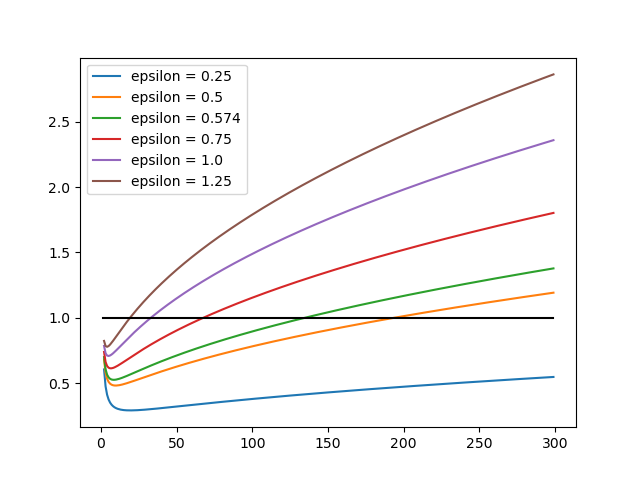
\includegraphics[scale=0.5]{figures/arithmetic.png}}
\caption{Cost comparison between the multi-block and single-block attack. The y-axis shows how much cheaper the single-block attack is. The single-block attack is more expensive when the cost reduction is less than 1. The x-axis is L$_T$.}
\label{figureCostDiff}
\end{figure}
To find the actual value of $\epsilon$ over standard values of $L_T$, we plot the ratio of multi-block to single-block attacks for $L_T$ ranging from 1 to 300 and multiple values of $\epsilon$ to get the graph in Figure \ref{figureCostDiff}\footnote{In the undercollateralization loan attack, $\epsilon$ is typically in the range 0.2 to 1. In the liquidation attack, even small values of $\epsilon$, such as 0.01 to 0.1 could be effective
in practice, given that there is a large amount of collateral that is within this range of its liquidation threshold.}. The break-even point, where both attacks have an equal cost for a 135 block TWAP oracle (which is a commonly used value in practice), is at $\epsilon = 0.574$. For higher $\epsilon$, the single-block attack is cheaper than the multi-block attack. For lower $\epsilon$, the single-block attack is more expensive. Ironically, an attacker that wants to manipulate an asset's price higher to achieve a larger profit can do so in a proportionately cheaper way. 

\subsection{Failed Assumptions}
The idea that the only way to manipulate a TWAP oracle is through the expensive multi-block attack already makes a few assumptions, like the no-arbitrage condition, an infinitely liquid external market for asset $A$ which arbitrageurs can tap into, and that arbitrageurs can always front-run the attacker's de-manipulation transaction. These assumptions have to be true to make the multi-block attack expensive for an attacker, thereby making the TWAP oracle safe to use. If the assumptions do not hold, the multi-block attack might already not be as expensive as previously thought. The single block attack, which is cheaper for larger manipulations, also makes the same assumptions. In this case, the assumptions are even less likely to hold -- thereby making the single block attack even cheaper to execute. In the following paragraphs, we give reasons why we believe these assumptions are less likely to hold: 

\textbf{No-arbitrage condition:} In the single block attack, arbitrageurs only have a single block to act, ruling out manual arbitrage, and forcing bot-based arbitrage. This general-purpose arbitrage bot needs instant access to a large amount of asset $A$. This eliminates all off-chain exchanges as reference markets since it would take at least one block to transfer funds out of the exchange.

\textbf{Infinitely liquid external market:} Eliminating off-chain exchanges also makes the assumption that arbitrageurs have access to an infinitely liquid external market less likely to hold. If arbitrageurs are unable to react within a single block, the manipulation is free.

\textbf{Transaction Ordering:} Transaction ordering within the block is even more important in the single block attack than in the multi-block attack. If the attacker can get a de-manipulation transaction included in the second block before the arbitrageur can, the attack is also free.
\bigskip

Additionally, against a multi-block attack, a DeFi protocol admin has an entire TWAP length to notice that a price is being manipulated and trigger emergency shutdown procedures if they exist. In a single-block attack, the oracle already reports the manipulated price in the very next block, and an exploit can take place immediately with no prior warning. Even if all assumptions hold, the novel result we arrive at is that for large enough $\epsilon$ and $L_T$, the cost of manipulation of a TWAP oracle only scales with the square root, not linearly with the TWAP length. If some of the assumptions do not hold, an attack may be dramatically cheaper than expected. 

In the next section, we look at a scenario where all these safety assumptions fail completely. The attacker controls a miner/proposer and can propose two blocks in a row: one with the manipulating transaction and one with the de-manipulating transaction. 

\section{Multi-Block MEV}
Miner Extractable Value (MEV) is the value that can be extracted by miners/proposers who decide which transactions go into a block and in what order. This ordering gives them the power to include their own transactions ahead of other users' transactions and thereby extract value out of the ordering process, which goes beyond their usual rewards of fees and block subsidies. Daian et al. \cite{daian2019flashboys} first explored the many ways in which transaction ordering can be used to extract more value. If an attacker could specify a transaction ordering over not just one but multiple blocks in a row, they would no longer need to compete with arbitrageurs. We call this Multi-block MEV, or MMEV. 

In the proof-of-work setting, the identity of the next successful miner is not known ahead of time. However, if a miner does selfish mining \cite{eyal2014majority,sapirshtein2016optimal,Ritz_2018} and maintains a private chain, they can publish the private chain at an opportune moment to extract more value than their share of hash power would warrant. In our case, the selfish miner has an even simpler goal -- to include their own transactions in two blocks in a row and make these two blocks get into the main blockchain. The MMEV, in this case, is the ability to cheaply manipulate a TWAP oracle, and additionally, also execute an under-collateralized loan attack or liquidation attack on a lending protocol that uses this oracle. We show that selfish mining can enable such MMEV with much lower shares of total hash power than what is traditionally expected for profitable selfish mining. Selfish mining attacks on the Uniswap V2 TWAP oracle are acknowledged in the Uniswap V2 whitepaper \cite{Adams2020UniV2} and its security audit \cite{UniswapAudit}, but has not been studied formally before.

\subsection{Manipulation Capital}
As before, the total cost of the attack consists of the manipulation capital and the attack capital. First, we assume that the attacker controls the contents of two blocks in a row and is able to execute the single block attack described earlier. This makes the manipulation capital reduce to the fees of the AMM, as there are no arbitrageurs to fight off because of selfish mining. Selfish mining itself has a cost that is independent of the attack, and we will look at that in subsequent sections.

The attacker controls two blocks. In the first block, the attacker buys $a_m$ of asset $A$, increasing the market price to $(1 + L_T \cdot \epsilon) \cdot m_p$, as required by the single block attack. This costs $b$ of asset $B$. In the first transaction in the second block, the attacker sells $a_m$ units of asset $A$, returning the market price to $m_p$, receiving $b$ units of $B$. Under normal circumstances, the transaction in the first block would be vulnerable to arbitrage. Controlling two consecutive blocks allows an attacker to be immune to arbitrage and makes the manipulation cost reduce to just the AMM fee. Note that the attacks on the lending protocol require separate attack capital that is independent of the manipulation capital we are discussing here. An MMEV attack is cheaper than a single-block attack if it is cheaper to create two blocks in a row than being vulnerable to an arbitrage that nullifies the attacker's de-manipulation transaction. The cost of selfishly mining two blocks in a row is fixed. It does not depend on $L_T$ or $\epsilon$. Assuming a constant product AMM like Uniswap V2 with $R_A \cdot R_B = K$, we can calculate the required number of tokens of asset $B$ to achieve a price for $A$ of $(1 + L_T \cdot \epsilon)\cdot m_p$ from Equation \ref{AngerisCostBound}.

Ignoring the AMM fee and assuming a TWAP length of 135 blocks (30 minutes, if we assume Ethereum as the smart contract platform), we calculate values of $b$ required for different values of $\epsilon$. Table \ref{TableCosts} shows that doubling the TWAP price of $A$ for a 30-minute TWAP (by setting $\epsilon = 1$) on a pair with \$2,000,000 of total liquidity, \$1,000,000 worth of $A$ and $B$ respectively, would require temporary capital of \$9,750,000. Increasing TWAP to $100 \cdot m_p$ (setting $\epsilon = 99$) would require temporary manipulation capital of \$113,000,000. The amount of manipulation capital required is likely a bigger limiting factor for an attacker than the cost in fees. This is an illustrative example using values for liquidity and TWAP length that could be used in practice. The manipulation capital required scales linearly with total liquidity and scales with the square root of TWAP length and $\epsilon$. Note that using a flash loan to acquire the needed funds is not an option, as this attack spans two blocks.

\begin{table}[ht]

\begin{center}
 \begin{tabular}{|c |c|} 
 \hline
 $\epsilon$ & $b$ \\ [0.5ex] 
 \hline\hline
 0.5 & 6,400,000\\ 
 \hline
 1 & 9,750,000\\ 
 \hline
 9 & 33,000,000\\ 
 \hline
 99 & 113,000,000\\  
 \hline
\end{tabular}
\end{center}
\caption{Amounts and trading fee costs for different $\epsilon$}
\label{TableCosts}
\end{table}


\subsection{Selfish Mining Cost\label{sectionSelfishMining}}
Selfish mining cost is given by the opportunity cost of not mining blocks on the main chain. We model the following miner strategy S:
The selfish miner $M$ mines on the main chain until he successfully mines a block $B_{1}$. $M$ does not publish $B_{1}$ and continues mining on top of $B_{1}$.
If $M$ finds a second block $B_{2}$, $M$ immediately publishes both $B_{1}$ and $B_{2}$. $M$'s chain is now longer than the main chain, and all honest miners will continue mining on $M$'s chain. We call this a success. If two blocks are added to the main chain without $M$ finding a block $B_{2}$, $M$ publishes $B_{1}$. This will turn $B_{1}$ into an uncle block. Then $M$ starts over and returns to mining the main chain.

\begin{figure}[h!]
\centering
\begin{tikzpicture}[auto, thick,align=center]
    %states
    \node[state] (0) {$0,0$};
    \node[state,right=of 0] (1) {$1,0$};
    \node[state,below=of 1] (2) {$1,1$};
    \node[state,right=of 1] (3) {$2,x$};
    
    %edges
    \draw [->] (0) edge[loop left] node {$1-p$} (0);
    \draw [->] (0) edge[bend left, auto=left] node {$p$} (1);
    \draw [->] (1) edge[auto=left] node {$1-p$} (2);
    \draw [->] (1) edge[bend left, auto=left] node {$p$} (3);
    \draw [->] (2) edge[bend right, auto=right] node {$p$} (3);
    \draw [->] (2) edge[bend left, auto=left] node {$1-p$} (0);
    \draw [->] (3) edge[loop right] node {$1$} (3);
    
\end{tikzpicture}
\caption{Markov chain model of strategy S}
\label{MarkovFull}
\end{figure}

Let $p$ be the share of the total hash rate that M controls. The probability of M mining any block is $p$, and the probability of all other miners mining that block is $1-p$. We assume that the propagation of newly published blocks to the network is instantaneous. Let $\mathbb{E}[S]$ be the expected number of blocks it takes to have success when following strategy S. We use the Markov chain given in Figure \ref{MarkovFull} to model strategy S. The states of the Markov chain contain pairs of $(n_1,n_2)$ with $n_1=$ number of blocks on the private chain and $n_2=$ number of blocks on the main chain. The absorbing state $(2,x)$ is the state where the selfish miner is leading with the required length 2 and will release both blocks to the main chain. As this is a finite discrete absorbing Markov chain, we can calculate the expected hitting time $\mathbb{E}[S]$ of state $(2,x)$ given the initial state is $(0,0)$ as:

\begin{align*}
    \mathbb{E}[S] = \frac{1 + 2p - p^2}{2p^2 - p^3}
\end{align*}

\noindent
\textbf{Opportunity Cost:} In the original selfish mining research on Bitcoin \cite{eyal2014majority}, the selfish miner forgoes mining rewards if the miner's private blocks do not make it to the main blockchain. In Ethereum, there is a way to reduce this opportunity cost by making these private blocks into public uncle blocks and collect uncle block rewards. It takes $\mathbb{E}[S]$ blocks for MMEV success. During this time, the miner has a $p$ chance of mining a block. This makes their uncle block opportunity $\mathbb{E}[S] \cdot p - 2$. The last two blocks cannot count as uncle blocks as the selfish miner releases them as part of the main blockchain. Uncle blocks mitigate the attack cost even more, but at the risk of exposing the fact that the attack is happening to the world at large.

\textbf{Total Cost:} In Ethereum, blocks are generated every 15 seconds, leading to 240 blocks per hour.\footnote{In practice, Ethereum has a slightly faster block generation time of ~260 blocks per hour.} The dollar cost of selfish mining is calculated based on Ethereum's total hash rate of 715 terahashes/s \cite{ethereum_hash_rate}, and the cost of renting hash power at \$60,000 for one terahash/s for 24 hours \cite{nicehash}. As we see, an attacker can rent 1.5\% hash rate for 9 hours by paying \$258,000 and expect to selfishly mine two blocks in a row. As the MMEV selfish miner has different goals than the traditional selfish miner, a much lower share of the total hash rate is enough for success. This is important because renting a higher hash rate can distort the inelastic hash rate market, and the price per hash will go up. Uncle rewards are reduced by 0.25 ETH for each generation that they are late. We remove 0.25 ETH from the average uncle block reward, putting the uncle block reward at 1.46 ETH. If we look at low values for $p$, the expected time to success (in hours) and the approximate total cost in dollars for the attack are shown in Table \ref{TableHittingTime}.
\break

\begin{table}[h!]
\begin{center}
 \begin{tabular}{|c |c| c | c | c|} 
 \hline
 $p$ & $\mathbb{E}[S]$ in hours & Cost in dollars & Uncle Rewards & Total Cost\\ [0.5ex] 
 \hline
  0.25\% & 335& \$1,499,000 & \$598,000 &\$901,000\\
  \hline
  0.50\% & 84& \$754,000 & \$298,000 &\$456,000\\
  \hline
  0.75\% & 37& \$506,000 & \$198,000 &\$308,000\\
  \hline
  1.00\% & 21& \$382,000 & \$148,000 &\$234,000\\
  \hline
  1.25\% & 13& \$307,000 & \$118,000 &\$189,000\\
  \hline
  1.50\% & 9& \$258,000 & \$98,000 &\$160,000\\
  \hline
\end{tabular}
\end{center}
\caption{Selfish Mining MMEV hash rates, costs, and rewards}
\label{TableHittingTime}
\end{table}

\subsection{MMEV in Proof of Stake}
In the proof-of-stake algorithm currently proposed for Ethereum \cite{proof_of_stake}, block proposers per epoch are known in advance. Two block proposers could collude and perform MMEV style oracle manipulation. These attacks do not go against standard consensus rules of blockchains, and hence, colluding proposers will escape slashing, or even detection.

In proof-of-stake systems that use verifiable randomness functions (Algorand, Ouroboros family), block proposers cannot be predicted in advance and MMEV attacks are not possible in the algorithms' ideal settings. However if the previous block is used to generate the seed used in the verifiable randomness function, block proposers could try a ``grinding attack'', where they try to improve their odds of proposing two blocks in a row to enable the MMEV style attack. The incentives for traditional selfish mining and ``stake grinding'' attacks are specified in terms of block rewards. However, an MMEV style attack is entirely independent of block rewards and can be orders of magnitude more profitable due to DeFi rewards. These out-sized rewards might make it worthwhile to game the verifiable randomness functions. This is an area of future research.

\section{Results}
We compare the three different TWAP manipulation attacks we have seen so far. We again use the example where we want to double the price of an asset which uses a 30-minute TWAP that uses a pair with \$2,000,000 of total liquidity reserves. The cost of the MMEV single-block attack with 1.5\% hash rate is \$160,000. Based on equation \ref{AngerisCostBound}, the cost of the single-block attack is $C_1(135 \cdot 1)$ = \$9,750,000 and the cost of the multi-block attack is $135 \cdot C_1(1)$ = \$16,200,000.
 
All attacks ignore the rather small AMM trading fee of around \$35,000. The multi-block attack (previous best known attack) cost scales linearly with the TWAP length $L_T$, whereas the single-block attack costs only scale with the square root of $L_T$. The MMEV single-block attack avoids this cost entirely as it has no arbitrageurs to worry about. The cost of selfish mining-based MMEV single block attacks only depends on the share of hash power required to pull off the attack in a reasonable time. Even with a conservative estimate of 1.5\%, it is almost two orders of magnitude cheaper than the other attacks.

\subsection{Solution 1: Median \label{sectionPotentialSolution}}
First, as seen in the commentary on Equation (\ref{AngerisCostBound}), an asset pair having high liquidity $R_A, R_B$ makes the costs of the non-MMEV attacks scale linearly with it, which mitigates the attack to some extent. In the MMEV attack, only the cost of trading fees scales with liquidity. For both the non-MMEV and MMEV variants, the amount of temporary capital required scales linearly with liquidity. Hence, illiquid assets are more likely to get attacked in the ways discussed above. 

Using a longer length for the TWAP is not ideal mitigation against the non-MMEV and MMEV attacks, as the cost and capital requirements only scale with the square root of the TWAP length in the best case. The fundamental issue that these attacks exploit is that a TWAP can be affected significantly by manipulating a single block's price. This could be solved by using a median price instead of an average. A median is largely unaffected by outlier prices in single blocks. This eliminates the single-block attack and requires the MMEV attack to take place over many blocks and not just two. Though the median makes our single block attacks harder to execute, it makes the traditional multi-block attacks easier. To manipulate a median, it is sufficient to manipulate only half the blocks it encompasses. Consequently, the multi-block attack becomes cheaper by 50\% if the median is used instead of the average.

Additionally, there are engineering issues like the calling contract having to store checkpoints to calculate the median. Storing and loading these checkpoints every time the calling contract needs an asset price can become very expensive in terms of gas costs. Optimizing these is an area of future research.

A more economic solution could be to use a median of averages with a small number of averages. One would split the block range into $n$ smaller ranges using $n+1$ checkpoints and calculate the average of each range. This would mean the majority of ranges would need to contain at least one block that is manipulated to manipulate the median. Further work would be needed to analyze the properties of such a median of averages in worst-case conditions compared to a standard median or average.

\subsection{Solution 2: Geometric Mean \label{sectionPotentialSolution2}}
Uniswap V3 stores the cumulative logarithm (to some base $b$) of the price of every pool's assets instead of the sum as in Uniswap V2. As before, we denote the length of the TWAP to be $L_T$. Say, the accumulated value of the logarithm of an asset at time $t_i$ as $$A_{t} = \sum_{i = 0}^{j = t_i}log_{b}P_i$$ This allows a consumer protocol (like a lending protocol) to use the geometric mean of the pool as
$$P_{{t_1},{t_2}} = B^{\frac{A_{t_2} - A_{t_1}}{L_T}}$$
In effect, the geometric mean of the individual prices can also be written as
$$P_{{t_1},{t_2}} = \sqrt[L_T]{\prod_{i=t_1}^{t_2} P_i}$$
To compare TWAPs with arithmetic mean and geometric mean, we assume the price of an asset to be constant (say $m_p$) over the TWAP period ($L_T$) and hence TWAPs with both arithmetic and geometric means return the same price. We now try to manipulate the TWAPs in both cases using the single block attack to reflect a price of $(1 + \epsilon)\cdot m_p$. In the case of the arithmetic mean TWAP, the price of the asset in one block has to be manipulated to $(1 + L_T \cdot \epsilon)\cdot m_p$. In the case of geometric mean TWAP, the price of the asset in one block has to be manipulated to $(1+\epsilon)^{L_T}\cdot m_p$.

\begin{figure}[h]
\centering{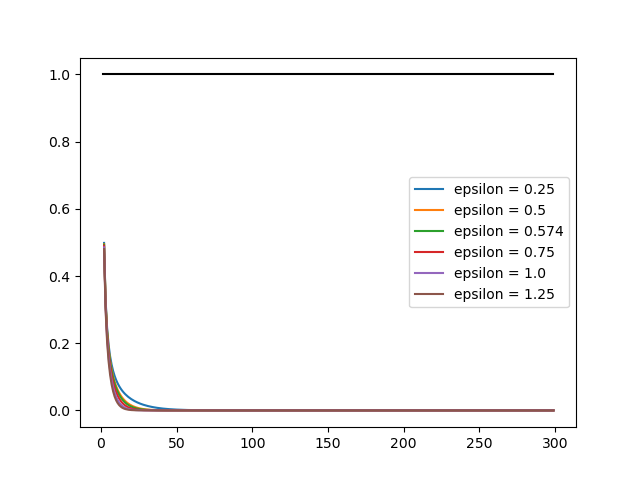
\includegraphics[scale=0.5]{figures/geometric.png}}
\caption{Cost comparison between the multi-block and single-block attack with geometric mean. The y-axis shows how much cheaper the single-block attack is. The single-block attack is more expensive when the cost reduction is less than 1. The x-axis is L$_T$.}
\label{figure_geometric}
\end{figure}

As can be seen in Figure \ref{figure_geometric}, manipulating the geometric mean by manipulating the price of an asset in a single block is more expensive than multi-block manipulation. This means that Uniswap V3 oracles are not affected by the single-block attack described in this paper, while Uniswap V2 oracles are.
However, using MMEV to avoid arbitrageurs while executing the multi-block attack could reduce its costs significantly. This would likely require controlling many blocks within the TWAP period, not just two. This makes the attack more difficult and thus more expensive. Analysing this use-case of MMEV is a topic for future research.

\section{Conclusion}
Under-collaterlaized loan attacks on the lending protocols show the need for manipulation-resistant oracles. Any protocol that relies in the same way on a TWAP oracle is vulnerable. It also turns out that the cost of manipulation for TWAP oracles is lower than expected as evidenced by the single-block attack. This attack is cheaper to execute than the previously known multi-block attack on TWAP oracles. Previously, it was assumed that TWAP oracles are safe because the multi-block attack is expensive to execute because the safeguards against the attack are assumed to work. Now we know that the single block attack is not only cheaper to execute, but the assumed safeguards do not work. One of the safeguards assumed in the multi-block attack's ``infeasibility bubble'' is that arbitrageurs can get assets from external off-chain exchanges to revert the manipulated price back to the market price. The single block attack leaves no time for arbitrageurs to do this, thereby restricting this assumption to just on-chain exchanges.

Another safeguard that is assumed in the multi-block attack's ``infeasibility bubble'' is that arbitrageurs will always arbitrage the manipulated price back to the market price. Under the MMEV setting, if an attacker can mine two blocks in a row, this no-arbitrage condition fails, and the attack gets dramatically cheaper. The area of MMEV is under-explored and should be analyzed for other exploits that are only possible when an attacker controls multiple blocks in a row. 

These attacks do not target a specific victim transaction. The goal is to manipulate an oracle that a DeFi protocol relies upon and exploit the protocol. A protocol's structural reliance on an oracle does not change much with time, and this attack is always available for the taking, based on the attacker's ability to acquire capital to pull off the attack. One solution is that TWAP oracles should use the median or the geometric mean as a manipulation-resistant statistic instead of a mean. An interesting open research question is to analyze the effect of MMEV attacks on geometric mean TWAPs or other types of metrics that also reflect an asset's true market price.

Bitcoin, with its conservative design, eschews stateful smart contracts that allow such attacks to happen. If general purpose covenants on UTXO's are enabled, we could have smart contracts on Bitcoin where such Oracle manipulation attacks are possible. It can be argued that such smart contract functionality is desirable, as it enables decentralized financial applications. We, however, believe that Bitcoin should refrain from going down the stateful smart contract route, as it enables such attacks, muddies block production incentives, and in general, takes Bitcoin away from its mission of being state-free money.

\chapterstart
\include{./chapters/conclusion}

\printbibliography

% Do not print any page numbers (or headers) after this point
\clearpage  % *after* the last page only
\pagestyle{empty}
\renewcommand\thispagestyle[1]{}  % disable chapters selecting a different pagestyle for the first page (page number in footer)  % nicer would be to only select a special first page style in \chapter when the pagestyle is not "empty"

% CV can be omitted in electronic version

\chapterstart
\chapter*{Curriculum Vitae}

% LaTeX tries to fill the page, so the layout has to be fixed with vspace...
\vspace{-5em}
\vspace{5em}
\begin{tabular}{rl}
 1979 & Born in Bangalore, India\vspace{0.5cm}\\ % normally, use three-letter month abbreviation
 1997 -- 2001 & \makecell[l]{B.E in Computer Science\\PESIT, Bangalore University, India}\vspace{0.5cm}\\
 2001 -- 2004 & \makecell[l]{Software Engineer\\ThoughtWorks India, Yahoo! India}\vspace{0.5cm}\\
 2004 -- 2006 & \makecell[l]{M.Tech. in Information Technologies\\IIT-Bombay, India}\vspace{0.5cm}\\
 2006 -- 2009 & \makecell[l]{Software Engineer, Guruji India}\vspace{0.2cm}\\ 
 2009 -- 2010 & \makecell[l]{Software Engineer, Conductor NYC}\vspace{0.2cm}\\
 2010 -- 2012 & \makecell[l]{Co-Founder, Visual Revenue NYC}\vspace{0.2cm}\\
 2012 -- 2013 & \makecell[l]{Director of Engineering, Impermium Palo Alto}\vspace{0.2cm}\\
 2013 -- 2018 & \makecell[l]{Software Engineer, Google Z{\"u}rich}\vspace{0.5cm}\\
 2018 -- 2023 & \makecell[l]{Ph.D. Student (Doctor of Sciences)\\Distributed Computing Group, ETH Z{\"u}rich}\vspace{0.5cm}
\end{tabular}


\end{document}